% TeX TXS-program:compile = txs:///pdflatex/[-shell-escape]
\documentclass[a4paper,12pt,oneside]{scrartcl}
\pdfminorversion=7
\usepackage[a4paper,
textheight = 700pt,
marginparsep=0.5cm,
textwidth=7in,
marginparwidth=1cm]{geometry}

\usepackage[mathjax,                     % Math via MathJax in HTML
	HomeHTMLFilename=index,      % homepage filename
	HTMLFilename={node-},         % per-page filename prefix
	ImagesDirectory=main-images,
	OSWindows,
]{lwarp}
\boolfalse{FileSectionNames}

\HTMLTitle{Plotting}
\HTMLAuthor{Dima Bykhovsky}
\HTMLDescription{Plotting for engineers: visual perception, color and colormaps, choosing the encoding, axes, fonts, transparency, and figures inside a document.}
\HTMLLanguage{en-US}
\CSSFilename{lwarp_academic.css}
% Section name first, document title appended: search engines truncate <title> at
% roughly 65 characters, and the repeated title is the part worth losing.
\HTMLTitleAfterSection
\setcounter{FileDepth}{1}      % split HTML at \section
\setcounter{SideTOCDepth}{2}   % side TOC depth
\booltrue{CombineHigherDepths}

\begin{warpMathJax}
	\CustomizeMathJax{
		\newcommand{\abs}[1]{\lvert#1\rvert}
	}
	\CustomizeMathJax{
		\DeclareMathOperator{\sign}{sign}
	}
\end{warpMathJax}

\usepackage{amsmath,amsthm,amssymb,mathrsfs,amsfonts,bm, bbm}
\usepackage{physics}
\usepackage{cancel}

%\usepackage{mathtools}
\let\Re\undefined
\let\Im\undefined
\DeclareMathOperator{\Re}{\mathscr{R}}
\DeclareMathOperator{\Im}{\mathscr{I}}
%https://tex.stackexchange.com/questions/1372/typeset-reaib

\newtheorem{theorem}{Theorem}


% https://tex.stackexchange.com/questions/54846/under-up-arrow-text
\newcommand*{\underuparrow}[1]{{\underset{\uparrow}{#1}}} \CustomizeMathJax{\newcommand{\underuparrow}[1]{{\underset{\uparrow}{#1}}}}


%%% --- Configurations ---
%https://tex.stackexchange.com/questions/36039/automatic-size-adjustment-for-nested-parentheses
\delimitershortfall=-1pt

%https://tex.stackexchange.com/questions/51682/is-it-possible-to-pagebreak-aligned-equations
\allowdisplaybreaks

%%% --- Definitions ---
\DeclareMathOperator*{\argmax}{argmax}
\CustomizeMathJax{\DeclareMathOperator*{\argmax}{argmax}}
\DeclareMathOperator*{\argmin}{arg\,min}
\CustomizeMathJax{\DeclareMathOperator*{\argmin}{arg\,min}}
%\newcommand{\argmax}[1]{ \arg\,\max\limits_{#1}}
%\newcommand{\argmin}[1]{ \arg\,\min\limits_{#1}}

\newcommand{\floor}[1]{\lfloor #1 \rfloor}

\CustomizeMathJax{%
	\def\E[#1]{\mathbb{E}\!\left[ #1 \right]}%
}


\NewDocumentCommand\E{D(){}o}{%
	{\mathbb{E}}^{#1}\!\left[{#2}\right]
}
%----
\CustomizeMathJax{%
	\def\Var[#1]{\operatorname{Var}\!\left[ #1 \right]}%
}

\NewDocumentCommand\Var{D(){}o}{%
	{\mathrm{Var}}^{#1}\!\left[{#2}\right]
}
%----
\CustomizeMathJax{%
	\def\Cov[#1]{\operatorname{Cov}\!\left[ #1 \right]}%
}

\NewDocumentCommand\Cov{o}{%
	\mathrm{Cov}\!\left[{#1}\right] %
}
\DeclareMathOperator{\sign}{sign}
\DeclareMathOperator{\diag}{diag}
%\overset{\displaystyle\mathscr F}{\Longleftrightarrow}
\newcommand{\DTFTH}{ H \brk1{e^{j\omega}}}
\newcommand{\DTFTX}{ X\brk1{e^{j\omega}}}
\newcommand{\DFTtr}[1]{\mathrm{DFT}\left\{#1\right\}}
\newcommand{\DTFTtr}[1]{\mathrm{DTFT}\left\{#1\right\}}
\newcommand{\DTFTtrI}[1]{\mathrm{DTFT^{-1}}\left\{#1\right\}}
\newcommand{\Ftr}[1]{ \mathcal{F}\left\{#1\right\}}
\newcommand{\FtrI}[1]{ \mathcal{F}^{-1}\left\{#1\right\}}

\newcommand{\SSE}{\mathrm{SSE}}
\newcommand{\SST}{\mathrm{SST}}
\newcommand{\SSR}{\mathrm{SSR}}
\newcommand{\MSE}{\mathrm{MSE}}
\newcommand{\RMSE}{\mathrm{RMSE}}

\newcommand{\Zover}{\overset{\mathscr Z}{\Longleftrightarrow}}
\renewcommand{\real}{\mathbb{R}}
\newcommand{\ba}{\mathbf{a}}
\newcommand{\bb}{\mathbf{b}}
\newcommand{\bc}{\mathbf{c}}
\newcommand{\bd}{\mathbf{d}}
\newcommand{\be}{\mathbf{e}}
\newcommand{\bf}{\mathbf{f}}
\newcommand{\bg}{\mathbf{g}}
\newcommand{\bh}{\mathbf{h}}
\newcommand{\bi}{\mathbf{i}}
\newcommand{\bn}{\mathbf{n}}
\newcommand{\bo}{\mathbf{o}}
\newcommand{\bp}{\mathbf{p}}
\newcommand{\bq}{\mathbf{q}}
\newcommand{\br}{\mathbf{r}}
\newcommand{\bs}{\mathbf{s}}
\newcommand{\bt}{\mathbf{t}}
\newcommand{\bu}{\mathbf{u}}
\newcommand{\bv}{\mathbf{v}}
\newcommand{\bw}{\mathbf{w}}
\newcommand{\bx}{\mathbf{x}}
\newcommand{\bxx}{\mathbf{xx}}
\newcommand{\bxy}{\mathbf{xy}}
\newcommand{\by}{\mathbf{y}}
\newcommand{\byx}{\mathbf{yx}}
\newcommand{\byy}{\mathbf{yy}}
\newcommand{\bz}{\mathbf{z}}

\newcommand{\bA}{\mathbf{A}}
\newcommand{\bB}{\mathbf{B}}
\newcommand{\bC}{\mathbf{C}}
\newcommand{\bD}{\mathbf{D}}
\newcommand{\bH}{\mathbf{H}}
\newcommand{\bI}{\mathbf{I}}
\newcommand{\bK}{\mathbf{K}}
\newcommand{\bM}{\mathbf{M}}
\newcommand{\bP}{\mathbf{P}}
\newcommand{\bQ}{\mathbf{Q}}
\newcommand{\bR}{\mathbf{R}}
\newcommand{\bS}{\mathbf{S}}
\newcommand{\bU}{\mathbf{U}}
\newcommand{\bW}{\mathbf{W}}
\newcommand{\bX}{\mathbf{X}}
\newcommand{\bY}{\mathbf{Y}}
\newcommand{\bZ}{\mathbf{Z}}

\newcommand{\balpha}{\bm{\alpha}}
\newcommand{\bth}{{\bm{\theta}}}
\newcommand{\bepsilon}{{\bm{\epsilon}}}
\newcommand{\bmu}{{\bm{\mu}}}
\newcommand{\bgamma}{{\bm{\gamma}}}
\newcommand{\bphi}{\bm{\phi}}
\newcommand{\bOne}{\mathbf{1}}
\newcommand{\bZero}{\mathbf{0}}
\newcommand{\indFunc}{\mathbbm{1}}
\newcommand{\btx}{\tilde{\bx}}
\newcommand{\loss}{\mathcal{L}}
\newcommand{\score}{\mathcal{S}}

\CustomizeMathJax{\newcommand{\floor}[1]{\lfloor #1 \rfloor}}
\CustomizeMathJax{\newcommand{\DTFTH}{ H \brk1{e^{j\omega}}}}
\CustomizeMathJax{\newcommand{\DTFTX}{ X\brk1{e^{j\omega}}}}
\CustomizeMathJax{\newcommand{\DFTtr}[1]{\mathrm{DFT}\left\{#1\right\}}}
\CustomizeMathJax{\newcommand{\DTFTtr}[1]{\mathrm{DTFT}\left\{#1\right\}}}
\CustomizeMathJax{\newcommand{\DTFTtrI}[1]{\mathrm{DTFT^{-1}}\left\{#1\right\}}}
\CustomizeMathJax{\newcommand{\Ftr}[1]{ \mathcal{F}\left\{#1\right\}}}
\CustomizeMathJax{\newcommand{\FtrI}[1]{ \mathcal{F}^{-1}\left\{#1\right\}}}

\CustomizeMathJax{\newcommand{\Zover}{\overset{\mathscr Z}{\Longleftrightarrow}}}
\CustomizeMathJax{\renewcommand{\real}{\mathbb{R}}}
\CustomizeMathJax{\newcommand{\ba}{\mathbf{a}}}
\CustomizeMathJax{\newcommand{\bb}{\mathbf{b}}}
\CustomizeMathJax{\newcommand{\bc}{\mathbf{c}}}
\CustomizeMathJax{\newcommand{\bd}{\mathbf{d}}}
\CustomizeMathJax{\newcommand{\be}{\mathbf{e}}}
\CustomizeMathJax{\newcommand{\bf}{\mathbf{f}}}
\CustomizeMathJax{\newcommand{\bg}{\mathbf{g}}}
\CustomizeMathJax{\newcommand{\bh}{\mathbf{h}}}
\CustomizeMathJax{\newcommand{\bi}{\mathbf{i}}}
\CustomizeMathJax{\newcommand{\bn}{\mathbf{n}}}
\CustomizeMathJax{\newcommand{\bo}{\mathbf{o}}}
\CustomizeMathJax{\newcommand{\bp}{\mathbf{p}}}
\CustomizeMathJax{\newcommand{\bq}{\mathbf{q}}}
\CustomizeMathJax{\newcommand{\br}{\mathbf{r}}}
\CustomizeMathJax{\newcommand{\bs}{\mathbf{s}}}
\CustomizeMathJax{\newcommand{\bt}{\mathbf{t}}}
\CustomizeMathJax{\newcommand{\bu}{\mathbf{u}}}
\CustomizeMathJax{\newcommand{\bv}{\mathbf{v}}}
\CustomizeMathJax{\newcommand{\bw}{\mathbf{w}}}
\CustomizeMathJax{\newcommand{\bx}{\mathbf{x}}}
\CustomizeMathJax{\newcommand{\bxx}{\mathbf{xx}}}
\CustomizeMathJax{\newcommand{\bxy}{\mathbf{xy}}}
\CustomizeMathJax{\newcommand{\by}{\mathbf{y}}}
\CustomizeMathJax{\newcommand{\byx}{\mathbf{yx}}}
\CustomizeMathJax{\newcommand{\byy}{\mathbf{yy}}}
\CustomizeMathJax{\newcommand{\bz}{\mathbf{z}}}

\CustomizeMathJax{\newcommand{\bA}{\mathbf{A}}}
\CustomizeMathJax{\newcommand{\bB}{\mathbf{B}}}
\CustomizeMathJax{\newcommand{\bC}{\mathbf{C}}}
\CustomizeMathJax{\newcommand{\bD}{\mathbf{D}}}
\CustomizeMathJax{\newcommand{\bH}{\mathbf{H}}}
\CustomizeMathJax{\newcommand{\bI}{\mathbf{I}}}
\CustomizeMathJax{\newcommand{\bK}{\mathbf{K}}}
\CustomizeMathJax{\newcommand{\bM}{\mathbf{M}}}
\CustomizeMathJax{\newcommand{\bP}{\mathbf{P}}}
\CustomizeMathJax{\newcommand{\bQ}{\mathbf{Q}}}
\CustomizeMathJax{\newcommand{\bR}{\mathbf{R}}}
\CustomizeMathJax{\newcommand{\bS}{\mathbf{S}}}
\CustomizeMathJax{\newcommand{\bU}{\mathbf{U}}}
\CustomizeMathJax{\newcommand{\bW}{\mathbf{W}}}
\CustomizeMathJax{\newcommand{\bX}{\mathbf{X}}}
\CustomizeMathJax{\newcommand{\bY}{\mathbf{Y}}}
\CustomizeMathJax{\newcommand{\bZ}{\mathbf{Z}}}

\CustomizeMathJax{\newcommand{\balpha}{\bm{\alpha}}}
\CustomizeMathJax{\newcommand{\bth}{{\bm{\theta}}}}
\CustomizeMathJax{\newcommand{\bepsilon}{{\bm{\epsilon}}}}
\CustomizeMathJax{\newcommand{\bmu}{{\bm{\mu}}}}
\CustomizeMathJax{\newcommand{\bgamma}{{\bm{\gamma}}}}
\CustomizeMathJax{\newcommand{\bphi}{\bm{\phi}}}
\CustomizeMathJax{\newcommand{\bOne}{\mathbf{1}}}
\CustomizeMathJax{\newcommand{\bZero}{\mathbf{0}}}
\CustomizeMathJax{\newcommand{\indFunc}{\mathbb{1}}}
\CustomizeMathJax{\newcommand{\btx}{\tilde{\bx}}}
\CustomizeMathJax{\newcommand{\loss}{\mathcal{L}}}
\CustomizeMathJax{\newcommand{\score}{\mathcal{S}}}

\CustomizeMathJax{\newcommand{\SSE}{\mathrm{SSE}}}
\CustomizeMathJax{\newcommand{\SST}{\mathrm{SST}}}
\CustomizeMathJax{\newcommand{\SSR}{\mathrm{SSR}}}
\CustomizeMathJax{\newcommand{\MSE}{\mathrm{MSE}}}
\CustomizeMathJax{\newcommand{\RMSE}{\mathrm{RMSE}}}
% lwarp reads the equation-number prefix from amsmath's \numberwithin bookkeeping;
% without it MathJax tags every displayed equation with a bare "n".
\numberwithin{equation}{section}
\counterwithin{figure}{section}
\counterwithin{table}{section}
\usepackage{xurl}
\usepackage{placeins}
\usepackage{parskip}
\usepackage{enumitem}
\setlist[itemize]{noitemsep, nosep}
\setlength\parindent{0pt}


\usepackage{array}
\newcolumntype{L}[1]{>{\raggedright\let\newline\\\arraybackslash\hspace{0pt}}m{#1}}
\newcolumntype{C}[1]{>{\centering\let\newline\\\arraybackslash\hspace{0pt}}m{#1}}
\newcolumntype{R}[1]{>{\raggedleft\let\newline\\\arraybackslash\hspace{0pt}}m{#1}}
%https://tex.stackexchange.com/questions/12703/how-to-create-fixed-width-table-columns-with-text-raggedright-centered-raggedlef
% lwarp parses tabular preambles itself and does not know that L/C/R take an
% argument, so it miscounts columns and misplaces the | rules in the HTML output.
% Register the HTML equivalents. Widths are irrelevant in HTML (cells wrap on
% their own); only the type letter matters, as it picks the tdl/tdc/tdr class.
% Use l/c/r rather than m{#1}: paragraph-mode columns make lwarp emit a <p>
% inside each cell, which is not wanted for these one-paragraph cells.
\HTMLnewcolumntype{L}[1]{l}
\HTMLnewcolumntype{C}[1]{c}
\HTMLnewcolumntype{R}[1]{r}

\usepackage{url}

%https://tex.stackexchange.com/questions/120777/more-than-two-figures-on-one-page-with-text-in-between-problem-with-float
\renewcommand\textfraction{.1}
\setcounter{totalnumber}{5}

%	HEADERS AND FOOTERS
\usepackage{fancyhdr} % Required for header and footer configuration
\pagestyle{fancy} % Enable the custom headers and footers
\renewcommand{\sectionmark}[1]{\markright{\normalsize\thesection\hspace{5pt}#1}{}} % Styling for the current section in the header
\fancyhf{} % Clear default headers and footers
\fancyhead[LE,RO]{\sffamily\normalsize\thepage} % Styling for the page number in the header
%\fancyhead[LO]{\rightmark} % Print the nearest section name on the left side of odd pages
%\fancyhead[RE]{\leftmark} % Print the current chapter name on the right side of even pages
%\fancyfoot[C]{\thepage} % Uncomment to include a footer
%https://tex.stackexchange.com/questions/327285/what-does-this-warning-mean-fancyhdr-and-headheight
%\setlength{\headheight}{15pt}

\renewcommand{\headrulewidth}{0.5pt} % Thickness of the rule under the header
\fancypagestyle{plain}{% Style for when a plain pagestyle is specified
	\fancyhead{}\renewcommand{\headrulewidth}{0pt}%
}
% Removes the header from odd empty pages at the end of chapters
\makeatletter
\renewcommand{\cleardoublepage}{
	\clearpage\ifodd\c@page\else
	\hbox{}
	\vspace*{\fill}
	\thispagestyle{empty}
	\newpage
	\fi}

% compress the text up at the bottom of the page
\raggedbottom 



\usepackage{booktabs,multirow,array,float}
\usepackage{tabularx}

\usepackage{tcolorbox}
\tcbuselibrary{skins,xparse,breakable}
\usepackage{colortbl}
\usepackage{siunitx}
% lwarp's siunitx emulation defines the unit abbreviations as global MathJax macros,
% among them \pm = picometre, which turns every \pm on every HTML page into "pm".
% Restore the plus-minus sign (binary operator, as in TeX).
\CustomizeMathJax{\renewcommand{\pm}{\mathbin{\unicode{x00B1}}}}
% Decimal-aligned number columns. Both are the siunitx S column in the PDF; lwarp's
% HTML S column is centered, so the HTML twins pick the alignment that lines the
% decimal points up there (the CSS sets tabular figures for table cells). Redefining
% S itself for HTML fails: lwarp-siunitx defines it only at \begin{document}.
%   N{2.1}: a fixed number of decimals, so right alignment is decimal alignment.
%   P: one integer digit and varying decimals (5, 1.3, 0.0001), so left alignment is.
\newcolumntype{N}[1]{S[table-format=#1]}
\HTMLnewcolumntype{N}[1]{r}
\newcolumntype{P}{S[table-format=1.4]}
\HTMLnewcolumntype{P}{l}
\usepackage{subcaption}
\captionsetup[subfigure]{position=bottom,justification=raggedright,singlelinecheck=false}
\usepackage{graphicx}
\graphicspath{{figs/}}

\newtheoremstyle{goal}%
{}{}%
{}{}%
{}%
{}%
{ }%
{\textbf{\color{blue!50}#1}}
\theoremstyle{goal}
\newtheorem{goal}{Goal:}

\renewcommand\qedsymbol{}
\setlength{\topsep}{0pt}

% Box environments: red = hard errors, yellow = caveats, blue = clarifications.
\NewTColorBox{box_red}{ !O{} }{
	breakable,
	enhanced,
	colframe=red!70!black,
	colbacktitle=white,
	coltitle=red!70!black,
	fonttitle=\bfseries,
	IfValueT={#1}{attach boxed title to top left={xshift=1cm,yshift=-2mm}, title={#1}, boxed title style={colback=white,colframe=red!70!black}}
}

\NewTColorBox{box_yellow}{ !O{} }{
	breakable,
	enhanced,
	colframe=orange!75!black,
	colbacktitle=white,
	coltitle=orange!80!black,
	fonttitle=\bfseries,
	IfValueT={#1}{attach boxed title to top left={xshift=1cm,yshift=-2mm}, title={#1}, boxed title style={colback=white,colframe=orange!75!black}}
}

\NewTColorBox{box_blue}{ !O{} }{
	breakable,
	enhanced,
	colframe=blue!40!white,
	colbacktitle=white,
	coltitle=blue!40!black,
	fonttitle=\bfseries,
	IfValueT={#1}{attach boxed title to top left={xshift=1cm,yshift=-2mm}, title={#1}, boxed title style={colback=white,colframe=blue!40!white}}
}

% lwarp's tcolorbox emulation only renders a title bar from a plain title= key;
% the "attach boxed title" style above produces no HTML title. Redefine for HTML
% with a plain title (colored bar, white text) so titles appear in HTML output.
\begin{warpHTML}
\RenewTColorBox{box_red}{ !O{} }{
	colframe=red!70!black,
	coltitle=white,
	fonttitle=\bfseries,
	IfValueT={#1}{title={#1}}
}
\RenewTColorBox{box_yellow}{ !O{} }{
	colframe=orange!75!black,
	coltitle=white,
	fonttitle=\bfseries,
	IfValueT={#1}{title={#1}}
}
\RenewTColorBox{box_blue}{ !O{} }{
	colframe=blue!40!white,
	coltitle=white,
	fonttitle=\bfseries,
	IfValueT={#1}{title={#1}}
}
\end{warpHTML}

\usepackage[colorlinks,bookmarksopen,bookmarksnumbered,citecolor=red,urlcolor=red]{hyperref}
\PassOptionsToPackage{
	type={CC},
	modifier={by-nc-sa},
	version={4.0}
}{doclicense}
\usepackage{doclicense}

\begin{document}
\title{Plotting}
\author{Dima Bykhovsky}
\maketitle

\noindent This is an on-going project that is frequently updated. The author assumes no responsibility for errors or omissions.

\doclicenseLongText

\setcounter{tocdepth}{1}
\tableofcontents
\begin{warpHTML}
Link to \href{plottingc.pdf}{PDF version} of this document.
\end{warpHTML}

This document collects how figures should be prepared: which visual channels a reader can actually decode, which ones only look informative, and which library defaults quietly damage the result. The rules are few, they are supported by measurement rather than taste, and at least some of them are violated by the first plot any tool produces.

\begin{goal}
Present rules and guidelines for an effective visual presentation of engineering information.
\end{goal}
\begin{quote}
"There are three kinds of lies: lies, damned lies, and statistics"

Various Attributions  
\end{quote}
\section{Preface}


\section{A Chart That Cost a Space Vehicle}\label{sec-app-plot-challenger}
\subsection{The Story}
On the evening of 27 January 1986, engineers at Morton Thiokol recommended against launching the Space Shuttle \emph{Challenger} the next morning. Their concern was the temperature: the rubber O-rings sealing the joints of the solid rocket boosters stiffen in the cold, and the forecast overnight low was far below anything the program had flown in. They had the flight history to support the concern. 
But they did not have was a chart that clearly showed it.

Fig.~\ref{fig-plot-thiokol} is one of the charts they presented. It carries the whole damage record: twenty-four booster pairs, the O-ring temperature (${}^\circ$F)of each, and every erosion and blow-by incident that had been found on recovery.

\begin{figure}[ht]
	\centering
	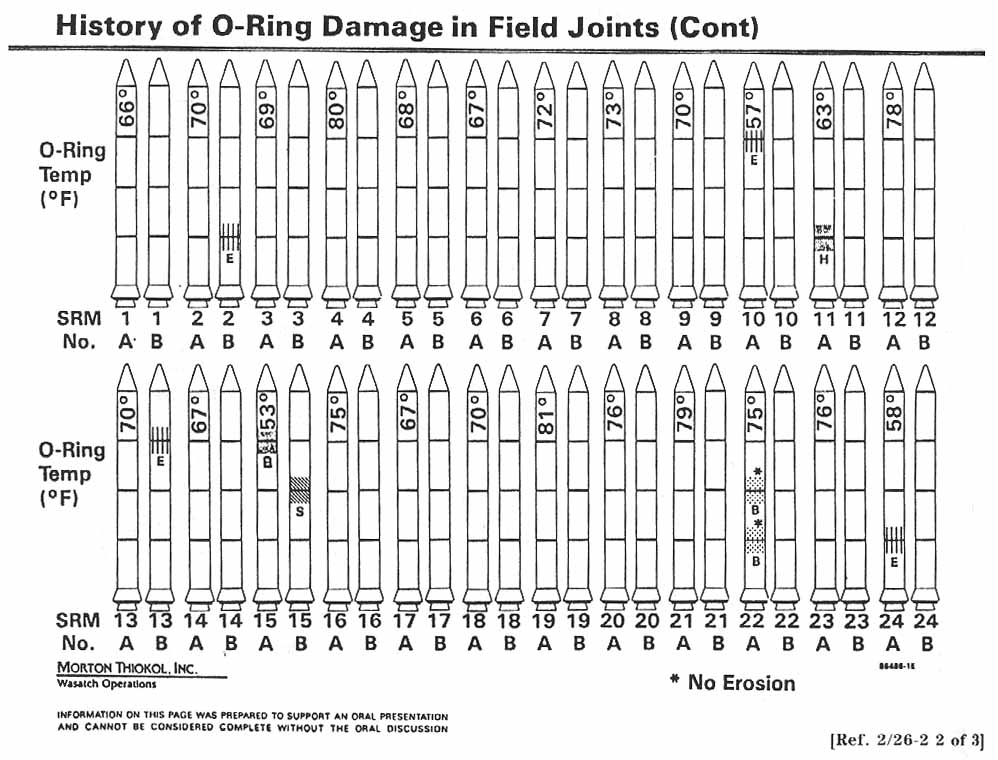
\includegraphics[width=0.92\textwidth]{challenger_thiokol}
	\caption{``History of O-Ring Damage in Field Joints'', presented by Morton Thiokol on 27 January 1986. Every number needed for the decision is on this page. Temperature appears as rotated text inside each rocket, damage as hatch marks and single letters, and the flights run in launch order. Reproduced from the \emph{Report of the Presidential Commission on the Space Shuttle Challenger Accident}, Vol.~5, p.~896, a work of the U.S. Government in the public domain, \url{https://www.nasa.gov/history/rogersrep/v5p896.htm}.}
	\label{fig-plot-thiokol}
\end{figure}

Read it against the rest of this document and it fails on nearly every count at once:
\begin{itemize}
	\item The forty-eight rocket outlines are decoration: they encode nothing, and they consume most of the page (Sec.~\ref{sec-app-plot-dataink}). 
	\item Temperature, the quantity the entire argument turns on, is printed as rotated text inside each drawing rather than given a position on an axis, which is the one channel a reader decodes accurately (Sec.~\ref{sec-app-plot-encoding}). 
	\item Damage is encoded as unexplained hatch patterns and the letters \texttt{E}, \texttt{B} and \texttt{S}. 
	\item The flights are ordered by booster number, so the coldest launch on record sits in the middle of the second row with nothing to distinguish it. The relation between temperature and damage is present in this chart and cannot be read from it.
\end{itemize}


\subsection{The same data on axes}

Fig.~\ref{fig-plot-challenger} plots the identical record. The horizontal axis is temperature, the vertical axis is the number of O-rings damaged on that launch, and nothing else is on the page.

\begin{figure}[ht]
	\centering
	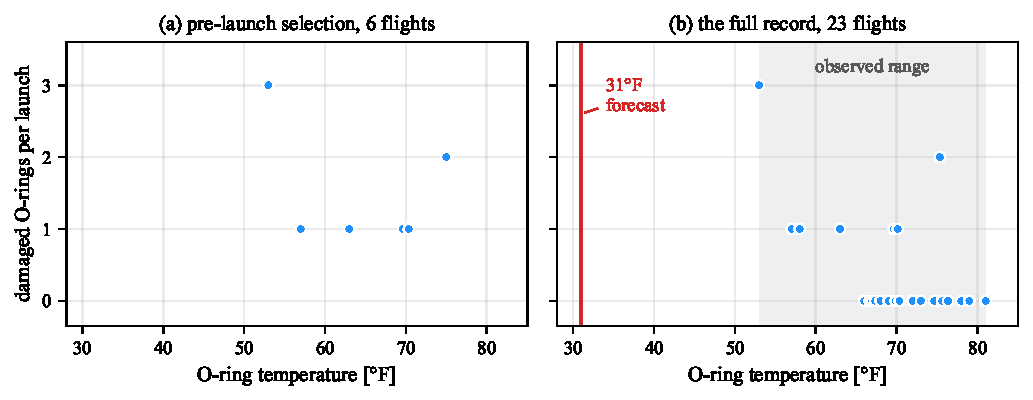
\includegraphics{plot_challenger}
	\caption{The O-ring record of the $23$ flights preceding \emph{Challenger}, plotted twice.\\
		(a) The six damage flights that the pre-launch discussion centered on. Damage occurs from $53$ to $75\,^{\circ}$F with no visible trend, which is the reading that was available on the night.\\
		(b) The same record with the undamaged flights restored: all four launches at or below $63\,^{\circ}$F were damaged, while only $3$ of the $19$ warmer ones were. The vertical line marks the $31\,^{\circ}$F forecast for the launch morning and the shaded band the range ever flown. Tied points are spread horizontally by up to $0.35\,^{\circ}$F so that the four flights at $70\,^{\circ}$F can be counted. Data: \texttt{orings} from the R package \texttt{DAAG}, after the Presidential Commission report, Vol.~1, pp.~129--131. }
	\label{fig-plot-challenger}
\end{figure}

The two panels differ only in which flights they contain. Panel~(a) holds the flights that showed damage, which is roughly the selection the argument was built from: six points between $53$ and $75\,^{\circ}$F, no pattern, and therefore no case. Panel~(b) restores the seventeen launches that came back clean. Those seventeen are not absence of evidence; each one is a launch at a known temperature that produced no damage, and they are what turns a scatter of incidents into a relation. Every launch at or below $63\,^{\circ}$F was damaged. Only three of the nineteen above it were.

The vertical line is the forecast for the following morning, $31\,^{\circ}$F, which is $22\,^{\circ}$F colder than the coldest launch ever attempted.

\begin{box_blue}[What the case actually shows]
	The engineers were right, they had the data, and they presented it. The failure was in the encoding. A chart that places the causal variable on an axis takes about a minute to make from the same numbers, and it makes the argument by itself. That is the claim this document defends: plotting is a technical skill with a right and a wrong answer, not a matter of presentation polish applied after the analysis is finished.
\end{box_blue}

\section{Why Plot at All}\label{sec-app-plot-why}
\begin{goal}
Why plot?
\end{goal}

Fig.~\ref{fig-plot-anscombe} shows four datasets constructed by Anscombe in 1973. All four have:
\begin{itemize}
	\item  mean $9.00$ in $x$
	\item mean  $7.50$ in $y$, 
	\item variance $10.00$ and $3.75$ (with the $1/n$ normalization), 
	\item correlation $0.816$, and 
	\item least-squares fit $\hat{y} = 3.00 + 0.50x$.
\end{itemize} 
\begin{box_red}
Every standard summary of a bivariate relation (means, variances, correlation, and the regression line) is identical across the four panels, to two decimals.
\end{box_red}

\begin{figure}[ht]
	\centering
	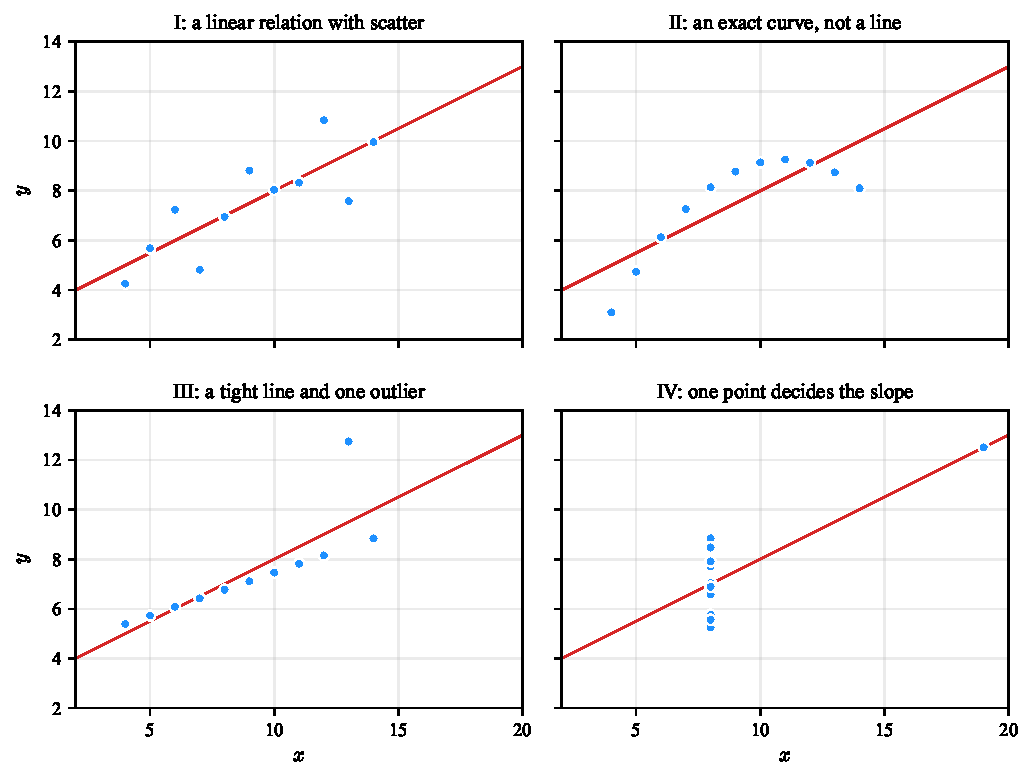
\includegraphics{plot_anscombe}
	\caption{Anscombe's quartet.}
	\label{fig-plot-anscombe}
\end{figure}

This is the reason exploratory analysis should lead with plots. The five-number summary behind a boxplot is a compression, and the violin plot exists precisely because a boxplot cannot show that a distribution has two modes. The same argument runs one level up: a statistic is a compression of a plot, and a plot is a compression of the data. Each step discards structure, and the discarded structure is where the modeling errors hide.
\FloatBarrier
\section{What the Eye Does for Free}\label{sec-app-plot-perception}

Sight carries more information per second than the other senses combined, but it does not deliver that bandwidth uniformly. Table~\ref{tab-plot-senses} puts numbers on the first claim: the eyes alone move about $10^{7}$~bit/s, and the five channels together deliver roughly $11$~million~bit/s to the brain. Conscious processing keeps up with only about $50$~bit/s, so almost everything is discarded before it reaches awareness. A chart is a device for choosing what survives that reduction, and it is effective in proportion to how much of the reader's throughput it spends on the data rather than on decoding the chart.

\begin{table}[ht]
	\centering
	\caption{Information transmission rates of the five senses. The eyes carry two orders of magnitude more than the ears, and the five channels together deliver about $11$~million~bit/s, while conscious processing handles only about $50$~bit/s. That gap of more than five orders of magnitude is the compression every figure in this document is trying to help the reader perform. After the \emph{Encyclop\ae dia Britannica} entry on information theory.}
	\label{tab-plot-senses}
	\begin{tabular}{L{5cm}|R{4cm}}
		\hline
		\textit{Sensory system} & \textit{Bits per second} \\
		\hline
		Eyes  & 10,000,000 \\
		Skin  & 1,000,000 \\
		Ears  & 100,000 \\
		Smell & 100,000 \\
		Taste & 1,000 \\
		\hline
	\end{tabular}
\end{table}

Visual processing runs in two stages:
\begin{enumerate}
	\item The first stage is \emph{pre-attentive}: a small set of features is extracted from the entire visual field in parallel, in roughly the $200$~ms between one eye movement and the next, without conscious effort and without regard to how many objects are present. The list is short and has been established experimentally: length, width, size, curvature, number, line ends, intersection, closure, color, how light or dark a mark is, flicker, direction of motion, and a few depth cues. \newline
The second stage is \textit{serial}. It identifies objects and their arrangement, it consults memory, and its cost grows with the number of items to be examined.

\end{enumerate}
Fig.~\ref{fig-plot-preattentive-features} shows each of these channels in isolation: in every small grid one mark differs from the rest along a single feature, and the eye lands on it without a search.

\begin{figure}[ht]
	\centering
	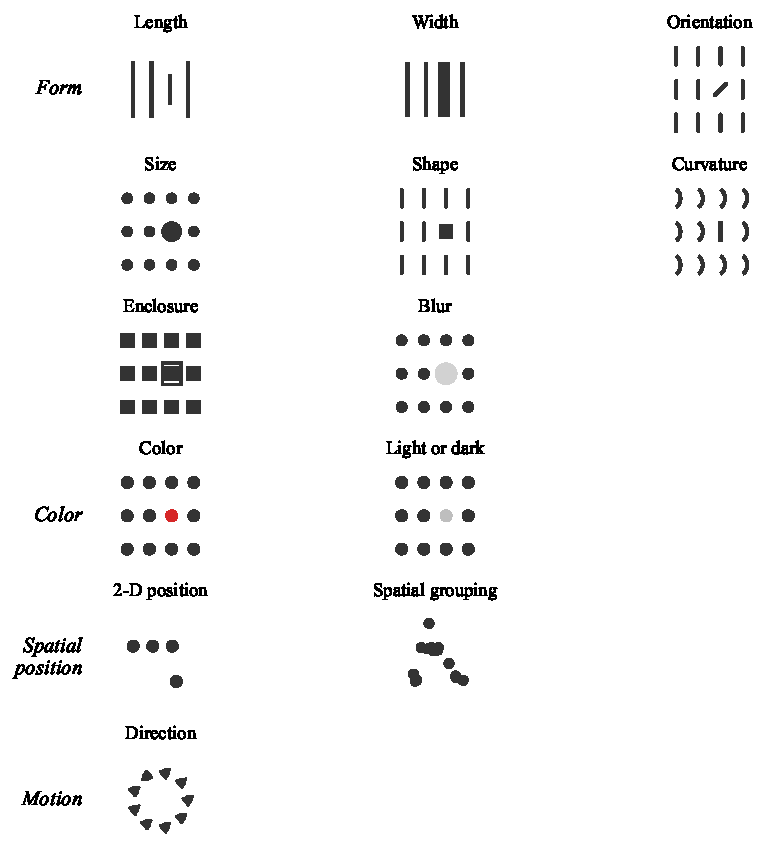
\includegraphics{plot_preattentive_features}
	\caption{The pre-attentive attributes, one small grid each, grouped as \emph{Form}, \emph{Color}, \emph{Spatial position} and \emph{Motion}. Every grid hides a single odd element, and it is found without a search. Flicker and direction of motion are pre-attentive on the same footing but cannot be shown on a static page, so \emph{Direction} only hints a heading through the arrows. After Few, \emph{Show Me the Numbers} (2012), via the DLI human-perception slides.}
	\label{fig-plot-preattentive-features}
\end{figure}

The three demonstrations of Fig.~\ref{fig-plot-preattentive} show what the difference between the two stages feels like.

\begin{figure}[ht]
	\centering
	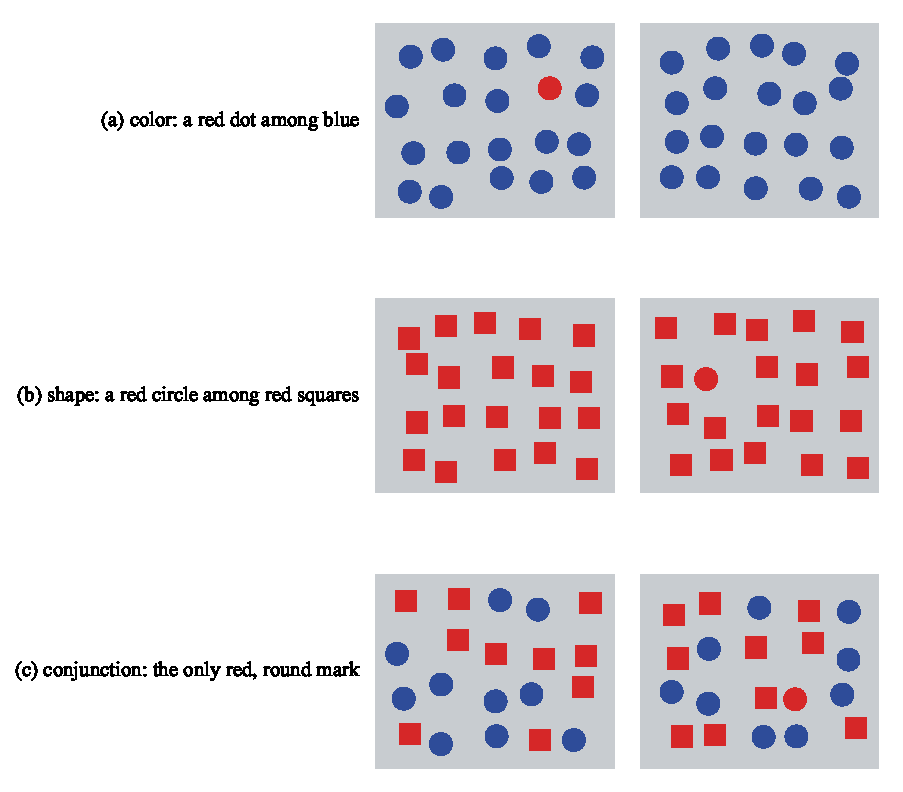
\includegraphics{plot_preattentive}
	\caption{Three single-feature searches, each posed the way the source poses it: which side holds the odd mark? (a) A red dot among blue and (b) a red circle among red squares are answered before the eye has moved, however many marks are present, because color and shape are each pre-attentive. (c) The target is the only mark that is both red \emph{and} round, among blue circles and red squares; that conjunction is not pre-attentive, so the side can be found only by checking marks one at a time.}
	\label{fig-plot-preattentive}
\end{figure}

The practical consequence is the third row. A reader can be asked to find the red mark, or the round mark, and will find it instantly however many distractors there are. A reader asked to find the mark that is red \textit{and} round has to inspect the marks one at a time, and the time taken grows with their number. \begin{box_blue}
Encoding one variable in color and a second in marker shape, and then asking the reader to locate a particular combination. Two channels are fine for two independent readings, and they fail for a conjunction.
\end{box_blue}

\FloatBarrier
\subsection{Two ways a graph is read}\label{sec-app-plot-lookup}

A reader arrives at a figure with one of two questions, and the two are served by different halves of the machinery above. 
\begin{itemize}
	\item \emph{Pattern perception} asks what the shape is: which values are large, where the group boundaries fall, whether the decay is smooth. It rides the parallel stage, so it is free and it scales, and twenty marks are taken in as fast as five.
	\item  \emph{Table look-up} asks for one named item and its value.\footnote{The two operations are Cleveland's, and the experiments that measured the encodings behind them are Cleveland and McGill, \href{https://doi.org/10.1080/01621459.1984.10478080}{``Graphical Perception: Theory, Experimentation, and Application to the Development of Graphical Methods''}, \emph{J.\ American Statistical Association}, vol.~79, no.~387, 1984, pp.~531--554. That paper is what turned chart choice from taste into an experimental question: it isolates the elementary perceptual tasks a reader performs when decoding a graph, measures the accuracy of each on human subjects, and produces the ranking of Sec.~\ref{sec-app-plot-encoding}. The look-up and pattern example of Fig.~\ref{fig-plot-lookup} follows Cleveland, \emph{The Elements of Graphing Data} (1985; rev.\ 1994).} It is a search, so it runs in the serial stage, and its cost grows with the number of marks unless the order of the rows tells the reader where to stop.
\end{itemize}
Fig.~\ref{fig-plot-lookup} draws one set of twenty numbers twice, changing nothing but that order.

\begin{figure}[ht]
	\centering
	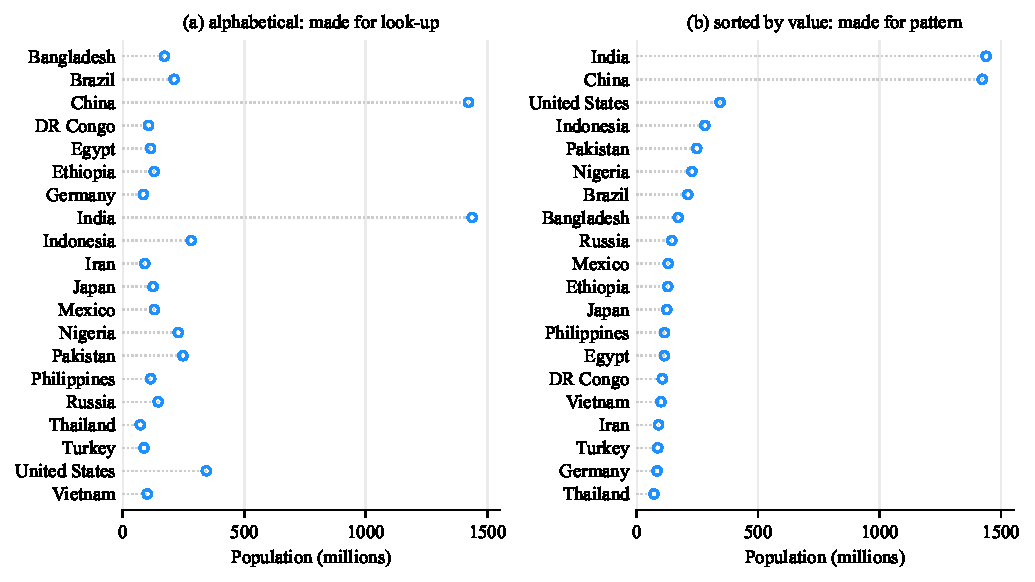
\includegraphics{plot_lookup}
	\caption{The populations of the 20 most populated countries, drawn twice with nothing changed but the order of the rows. (a) Alphabetical: Country is found in one jump, and the distribution of populations has to be assembled row by row. (b) Sorted by value; country now costs a scan of up to twenty rows. 
	\footnotesize Example after Cleveland, \emph{The Elements of Graphing Data}. Data: United Nations, \emph{World Population Prospects}, 2024 revision, mid-$2023$ estimates.}
	\label{fig-plot-lookup}
\end{figure}

Neither panel answers both questions, and the one it answers is decided by the ordering rather than by the encoding, which is identical in the two. So the ordering is not a formatting detail. Most figures in a technical document are read for pattern, which is why sorting by value is the default (Sec.~\ref{sec-app-plot-dataink}).

\begin{box_red}[Figure$\rightarrow$Table]
a figure that is genuinely consulted by name wants alphabetical order; and a figure that is only ever consulted by name wants to be a table.
\end{box_red}

\FloatBarrier
\section{Color}\label{sec-app-plot-color}

Color buys three no other channel offers at the same price: 
\begin{itemize}
	\item it calls attention to one mark among hundreds without enlarging it or moving it,
	\item it gives a figure something to be remembered by,
	\item it adds a dimension to a page that has only two.
\end{itemize}
\begin{box_blue}[Color is the easiest channel to misuse]
Colors always produce a picture and the picture always looks like data.
\end{box_blue}


\subsection{Which part of a color can be ranked}\label{sec-app-plot-colorspace}

A color in a figure is three numbers: how much red, how much green and how much blue the screen mixes. Each runs from $0$ to $1$, or equivalently from $0$ to $255$, so every color a figure can use is a point in the box of Fig.~\ref{fig-plot-rgbcube} --- black at the origin where all three are $0$, white at the opposite corner where all three are $1$, and the grays on the diagonal between them, where the three are equal.

\begin{figure}[ht]
	\centering
	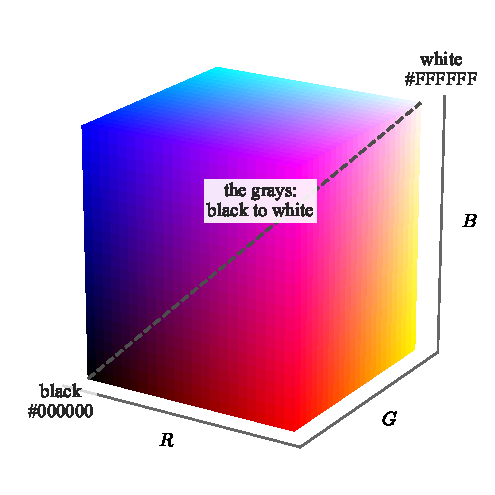
\includegraphics{plot_rgbcube}
	\caption{The RGB cube: every color a figure can use, as a point in the box of the three numbers. The eight corners are black, white and the six pure mixes; the dashed diagonal, where $R=G=B$, carries the grays from black to white. The two labeled corners give the three numbers in their usual written form.}
	\label{fig-plot-rgbcube}
\end{figure}

\begin{box_blue}[Hex codes]
	The same three numbers are almost always written as six hexadecimal digits, two per channel, running from \texttt{00} to \texttt{FF}: \texttt{\#000000} is black, \texttt{\#FFFFFF} white, \texttt{\#FF0000} red, \texttt{\#808080} mid gray, and \texttt{\#1F77B4} is the blue \texttt{matplotlib} draws its first line in. Every plotting library, style file and web page accepts this form, and it is the form in which a palette should be recorded --- a color called ``blue'' is a different color in every tool, while \texttt{\#1F77B4} is not.
\end{box_blue}

Two colors written that way are two points in the cube, so how far apart they are is the straight line between them,
\begin{equation}
	d = \sqrt{(R_1-R_2)^2 + (G_1-G_2)^2 + (B_1-B_2)^2} ,
	\label{eq-plot-rgb-distance}
\end{equation}
with $d=0$ for one color written twice and, at the other extreme, $d=\sqrt{3}\approx1.73$ for black against white, the diagonal of the cube. Equal steps of $d$ are not equally visible, so it is a poor measure of \textit{how} different two colors look. What it does answer is whether they are distinct at all, which is what a palette of several colors has to guarantee.

What a figure keeps when it is printed in black and white is computable from the three numbers, $g = 0.21R + 0.72G + 0.07B$, with $g=0$ for black and $g=1$ for white. It is called the \emph{gray level} here. The approximation is the quantity of interest, because it is what a black-and-white printer or a photocopier actually delivers.

\begin{box_yellow}[Print it in gray]
	Any figure may be printed in black and white, projected badly, or photocopied. \emph{Test} a figure in gray, not draw it in gray.
\end{box_yellow}

\begin{box_yellow}[Dark-to-light ranking]
Only dark-to-light can be ranked. Darker and lighter form a scale a reader orders without being told the rule.
\end{box_yellow}
Fig.~\ref{fig-plot-colorsort} is what that sentence means operationally. Eight values are encoded dark to light and shown three times: shuffled, in their true order, and as the gray a black-and-white print would keep.

\begin{figure}[ht]
	\centering
	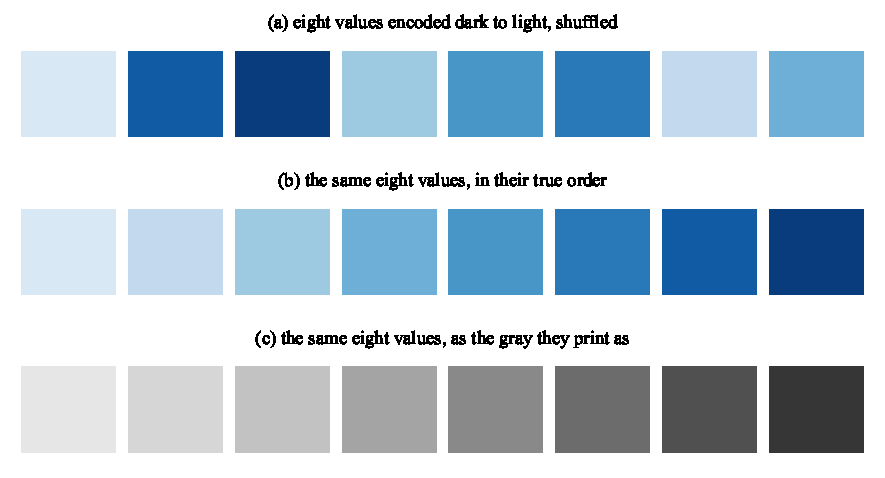
\includegraphics{plot_colorsort}
	\caption{Eight values encoded dark to light. (a) Shuffled: the row can be put back in order by eye, without being told which end is large. (b) The true order. (c) The same eight values as the gray a black-and-white print keeps, falling steadily from $0.90$ to $0.21$. Sorting on that gray level recovers the true order exactly, which is the same operation the reader performs in (a).}
	\label{fig-plot-colorsort}
\end{figure}

An ordered quantity therefore needs an ordered channel. If the reader must rank, compare or interpolate, the value has to move the marks from dark to light; if the reader must only tell one thing from another, a different color is exactly the right answer.

\subsection{Color and grayscale are judged in context}\label{sec-app-plot-context}

The eye does not measure a color, it compares one. Every patch is reported relative to what surrounds it, so the same ink can be read as two different quantities in two places on the same page. Fig.~\ref{fig-plot-graycontrast} is the demonstration, and it uses no color at all.

\begin{figure}[ht]
	\centering
	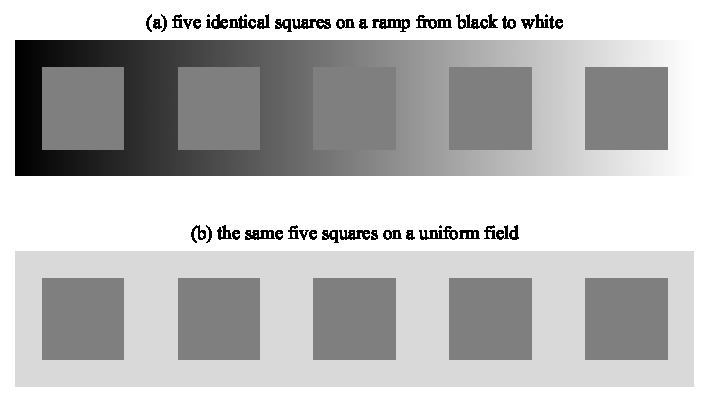
\includegraphics{plot_graycontrast}
	\caption{Gray in context. (a) Five squares, every one of them painted the identical $\mathrm{RGB}=(0.50,0.50,0.50)$, placed along a ramp running from black to white. They appear to darken steadily from left to right, and the third square, which sits exactly where the ramp reaches its own value, disappears. (b) The same five squares on a uniform field, where they are visibly one color; the only thing that differed between them in (a) is what lay behind them, which runs from $0.10$ to $0.90$.}
	\label{fig-plot-graycontrast}
\end{figure}

\begin{box_blue}
	Gray is a poor default rather than a safe one (Fig.~\ref{fig-plot-graycontrast}).
\end{box_blue}
\begin{box_yellow}
	A shade is only comparable to another shade on the same background.
\end{box_yellow}


\subsection{Colormaps}
\begin{goal}
	What color for this number?
\end{goal}
\begin{box_blue}[Colormap]
	A \emph{colormap} is a function from a scalar to a color, $m:[0,1]\to(R,G,B)$, applied after the data has been normalized onto $[0,1]$.
\end{box_blue}

What separates one colormap from another is how the gray level $g$ of Sec.~\ref{sec-app-plot-colorspace} runs along the map, from one end to the other, and the requirement follows from what the map is being asked to encode. A sequential map has to get lighter throughout, because the reader must be able to rank any two values it produces. A diverging map has to turn exactly once, at the value its center is pinned to, which is what makes it read as a distance from that center. A map that turns anywhere else puts an edge on the page where the data has none. Fig.~\ref{fig-plot-cmap-gray} shows four maps against that requirement.

\begin{figure}[ht]
	\centering
	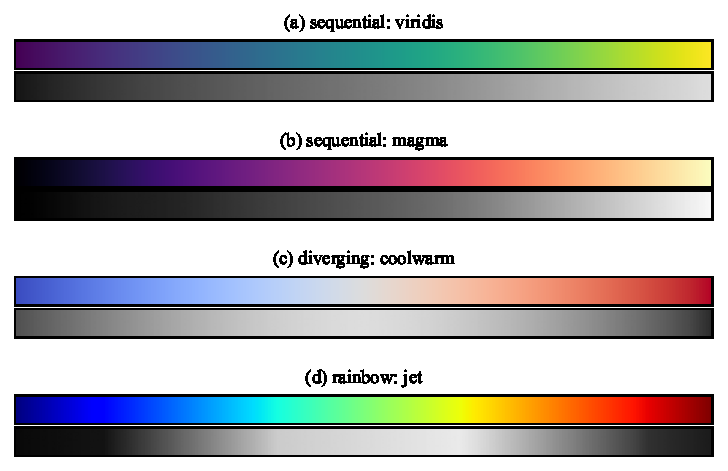
\includegraphics{plot_cmap_gray}
	\caption{Four colormaps, each as the reader sees it and as the gray it prints as. (a) \texttt{viridis} and (b) \texttt{magma} get lighter throughout, over $0.08$ to $0.87$ and $0.00$ to $0.97$, so either can carry a magnitude. (c) \texttt{coolwarm} is lightest in the middle and darkens to both ends, which is the center it is built around and not a fault. (d) \texttt{jet} covers $0.04$ to $0.92$ and does neither: it is lightest near the middle, dark at both ends, and reverses on the way.}
	\label{fig-plot-cmap-gray}
\end{figure}

The gray rows are hard to compare bar against bar, so Fig.~\ref{fig-plot-cmap-curve} draws the same four gray levels as curves, one against the other.

\begin{figure}[ht]
	\centering
	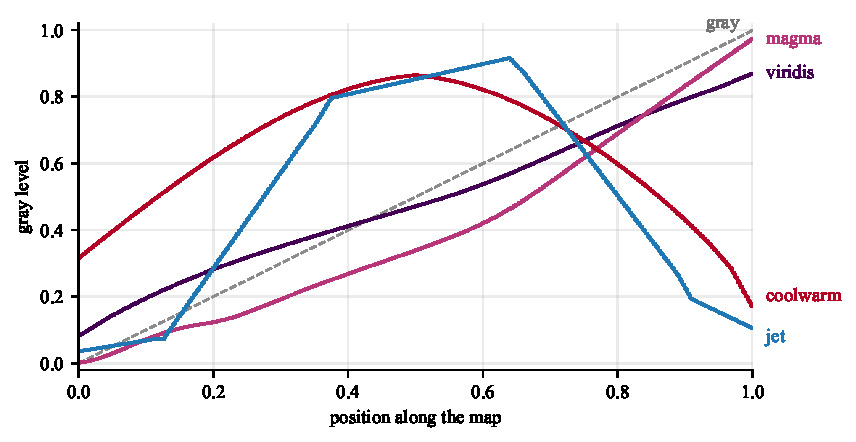
\includegraphics{plot_cmap_curve}
	\caption{The gray level of the four maps of Fig.~\ref{fig-plot-cmap-gray}, against position along the map, with the \texttt{gray} map itself as the dashed straight line. \texttt{viridis} and \texttt{magma} climb without turning. \texttt{coolwarm} turns once, at position $0.50$. \texttt{jet} turns three times, the last at $0.64$, after which it darkens again toward its own maximum. The steps are also uneven, measured as $\mathrm{std}\lvert\Delta g\rvert / \mathrm{mean}\lvert\Delta g\rvert$ along the map: $0.20$ for \texttt{viridis} against $0.69$ for \texttt{jet}, so equal steps in the data do not arrive as equal steps of gray on the page.}
	\label{fig-plot-cmap-curve}
\end{figure}

The rainbow colormaps, of which \texttt{jet} is the most common, fail this test outright. Fig.~\ref{fig-plot-colormap} shows what the failure does to a field, by reducing each map to the gray it prints as.

\begin{figure}[ht]
	\centering
	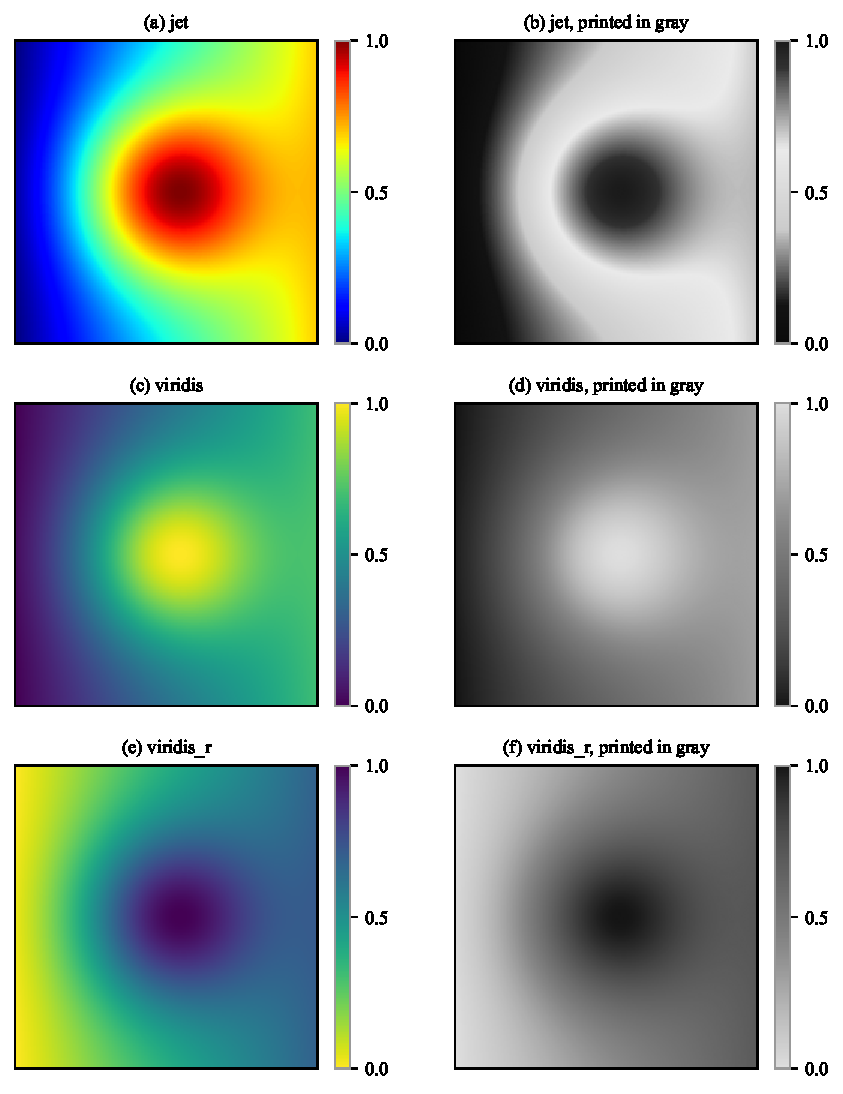
\includegraphics{plot_colormap}
	\caption{Three colormaps, each shown in color and as the gray a black-and-white print leaves. (a) and (b): \texttt{jet}, turns around three times on the way, so the peak comes out \textit{dark} and a bright false ring appears around it. (c) and (d): \texttt{viridis}, which only ever gets lighter over the same range. (e) and (f): \texttt{viridis\_r}, the same map run backwards, which never stops getting \emph{darker} and is therefore just as rankable, with the peak now the darkest ink on the page. Every panel carries its own colorbar, over a field normalized to $[0,1]$, and the bar of a gray panel is the gray that map prints as: the bar of (b) is dark at both ends and light in the middle, where those of (d) and (f) run one way from end to end.}
	\label{fig-plot-colormap}
\end{figure}

The dark blob in Fig.~\ref{fig-plot-colormap}(b) is at the maximum of the field. That inversion, and the bright ring the eye reads as a boundary, are artifacts of the colormap, not features of the data. A map such as \texttt{viridis}, \texttt{magma} or \texttt{cividis} avoids them by construction: it is built so that equal steps in the data look like equal steps to the reader, and so that it never stops getting lighter.

\paragraph{\texttt{jet} colormap}
Why, then, is it still everywhere? Almost never because anyone chose it. 
\begin{itemize}
	\item Was the MATLAB default until R2014b and the \texttt{matplotlib} default until version~2.0, so every script and every figure written before those releases is \texttt{jet} by omission, and copied code carries the choice forward without ever restating it.
	\item Instrument software keeps it alive on its own: spectrum analyzers, thermal cameras, Doppler ultrasound, and seismic and weather displays ship it, often with no setting to change it.
	\item When a field has trained its readers on a fixed color-to-meaning mapping, or a figure must sit beside an archive drawn the same way, changing the map breaks the comparison the figure exists to support.
	\item The three turns of Fig.~\ref{fig-plot-cmap-curve} put visible bands and edges on the image, and in color, at full brightness, that extra structure reads as detail rather than as damage; the author sees a sharp picture, and only the reader of the printed version sees Fig.~\ref{fig-plot-colormap}(b).
	\item Color also names a value well even though it ranks values badly. ``The red region'' is easy to say and easy to match against a colorbar, so reading one value off the figure feels accurate.
\end{itemize}

\begin{box_blue}[Inherited, not chosen]
	\texttt{jet} on a figure is almost always a default nobody revisited. Change it, unless the figure has to be read against an archive drawn the same way, and (optionaly) say so in the caption.
\end{box_blue}
\FloatBarrier

\subsection{Schemes}\label{sec-app-plot-colormap-scheme}
\begin{goal}
Which colors for these categories?
\end{goal}
\begin{box_blue}[Scheme]
	A \emph{scheme}, or \emph{palette}, is a short fixed list of colors chosen as a set, $\{c_1,\dots,c_k\}$. 
\end{box_blue}
Colormaps and schemes are convertible, which is why the words get swapped: sampling a colormap at $k$ points produces a scheme, and interpolating between the entries of a scheme produces a colormap. The first direction is routine for the ordered families below, and is how most sequential schemes are obtained. The second is not, because interpolating between unordered categories produces colors that stand for nothing.

\subsubsection{Choosing a scheme}
\begin{itemize}
	\item \emph{Sequential}, one color running light to dark, for a quantity with a low end and a high end: counts, magnitudes, probabilities, densities. Its $k$ colors are a sequential colormap cut into $k$ classes.
	\item \emph{Diverging}, two colors meeting at a neutral middle, for a quantity with a meaningful center: residuals and errors around zero, correlations, differences between two models. The middle must be pinned to the meaningful value, or the map asserts a center where none exists.
	\item \emph{Qualitative}, different colors of similar darkness, for unordered categories: class labels, model names, cluster identities. Six to eight is the practical ceiling; past that, the colors stop being distinguishable and direct labeling is the answer.
\end{itemize}

An excellent source of schemes is Cynthia Brewer's picker at \url{https://colorbrewer2.org}, most of which ships with \texttt{matplotlib} under the same names.\footnote{M.~Harrower and C.~A.~Brewer, \href{https://doi.org/10.1179/000870403235002042}{``ColorBrewer.org: An Online Tool for Selecting Colour Schemes for Maps''}, \emph{The Cartographic Journal}, vol.~40, no.~1, 2003, pp.~27--37. The tool also filters on colorblind-safe, print-safe and photocopy-safe, which is the check of Sec.~\ref{sec-app-plot-checks} applied before the figure exists rather than after.}

Fig.~\ref{fig-plot-schemes} shows two schemes from each family with its gray beneath, which turns the choice from a matter of taste into a matter of shape.

\begin{figure}[ht]
	\centering
	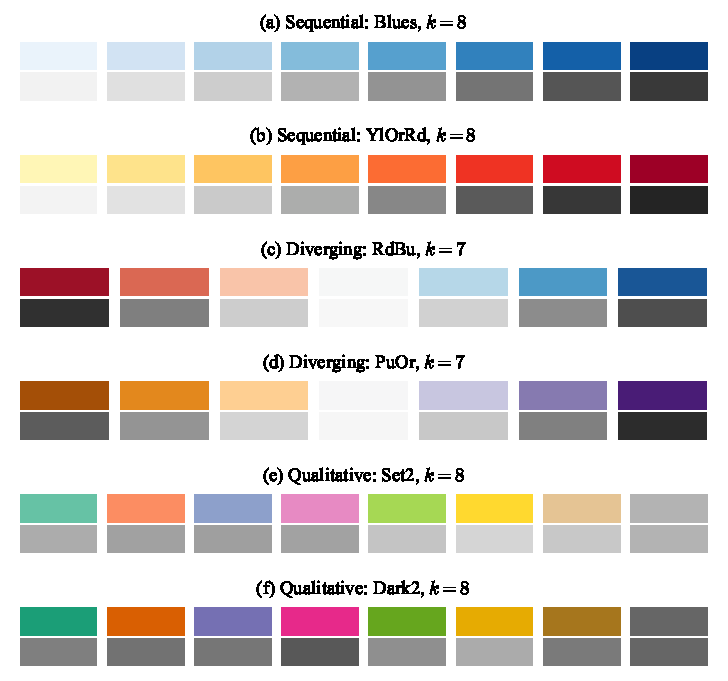
\includegraphics{plot_schemes}
	\caption{Two ColorBrewer schemes from each family, each drawn as the $k$ fixed colors it is, in color and as the gray it prints as. (a) and (b) Sequential, $k=8$: the gray only ever moves one way. (c) and (d) Diverging, $k=7$, an odd count so that the neutral class is a color of its own rather than a boundary between two: the gray is lightest at that middle class, at position $0.50$ of the map in both, and darkens to both ends, so the scheme reads as a distance from a center. (e) and (f) Qualitative, $k=8$: the gray is deliberately almost flat, so the categories separate by color and none of them looks larger than another.}
	\label{fig-plot-schemes}
\end{figure}

The gray rows also say what each family must not be used for. A sequential map has no center to put a zero on; a diverging map applied to a quantity with no meaningful center asserts one; and a qualitative map used for a magnitude leaves the reader nothing to rank with.

\FloatBarrier
\subsection{Color deficiency}\label{sec-app-plot-checks}
The deficiency is not one condition. Fig.~\ref{fig-plot-cvd-types} passes the visible spectrum through each common form, and Table~\ref{tab-plot-cvd} gives how frequent each one is. 

\begin{figure}[h]
	\centering
	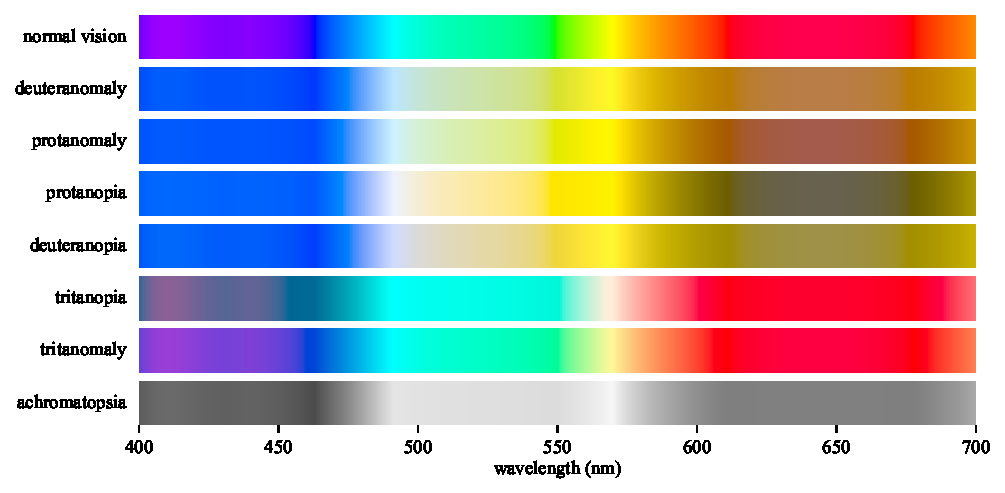
\includegraphics{plot_cvd_types}
	\caption{The visible spectrum as each common form of color vision deficiency receives it. The bar approximates the spectrum and is not a colorimetric reference.}
	\label{fig-plot-cvd-types}
\end{figure}

\begin{table}[h]
	\centering
	\caption{How common each form is, among people of Northern European ancestry, in the row order of Fig.~\ref{fig-plot-cvd-types}. The red-green forms of the first four rows reach about $8\%$ of men, two orders of magnitude above the blue-yellow forms below them.}
	\label{tab-plot-cvd}
	\begin{tabular}{L{5cm}|R{1.2cm}@{}L{1.8cm}|R{1.2cm}@{}L{1.8cm}}
		\toprule
		Form & \multicolumn{2}{C{3cm}|}{Men} & \multicolumn{2}{C{3cm}}{Women} \\
		\midrule
		Deuteranomaly & 5 & \% & 0 & .35\% \\
		Protanomaly & 1 & .3\% & 0 & .02\% \\
		Protanopia & 1 & .3\% & 0 & .02\% \\
		Deuteranopia & 1 & .2\% & 0 & .01\% \\
		Tritanopia & 0 & .008\% & 0 & .008\% \\
		Tritanomaly & 0 & .0001\% & 0 & .0001\% \\
		\bottomrule
	\end{tabular}
\end{table}

\begin{box_red}[Red-green pair]
Never let a \textbf{red-green pair} be the only thing separating two series.
	
Red-green deficiency affects roughly $8\%$ of men of Northern European ancestry and $0.4\%$ of women.
\end{box_red}
\FloatBarrier

Fig.~\ref{fig-plot-cvd} runs the same simulation on one chart drawn with two palettes.\footnote{Both figures simulate deficiency after Machado, Oliveira and Fernandes, \href{https://doi.org/10.1109/TVCG.2009.113}{``A Physiologically-based Model for Simulation of Color Vision Deficiency''}, \emph{IEEE Trans.\ Visualization and Computer Graphics}, vol.~15, no.~6, 2009, pp.~1291--1298. In Fig.~\ref{fig-plot-cvd} it is applied to the rendered pixels of the chart, so the legend keys degrade exactly as the lines do. Fig.~\ref{fig-plot-cvd-types} redraws \href{https://commons.wikimedia.org/wiki/File:Color_blindness.svg}{``Color blindness''} by SyntaxTerror, Public domain, via Wikimedia Commons, and Table~\ref{tab-plot-cvd} follows the epidemiology table of Wikipedia contributors, \href{https://en.wikipedia.org/w/index.php?title=Color_blindness\&oldid=1368875735}{``Color blindness''}, \emph{Wikipedia, The Free Encyclopedia}, revision of 11~August 2026, retrieved 18~August 2026.} The data, the layout and the legend are identical in the two rows, so whatever separates them is the palette alone.

\begin{figure}[ht]
	\centering
	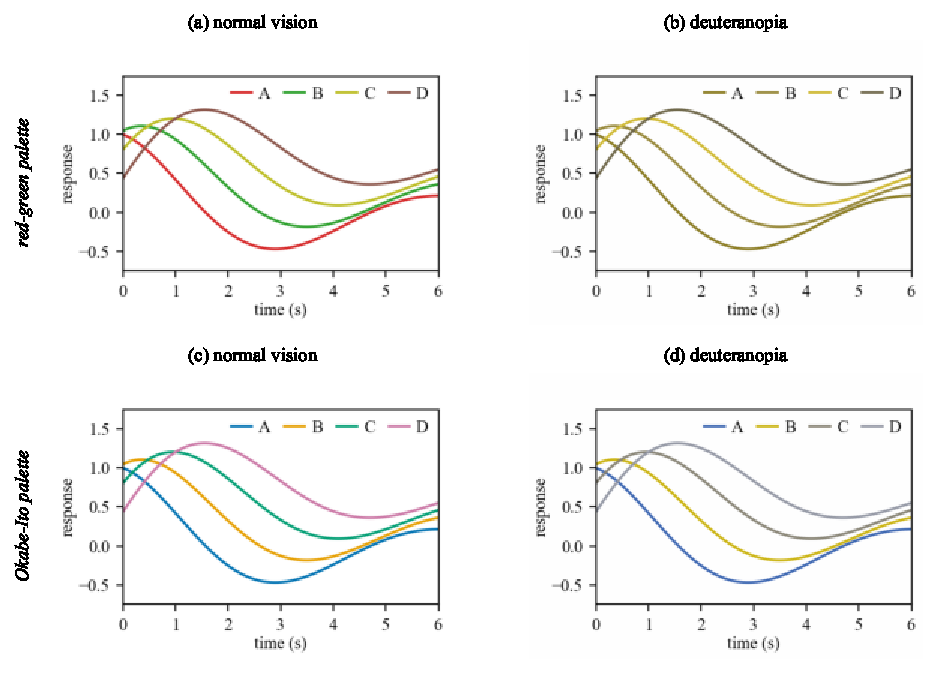
\includegraphics{plot_cvd}
	\caption{One four-series chart under two palettes, each shown in normal vision and under simulated deuteranopia. (c) \textit{Okabe-Ito} palette. (d) all four series stay separable.}
	\label{fig-plot-cvd}
\end{figure}

The palette of the lower row is not an invention of that figure. Fig.~\ref{fig-plot-okabeito} gives it in full: eight colors chosen so that no two of them merge under any common form of deficiency, published with a name and a code for each so that a figure can be specified in them.

\begin{figure}[ht]
	\centering
	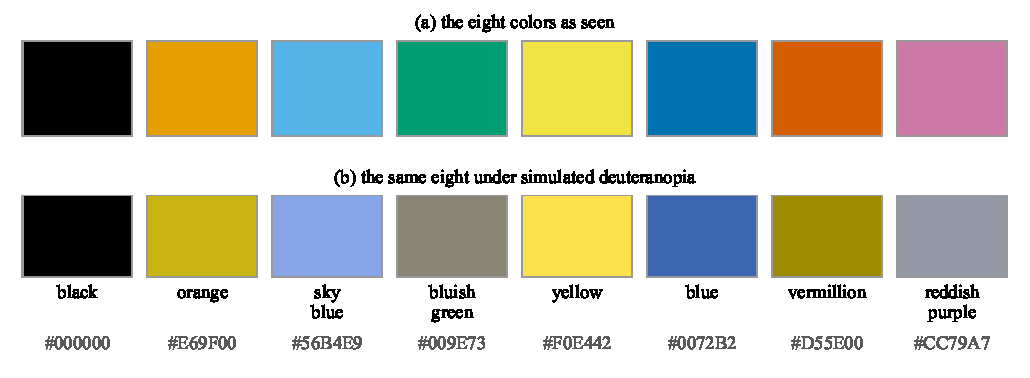
\includegraphics{plot_okabeito}
	\caption{The Okabe-Ito qualitative palette, with the name and the hex code of every color. (a) As seen. (b) The same eight under simulated deuteranopia. The closest pair of (a), orange and vermillion, separates by $0.263$ in RGB; the closest pair of (b), bluish green and reddish purple, still separates by $0.202$, so the eight stay tellable apart. Source: Okabe and Ito, \emph{Color Universal Design} (2008), tabulated in Wong (2011).}
	\label{fig-plot-okabeito}
\end{figure}

\begin{box_yellow}[Okabe-Ito]
	Eight colors that survive every common deficiency, in the order they are published: \texttt{\#000000}, \texttt{\#E69F00}, \texttt{\#56B4E9}, \texttt{\#009E73}, \texttt{\#F0E442}, \texttt{\#0072B2}, \texttt{\#D55E00}, \texttt{\#CC79A7}. Take them in that order and stop when the figure has enough; four of them are Fig.~\ref{fig-plot-cvd}(c).
\end{box_yellow}

A figure that survives \textit{both} black and white print and vision deficiency simulation is legible to almost everyone. 

\begin{box_yellow}[Double encoding]
	Use \textit{double encoding} whenever a distinction matters: give the series different:
	\begin{itemize}
		\item line styles or markers,
		\item colors.
	\end{itemize} 
\end{box_yellow}
\FloatBarrier

\subsection{Color Meaning}\label{sec-app-plot-meaning}
\subsubsection{Social aspects}
Finally, color carries meaning that the data may not intend. Red reads as loss, danger or failure and green as the opposite, and the reader applies that mapping before reading the axis. A figure that assigns the colors the other way is not merely unhelpful, it is asserting something about every mark on the page that the numbers contradict. Fig.~\ref{fig-plot-semantic} puts one record through both assignments.

\begin{figure}[ht]
	\centering
	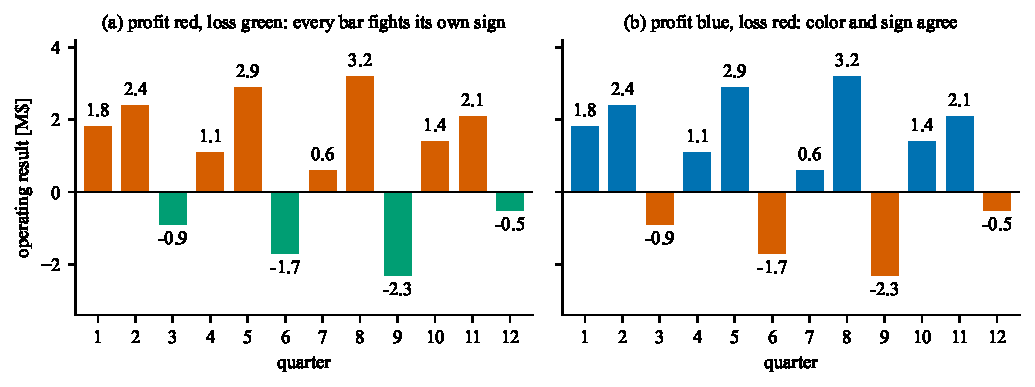
\includegraphics{plot_semantic}
	\caption{Twelve quarters of an operating result, drawn twice from the same numbers on the same zero baseline. 
		(a) Profit in red and loss in green: all $12$ bars carry a color that contradicts their own sign, $8$ profits in red and $4$ losses in green, and the reader has to override the color on every one of them. (b) Profit in blue and loss in red, where none does. The positive side is blue rather than green because \textit{red-green} is the pair that roughly $8\%$ of men cannot separate (Sec.~\ref{sec-app-plot-checks}), so only the negative side keeps the conventional red.}
	\label{fig-plot-semantic}
\end{figure}

\subsubsection{One strong color}
Strong color is a budget. Spend it on the one series, region or mark the text is about, draw everything else in gray at $20$ to $40\%$ ink, and let the reader find the subject pre-attentively, by the mechanism of Fig.~\ref{fig-plot-preattentive}, without being told where to look.  Fig.~\ref{fig-plot-highlight} spends the budget both ways.

\begin{figure}[h]
	\centering
	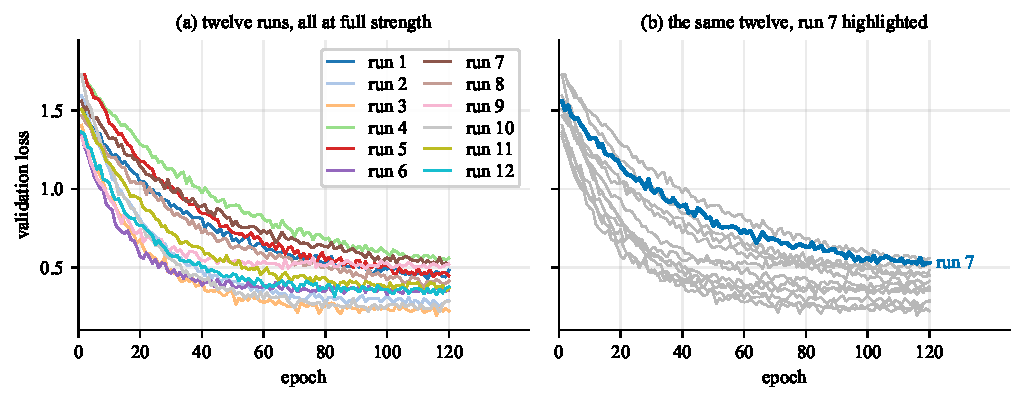
\includegraphics{plot_highlight}
	\caption{Twelve validation curves on identical axes. (a) All twelve at full strength, and $12$ legend keys are needed to name them. (b) Eleven dropped to gray $0.72$, which is $28\%$ ink, against one at $0.37$, or $63\%$ ink: a contrast of $0.35$ that makes the highlighted curve the only thing the eye lands on. It is named at its own end, so the panel needs no key at all.}
	\label{fig-plot-highlight}
\end{figure}
\FloatBarrier

\section{Choosing the Encoding}\label{sec-app-plot-encoding}
A chart maps numbers onto a visual channel, and the channels are not interchangeable. Their accuracy has been measured. The ranking is stable, and it is the most useful result in the field:

\begin{enumerate}
	\item position along a common scale;
	\item length;
	\item slope and angle;
	\item area;
	\item volume;
	\item shading and color strength;
	\item a different color.
\end{enumerate}

Fig.~\ref{fig-plot-encoding} puts one set of five values through the first six of these channels, one panel per entry, from panel~(a) for the first to panel~(f) for the sixth, so the ranking can be felt rather than taken on trust. The seventh has no panel here because it has no answer: a set of colors is a set of names, and names do not come in an order, so the ranking cannot be recovered at all. Only the dark-to-light part of a color can be ranked, which is the subject of Sec.~\ref{sec-app-plot-colorspace}.

\begin{figure}[ht]
	\centering
	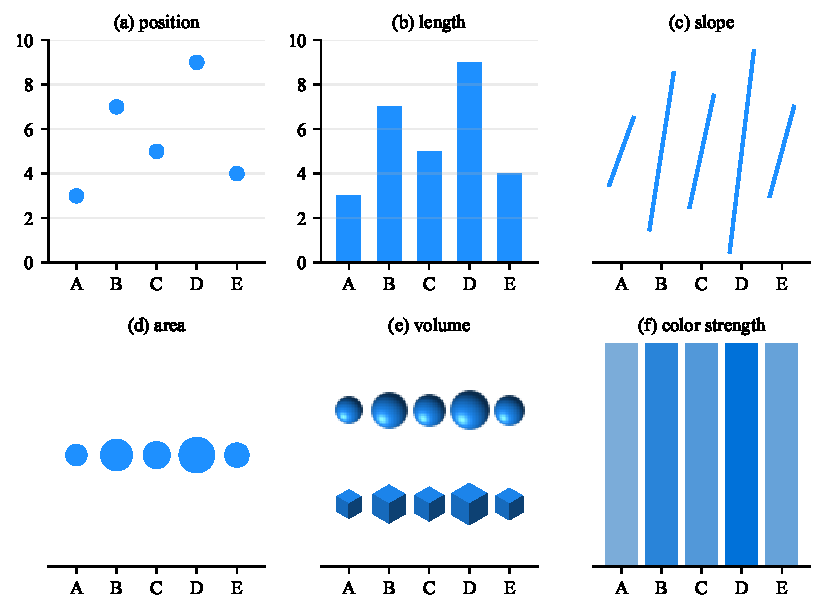
\includegraphics{plot_encoding}
	\caption{Five values, $A$ to $E$, encoded six ways, one panel per entry of the ranking above. Rank the categories from smallest to largest in each panel. The answer is $A < E < C < B < D$ throughout. Panels (a) and (b) give it up immediately. Panels (c) to (e) take effort and invite errors between the close pair $B$ and $C$, and the two size channels differ in how much of the difference survives: $D$ is three times $A$, and its mark has three times the area in (d) and only $2.1$ times in (e), where the value is a volume, so the radius of the ball and the edge of the cube both follow its cube root. Panel~(f) cannot be done reliably at all.}
	\label{fig-plot-encoding}
\end{figure}

Three consequences follow, and they account for most of the chart-type advice in circulation.

\begin{box_yellow}[Bar, line and scatter]
Bar, line and scatter are the workhorses. They occupy the top of the ranking. There is rarely a reason to reach past them for quantitative data.
\end{box_yellow}

\FloatBarrier
\subsection{Case Study: Pie and 3D plots}\label{sec-app-plot-pie}
\paragraph{Pie charts encode angle and area}
Both sit low in the ranking, which is why comparing two slices of similar size is guesswork, and why a pie with more than three slices cannot be ordered by eye. The same numbers as a sorted bar chart are read exactly, in the same space. 

\paragraph{Three dimensions on a flat page cost accuracy and buy nothing}
A 3D bar chart replaces length, which is second in the ranking, with volume under projection, which is fifth, and adds occlusion so that some bars hide others. Adding perspective makes it worse than guesswork: tilting the pie shrinks the back slices and enlarges the front ones, so the picture is no longer even a faithful rendering of the angles.

Both paragraphs above can be checked on one set of numbers. Fig.~\ref{fig-plot-pie} takes the five values $37$, $36$, $24$, $2$ and $1$ through the four charts a spreadsheet offers for them. The two largest differ by one part in a hundred, and that difference is the test: every panel contains it, and one panel shows it.

\begin{figure}[ht]
	\centering
	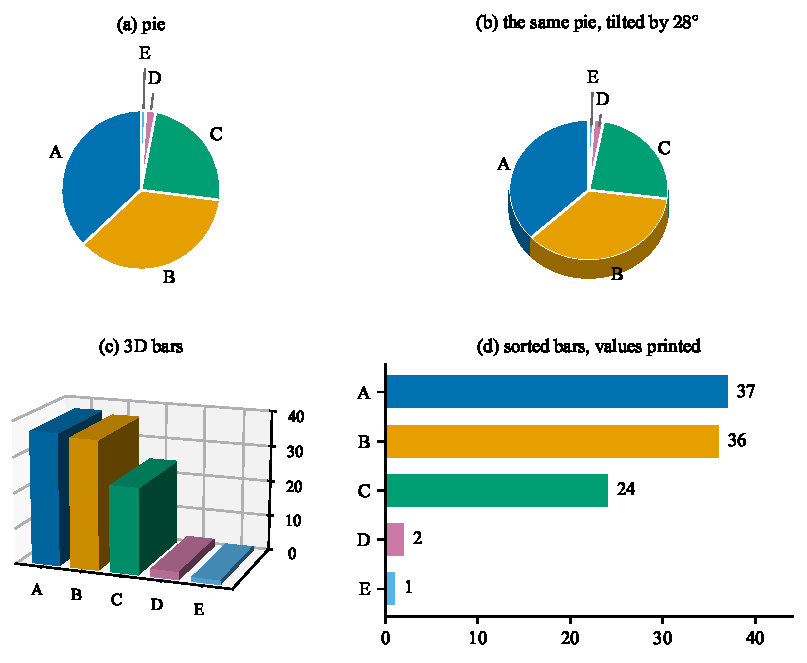
\includegraphics{plot_pie}
	\caption{Five values, $A=37$, $B=36$, $C=24$, $D=2$, $E=1$, drawn four ways. (a) A pie: $A$ and $B$ differ by $3.6^{\circ}$ of arc out of $360^{\circ}$, so the two cannot be ordered, and the slivers $D$ and $E$ need leaders to be labeled at all. (b) The same pie tilted by $28^{\circ}$: $B$ lies at the front and collects the slab wall, so it is drawn with $1.27$ times the apparent area of $A$ although it is the smaller value. (c) The same values as 3D bars: the front bar tops reads between $7$ and $11$ units low, which distorts the differences as well as the values. (d) Sorted bars with the values printed: the ranking is immediate and the numbers are exact.}
	\label{fig-plot-pie}
\end{figure}

Panel~(d) is not a more careful version of the others, it is a different encoding. It reads the values as length from a common baseline, second in the ranking, while (a) and (b) read them as angle and area, third and fourth, and (c) reads them as a height that has to be carried across a gap in depth before it meets a scale. 

\FloatBarrier
\subsection{Case Study: Three variables on a flat page}\label{sec-app-plot-thirdvar}

Two variables get the two axes. A third has to go into a channel, and which channel is the whole question, because the ranking above is the answer to it. Fig.~\ref{fig-plot-thirdvar} takes one record of forty training runs, each with a model size, a training set size and the accuracy it reached, and moves the training set size through four channels, one per panel. The reader is meant to take off the page that model size stops paying past about ten million parameters and training set size does not, so which of the two is worth the next budget.

\begin{figure}[ht]
	\centering
	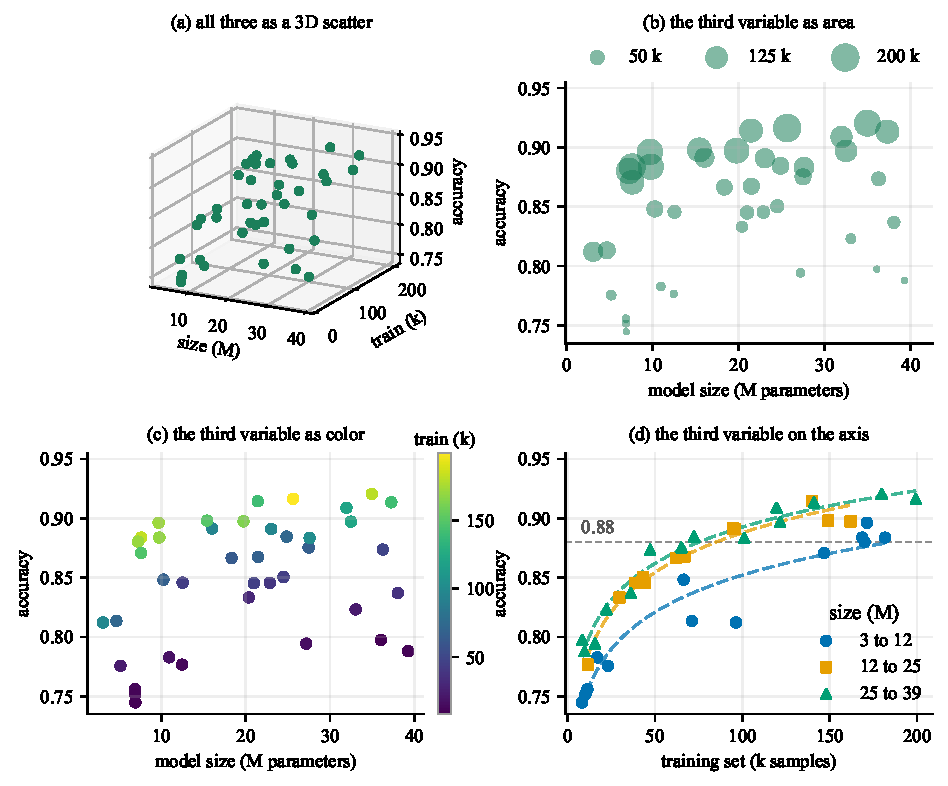
\includegraphics{plot_thirdvar}
	\caption{Three variables. (a) All three as a 3D scatter. (b) The training set as marker area. (c) The training set as color, on \texttt{viridis} with a colorbar. (d) The training set on the horizontal axis, model size as three bins in color (Okabe-Ito scheme) and marker shape at once. }
	\label{fig-plot-thirdvar}
\end{figure}

The four panels are four entries of the ranking, and they come out in its order. 
\begin{itemize}
	\item Panel~(a) is not on the ranking at all: a projected point has no depth to decode, which is the argument of Sec.~\ref{sec-app-plot-pie} moved from a pie to a scatter.
	\item Panel~(b) reads it as area, fourth.
	\item Panel~(c) reads it as color strength, sixth, which supports \textit{more} and \textit{less} and stops there. 
	\item Panel~(d) reads the third variable as position on a common scale, first, which is why the number the question turns on is read off an axis instead of estimated.
\end{itemize}
Note (d) carries model size in two channels at once, color and marker shape. 

\FloatBarrier
\subsection{Case Study: Radar charts}\label{sec-app-plot-radar}

\begin{box_blue}[Radar chart]
	A \emph{radar chart}, also called a spider or a web chart, places $k$ categories at $k$ equally spaced angles, draws each value as a radius along its own spoke, and joins the ends into a closed polygon. The angle is a \textit{slot} rather than a quantity, which is what separates it from a polar plot: there the angle carries a direction, a phase or a time of day, and none of what follows applies.
\end{box_blue}

The form has one honest use and it is narrow: a small number of profiles, measured on axes that genuinely share a scale, read for their shape rather than for their values. Every attribute is scored by the same panel on the same scale, so the radial axis means one thing on every spoke. Fig.~\ref{fig-plot-radar} takes one such record, four samples scored on six attributes, draws it in the form the chart usually takes, and measures beside it what that form does to the levels.

\begin{figure}[ht]
	\centering
	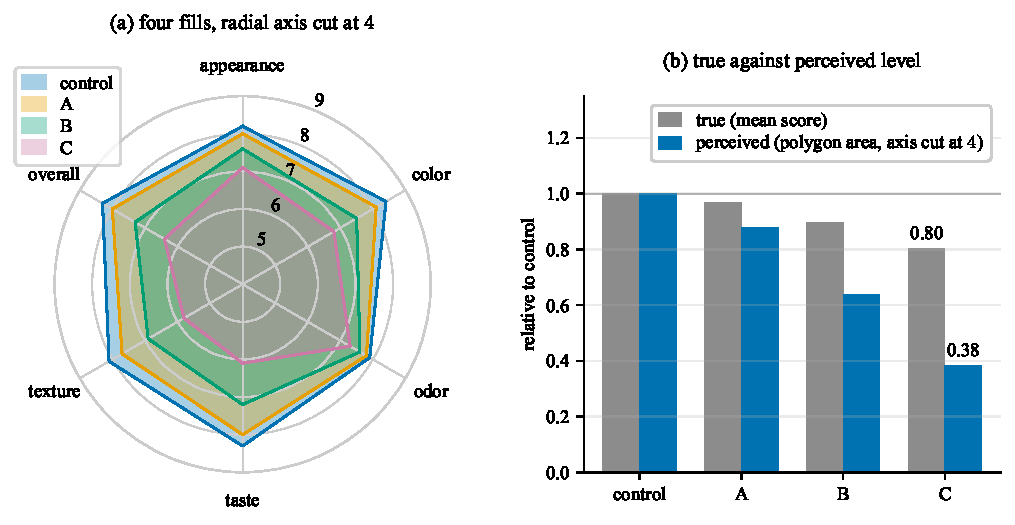
\includegraphics{plot_radar}
	\caption{One synthetic sensory record: four samples, six attributes, every attribute scored on the same $9$-point scale, drawn as a radar chart and measured against it. (a) All four filled at $\alpha = 0.35$ on a radial axis starting at $4$. The cut removes the inner $44\,\%$ of every radius and takes the apparent area of sample C; the fills occlude one another in the order they were drawn. (b) The cost of that encoding, as a length: for each sample, the true level, its mean score relative to the control, beside the level the polygon area of panel~(a) makes the reader perceive, both on a zero baseline.}
	\label{fig-plot-radar}
\end{figure}

Panel~(b) measures what panel~(a) costs. The gray bar is what a sample scored, the blue bar is the level its polygon in panel~(a) makes the reader perceive. The gap between the two is contributed by the encoding rather than by the data: nothing on panel~(a) discloses that they differ. The gap widens with the drop, from $0.09$ for sample A to $0.42$ for sample C, so the chart is least trustworthy exactly where the finding is.

What panel~(a) does wrong follows from what the polygon is. Its area on $k$ equally spaced spokes with radii $r_1,\dots,r_k$ is
\begin{equation}
	A_{\mathrm{poly}} = \frac{1}{2}\sin\!\left(\frac{2\pi}{k}\right)\sum_{i=1}^{k} r_i\,r_{i+1},
	\qquad r_{k+1} = r_1 ,
	\label{eq-plot-radar-area}
\end{equation}
and two properties of that expression decide how the chart reads.

\emph{The area is quadratic in the values.} The eye compares the filled shapes and not the radii. Sample C scores $0.803$ of the control level and its polygon covers $0.646$ of the control area, which overstates the drop by a factor of $1.80$; that comparison is the pair of bars panel~(b) draws. That is the exaggeration of a cut bar chart (Sec.~\ref{sec-app-plot-axes}) in a form no axis label discloses.

\emph{The area depends on the order of the spokes.} Eq.~\eqref{eq-plot-radar-area} pairs adjacent radii only, so permuting the axes changes it without changing a number. On this record the effect is small. The ordering is a choice the author makes and the reader cannot see.

The fix for panel~(a) is not a better radar chart. The same $24$ numbers as a dot plot, one row per attribute and one marker per sample on a shared horizontal scale, drawn in Fig.~\ref{fig-plot-radar-good}(b), put all of them at the top of the ranking of Sec.~\ref{sec-app-plot-encoding}: the largest difference in the record, $2.3$ points of texture between the control and sample~C, becomes a length rather than a shape. It also settles the comparison the radar chart cannot serve at all. Two attributes of one sample sit on one scale in a dot plot; on a radar chart they sit in two different directions.

\begin{box_yellow}[If you draw one]
	One zero-anchored scale on every spoke, and name it. Two profiles at most, or one per panel as small multiples (Sec.~\ref{sec-app-plot-many}). Fill one polygon or none. And say what fixes the axis order, because Eq.~\eqref{eq-plot-radar-area} says the picture depends on it.
\end{box_yellow}

Fig.~\ref{fig-plot-radar-good}(a) is that box applied to the record of Fig.~\ref{fig-plot-radar}, and panel~(b) is the dot plot beside it. Panel~(a) is as good as the form gets, and it is still the weaker of the two. Anchoring the radial axis at zero fixes the baseline and nothing else: by Eq.~\eqref{eq-plot-radar-area} the area stays quadratic in the scores, so sample~C keeps $0.803$ of the control level and $0.646$ of the area, the same factor of $1.80$ as before; the spoke order still moves the picture; and the finding of the record is a difference between two radii in (a) where panel~(b) makes it a length on one scale.

\begin{figure}[ht]
	\centering
	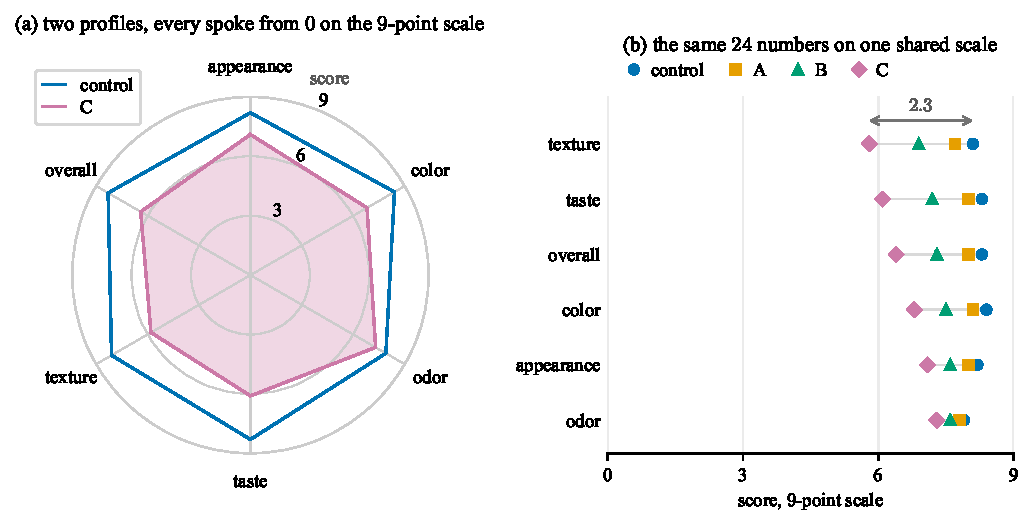
\includegraphics{plot_radar_good}
	\caption{The record of Fig.~\ref{fig-plot-radar}, drawn under the rules of the box and then not drawn as a radar chart at all. (a) Two profiles rather than four, every spoke starting at $0$ on the named $9$-point scale, one polygon filled, and the spokes in the order the questionnaire asks them, which is the order that is not chosen for how the polygon comes out. (b) The same $24$ numbers as a dot plot, one row per attribute, sorted by the gap against the control, the sample carried by color and marker shape at once so that the panel survives a gray print and a deficiency simulation (Sec.~\ref{sec-app-plot-checks}). The finding, $2.3$ points of texture between the control and sample~C, is the arrow in (b) and a comparison of two directions in (a).}
	\label{fig-plot-radar-good}
\end{figure}

\begin{box_red}[Do not normalize the axes into agreement]
Do not normalize the axes into agreement.
\end{box_red}

\FloatBarrier
\subsection{Case Study: Plot matrix}\label{sec-app-plot-matrix}
A \emph{relation} is an $n \times n$ table whose entry $(i,j)$ describes the \textit{pair} rather than a single item: confusion matrices, correlation and distance matrices, and more.
The default rendering for all of them is a colored grid, which encodes the value as shading, sixth in the ranking above.

\begin{goal}
	Draw a relation for the comparison it was measured to make. Here cell $(i,j)$ is the accuracy of a classifier trained on channel $i$ and tested on channel $j$, and the comparison is against the target channel's own model, on the diagonal.
\end{goal}

Fig.~\ref{fig-plot-matrix-raw}(a) is the grid as its script produced it, from the single line \texttt{imshow(M, cmap='viridis', vmin=M.min(), vmax=M.max())}. The map is stretched across the observed range, $0.875$ to $0.926$, so the entire excursion from deepest purple to full yellow is $5.1$ points of accuracy, and no colorbar reports it.

\begin{box_yellow}[Colorbar]
A colormap fitted to the data range, with no colorbar to disclose it, is an error to fix.
\end{box_yellow}

\begin{box_red}[Scaling]
	\begin{itemize}
		\item \texttt{vmin=M.min()} is the cut baseline of Fig.~\ref{fig-plot-baseline}(a) moved into color: the scale is pinned to the data rather than to a meaningful zero, so every apparent difference is inflated by an amount the reader cannot detect.
	Subtract the reference before you color it!

	\item Switch the text color on the gray level of the cell rather than on the value.
	\item Do not re-encode the diagonal, which position already identifies; define every glyph, since an asterisk without a key is a legend without a key.
	\item The ordering rule of Sec.~\ref{sec-app-plot-lookup}.
	\end{itemize}
\end{box_red}

The comparison the grid is being asked to support is between each transfer and the target channel's own model, and there are two ways to make it: show that reference, or subtract it. Panels~(b) and~(c) show it. They keep the accuracies exactly as they were measured and mark each target's own model beside them, so the shortfall is a distance on the page rather than a number the script arrived at, and the level of the results survives. That level is what ch~$3$'s row is for: a model transferred into ch~$3$ is the least accurate destination of the four, $0.8772$ against $0.8928$ into ch~$2$.

\begin{figure}[ht]
	\centering
	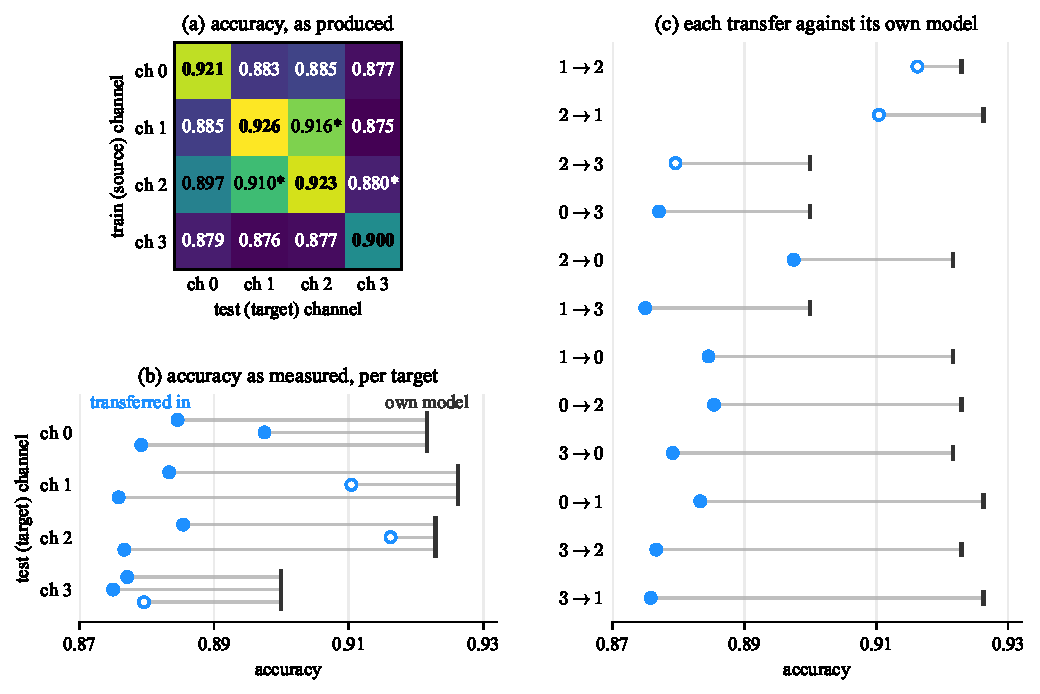
\includegraphics{plot_matrix_raw}
	\caption{One $4 \times 4$ cross-channel record, as it was measured. (a) As produced: \texttt{viridis} stretched over the observed range $0.875$ to $0.926$, no colorbar, the diagonal in bold, an unkeyed asterisk. (b) One row per target channel, three dots in it, one per model transferred in, each joined to the dark rule of that channel's own model. The segment is the loss the next figure computes, here a length on the page and nothing else. Ch~$3$'s whole row, rule included, sits left of the others. (c) The same twelve, sorted and named; the open markers are the three closest transfers. The axis is cut, which points allow and bars do not.}
	\label{fig-plot-matrix-raw}
\end{figure}

The two panels are not equally successful, and the reason is the reference. Panel~(b) draws each of the four references once, so the levels are visible as levels and ch~$3$'s rule at $0.900$, against $0.921$ to $0.926$ for the others, is the finding. Panel~(c) draws the same four references twelve times, in whatever order the sort produces; and by sorting on the segment it turns the shortfall into a length measured from twelve different starting points. Sort by a difference only when the marks that carry it start together, which is what a common zero gives and what the next figure draws.

Subtracting the reference is the other way. The quantity the argument turns on is then not the accuracy but the loss against that reference,
\begin{equation}
	\Delta_{ij} = a_{jj} - a_{ij},
	\label{eq-plot-matrix-gap}
\end{equation}
where $a_{ij}$ is the entry of the grid, the accuracy of a classifier trained on channel~$i$ and tested on channel~$j$: the row index~$i$ is the source the model was trained on, the column index~$j$ is the target it is tested on, and $a_{jj}$ on the diagonal is the target's own model, the reference every entry of column~$j$ is measured against. The loss is therefore zero on the diagonal by construction. Fig.~\ref{fig-plot-matrix}(a) draws the same numbers as $\Delta$, anchored at zero. The row reading survives, the column reading inverts: column~$3$ is the darkest of Fig.~\ref{fig-plot-matrix-raw}(a), yet its mean loss of $0.0228$ is the \textit{smallest} of the four. What is dark in that column is ch~$3$'s own model, $0.900$ against $0.921$ to $0.926$, reported by the raw matrix as though it were the effect. Ch~$3$ is at once the easiest target and the least accurate destination, and it takes both figures to say so: the loss alone cannot state a level, and the accuracies alone do not isolate the reference.

\begin{figure}[ht]
	\centering
	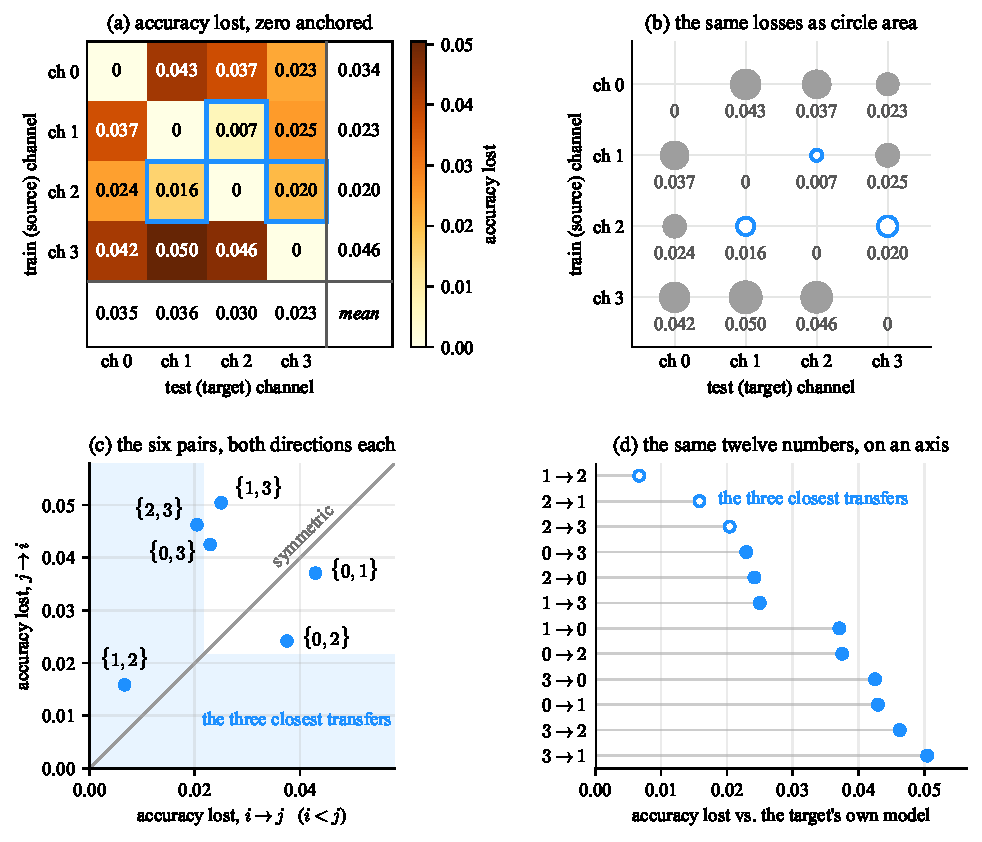
\includegraphics{plot_matrix}
	\caption{The same record as the loss $\Delta_{ij}$ of Eq.~\eqref{eq-plot-matrix-gap}, read four ways. (a) The loss anchored at zero, the row and column means in the margin band. (b) The same layout with the fill replaced by a mark whose area carries the loss and the value printed under it; the three closest transfers are the open rings, and the largest loss is $7.6$ times the smallest, which is $7.6$ times the area of its mark and $2.7$ times its diameter. (c) One point per pair, its two directions its two coordinates, the lower-indexed source on the horizontal axis; the shaded band holds the three closest transfers, so a point inside it has a direction among them, and $\{1,2\}$, inside both arms, transfers well each way. (d) The same twelve losses on a common scale, sorted.}
	\label{fig-plot-matrix}
\end{figure}

Panel~(b) keeps the layout of (a) and changes the mark. The loss becomes the area of a circle, fourth in the ranking of Sec.~\ref{sec-app-plot-encoding} where shading is sixth, and three things follow from that alone. No cell is judged against the shade of its neighbors, which is what Sec.~\ref{sec-app-plot-context} says a filled grid cannot avoid. An exact zero draws nothing, so the diagonal empties itself rather than having to be blanked. And the panel needs no colorbar, because the value is printed under every mark, which is what a magnitude channel owes the reader in place of a key. What the area gives up is precision: the largest loss is $7.6$ times the smallest, so its mark has $7.6$ times the area and only $2.7$ times the diameter, which is the length the eye compares.

Panels~(c) and~(d) put the same twelve losses at the top of the ranking, as position on a common scale. Panel~(c) also answers what a grid invites and no reader performs, whether the relation is symmetric. It is not.

Circle area is not the only mark that frees a cell of its fill. Fig.~\ref{fig-plot-matrix-forms} keeps the layout and runs it through four of them. Only length can be ranked by eye.

\begin{box_yellow}[Every magnitude channel needs a zero and a key]
	Shading, area and stroke width are all magnitude channels, and each needs a zero the scale is anchored to, and a key on the page stating what one unit of the mark is worth.
\end{box_yellow}

\begin{figure}[ht]
	\centering
	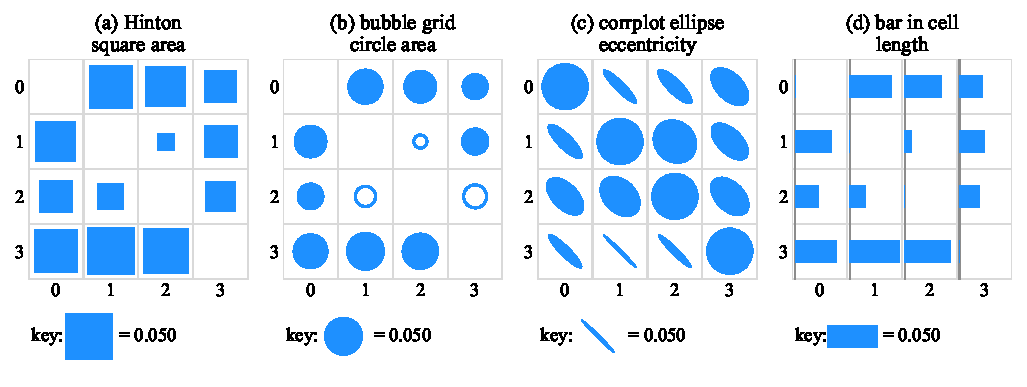
\includegraphics{plot_matrix_forms}
	\caption{One matrix of losses, four marks, one cell size, one key per panel. (a) The Hinton diagram, square area, and (b) the bubble grid, circle area, both 4\textsuperscript{th} in the ranking: an exact zero draws nothing, so the diagonal disappears without being told to, and (b) leaves color free for a second variable, here the three closest transfers. (c) The \texttt{corrplot} ellipse, eccentricity, third, built for a signed bounded quantity, so the largest mark of the panel lands on the diagonal. Difference between diagonal circiles is indistingushable. (d) The bar in cell, length from a common baseline, second, the only panel that can be ranked by eye. The extremes differ by a factor of $7.6$, which is $7.6$ times the area and $2.7$ times the side.}
	\label{fig-plot-matrix-forms}
\end{figure}
\FloatBarrier

\section{Axes}\label{sec-app-plot-axes}

The axis is where a plot is most often quietly wrong, because the same choice is legitimate for one encoding and misleading for another.

\subsection{The zero baseline}

Whether an axis must include zero is decided by the encoding, not by convention. A bar encodes its value as a \emph{length} measured from the baseline. A line encodes \emph{position}, so cutting the axis rescales the whole picture uniformly and the reader can see the axis labels. Fig.~\ref{fig-plot-baseline} is the bar case and Fig.~\ref{fig-plot-cutaxis} the position case.

\begin{figure}[ht]
	\centering
	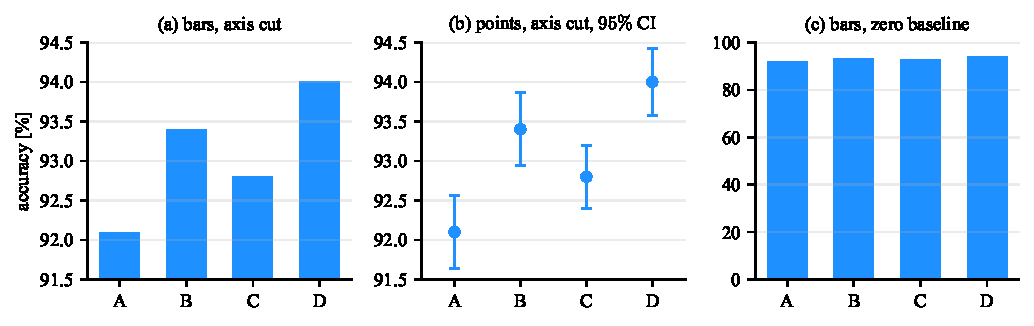
\includegraphics{plot_baseline}
	\caption{Four test accuracies, $92.1$, $93.4$, $92.8$ and $94.0$ percent. (a) With the axis cut at $91.5$, the bar for $D$ is $4.2$ times the length of the bar for $A$, though the values differ by $2\%$: an exaggeration of a factor of $4.1$. (b) The same numbers as points, on the same cut axis as (a), with the $95\%$ confidence interval of each over its $5$ folds. The cut is legitimate here and not in (a), because a point is at a position while a bar is a length measured from the baseline. The panel also reports what neither bar panel can: $B$ at $93.40 \pm 0.46$ and $D$ at $94.00 \pm 0.43$ are separated from $A$ at $92.10 \pm 0.46$, and $C$ at $92.80 \pm 0.40$ is not. (c) The same numbers as bars on a zero baseline, where the four models are correctly seen to be nearly tied.}
	\label{fig-plot-baseline}
\end{figure}

\begin{box_red}[A cut bar chart is not a style choice]
	Panel~(a) of Fig.~\ref{fig-plot-baseline} is the most common misleading chart in circulation, and it is usually produced by accident: many libraries auto-scale the axis to the data range, so cutting the baseline is what happens when nothing is specified. Any bar chart whose baseline is not zero should be treated as an error to be fixed, not a decision to be defended. 
	
	If the differences are too small to see on a zero baseline and they matter, plot the differences themselves, with their confidence intervals, on a zero that means \textit{no difference}.
\end{box_red}

The rule is about bars, and it does not run backwards: an axis that includes zero is not automatically the safer one. Fig.~\ref{fig-plot-cutaxis} is the same argument from the other side, on a quantity whose marks encode position.

\begin{figure}[ht]
	\centering
	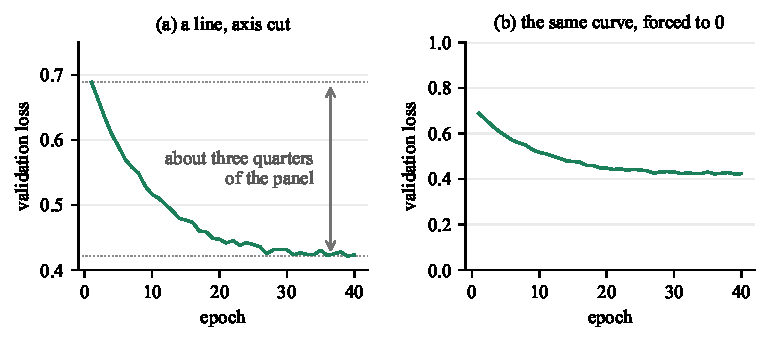
\includegraphics{plot_cutaxis}
	\caption{A $40$-epoch validation loss, drawn twice. (a) The marks encode position, the axis is labeled, the decay and the plateau are both readable, and the limits are chosen so that the curve fills the marked $76\%$ of the panel. (b) The identical curve forced onto $0$ to $1$.}
	\label{fig-plot-cutaxis}
\end{figure}

Forcing zero onto panel~(b) does not make it honest, it deletes the finding: the plateau is left with is less than the separation at which a reader resolves anything at all. Nothing is gained in exchange, because no mark in the panel is a length measured from the baseline, so there is no length for the cut to distort.

\begin{box_yellow}[How far to cut]
	A cut is a choice of limits, not just a decision to leave zero out. Choose them so that the data fill about two thirds to three quarters of the panel. 
\end{box_yellow}

\subsection{Cumulative totals}\label{sec-app-plot-cumulative}

The baseline is not the only way a chart can be exactly right about its numbers and wrong about the question. A running total is monotone by construction: it cannot fall, whatever the process underneath it does, so it always draws a rising curve. Presented as evidence that an effort is working, it is evidence of nothing. Fig.~\ref{fig-plot-cumulative} plots one record both ways.

\begin{figure}[ht]
	\centering
	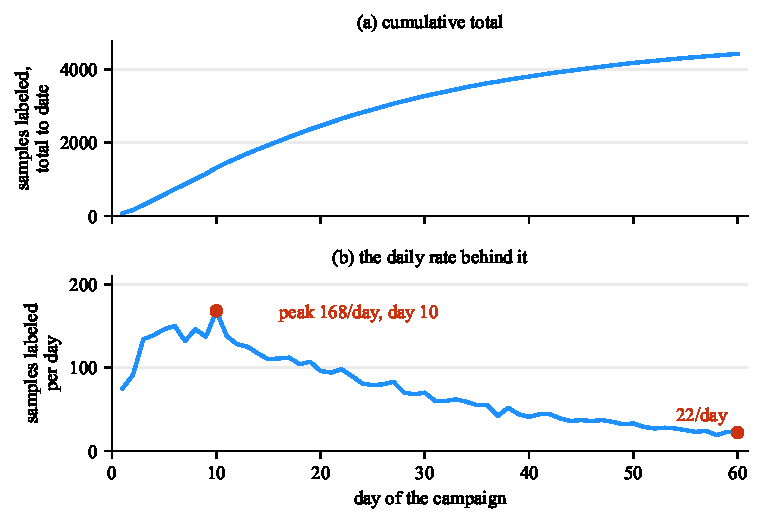
\includegraphics{plot_cumulative}
	\caption{A $60$-day labeling campaign, plotted as a total and as a rate. (a) The running total climbs to $4429$ samples and rises on every one of its $59$ steps, since a cumulative curve cannot do anything else. (b) The daily rate that produced it: a peak of $168$ per day on day $10$, falling to $22$ per day by day $60$, which is $13\%$ of the peak. The first week contributed $20\%$ of the total and the last week $4\%$. Both panels are exact, and only (b) answers whether the campaign is still working.}
	\label{fig-plot-cumulative}
\end{figure}

\begin{box_red}
Plot the quantity the question is about!
\end{box_red}

\FloatBarrier
\subsection{Aspect ratio}

The physical shape of the axes changes the slope a reader perceives, and slope is how a line chart is read. Fig.~\ref{fig-plot-aspect} draws one series five times with identical axis limits: the first three change the height of the axes, and the last two repeat the third of them at two thirds and at a third of its width.

\begin{figure}[ht]
	\centering
	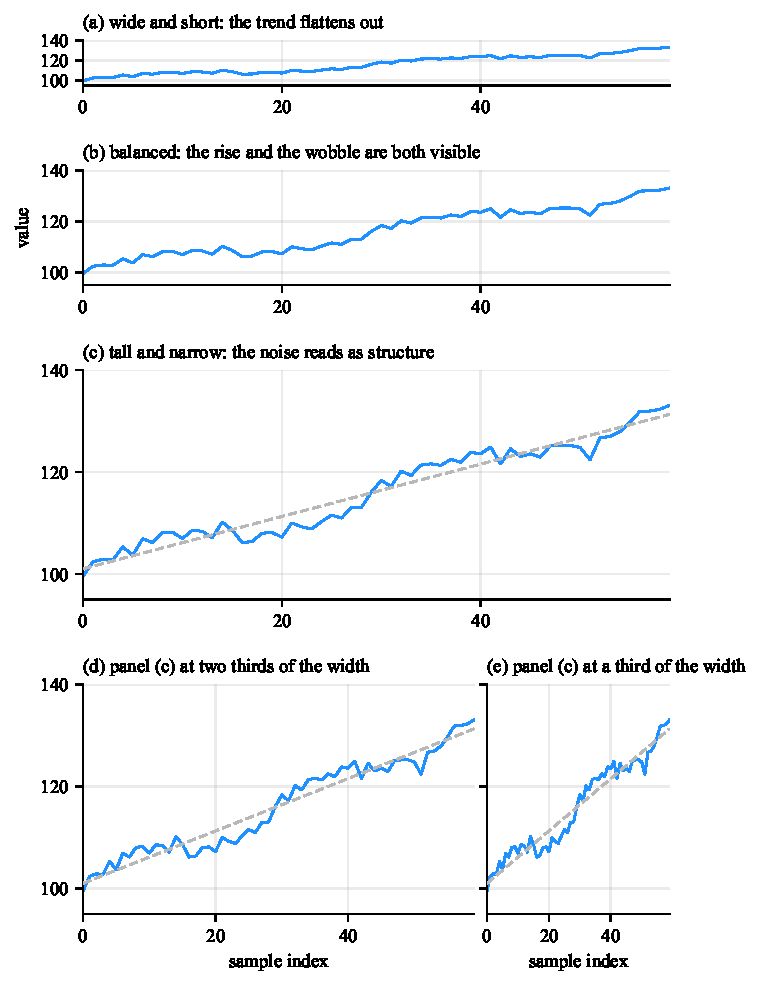
\includegraphics{plot_aspect}
	\caption{One series, one pair of axis limits, five axes shapes. The median segment of the line meets the horizontal at $7.0^{\circ}$ in (a), $17.5^{\circ}$ in (b) and $32.2^{\circ}$ in (c), so the slope the reader perceives grows with the height of the axes. Panels (d) and (e) are (c) narrowed to two thirds and to a third of its width, which delivers $43.4^{\circ}$ and $63.7^{\circ}$.}
	\label{fig-plot-aspect}
\end{figure}

\textit{Ad hoc} Cleveland's rule of thumb is to \emph{bank to $45^{\circ}$}: choose the aspect ratio so that the typical line segment meets the horizontal near $45^{\circ}$, since that is where a change in slope is easiest to detect. 

\FloatBarrier
\subsection{Ticks and labels}\label{sec-app-plot-ticks}
\begin{box_yellow}[Easy numbers]
Ticks at $1$, $2$, $5$, $10$ and their mulitplications/powers, never at the $7$ or $13$ an algorithm sometimes lands on.
\end{box_yellow}
\begin{box_yellow}[Labeled axes]
Every axis names a quantity and a unit. A number without a unit is not a measurement.
\end{box_yellow}
\begin{box_yellow}[Compress offset]
 A quantity far from zero has its level stated on the panel and its deviation ticked in a unit sized to the drift. An offset parked in a corner box, or spelled out on every tick, both leave the reader doing arithmetic.
\end{box_yellow}
Fig.~\ref{fig-plot-ticks}(a) does what a reader normally asks for and puts the full value on every tick, and this record will not support it: six digits a label to report a drift of $131$~mK, so the level is printed five times over, the quantity the figure is about is carried by the last two digits, and the ticks fall at $7$~s. 
State the level on the panel, and tick the deviation from it in a unit sized to the drift, which is panel~(b).
\begin{figure}[ht]
	\centering
	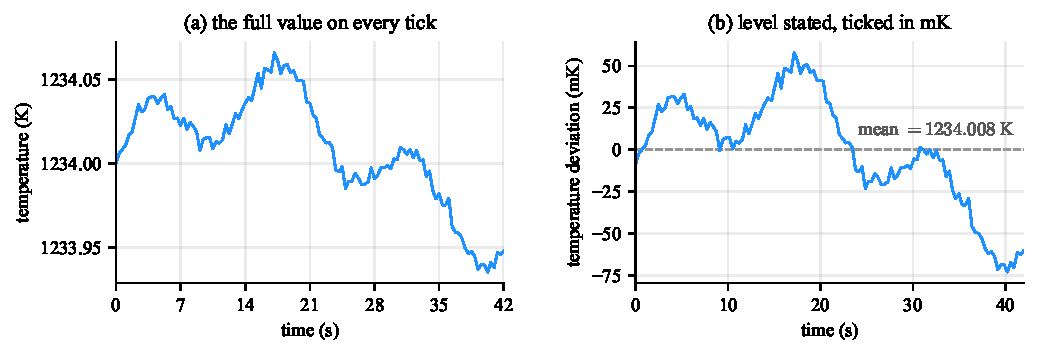
\includegraphics{plot_ticks}
	\caption{(a) The full value on every tick: the axis runs $1233.90$ to $1234.10$~K in steps of $0.05$~K, which is six digits a label of which only the last two carry the drift, and the ticks fall at $7$~s. (b) The same record with the level subtracted and the deviation from it ticked in millikelvin: ticks at $10$~s and $25$~mK, every one of them a small round number. Zero on this axis is the mean and nothing else, the dashed line marks it and names it in full, $1234.008$~K, so any mark on the panel converts back to an absolute temperature, and the record is seen to run $-73$ to $+58$~mK about it.}
	\label{fig-plot-ticks}
\end{figure}

\begin{box_yellow}
 And treat rotated tick labels as a diagnostic rather than a solution: if the label names do not fit horizontally, the chart wants to be horizontal.
\end{box_yellow}
Rotating a label is not a style preference (Fig.~\ref{fig-plot-rotated}). 
The six names are the same in both panels and so are the six numbers; what changes is where the names are kept. Tilted under the axis they claim $18.3$~mm of a $66$~mm figure, which is $28\%$ of its height taken out of the bars, and the reader still has to read them at an angle. Turned on their side they claim $22.8$~mm of width, which comes out of the margin rather than the panel, and the same figure gives the bars $47.2$~mm of height instead of $37.6$.

\begin{figure}[ht]
	\centering
	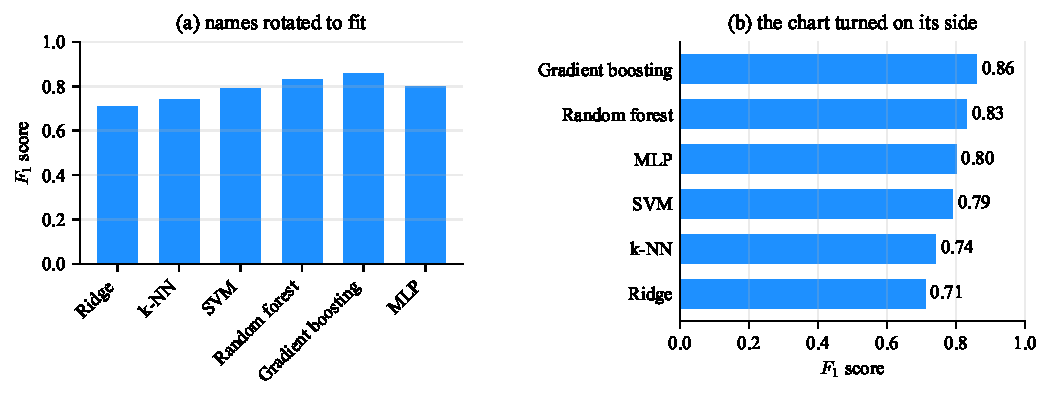
\includegraphics{plot_rotated}
	\caption{Six $F_1$ scores drawn twice in one figure box with nothing changed but where the category names are kept. (a) Names tilted at $45^{\circ}$ to fit under a vertical axis. (b) The chart turned on its side.}
	\label{fig-plot-rotated}
\end{figure}

\subsection{Legends}\label{sec-app-plot-legend}

A series has to be named somewhere, and there are only two approaches to put the name; the two differ in which of the two reading operations of Sec.~\ref{sec-app-plot-lookup} the reader is made to perform.

\begin{itemize}
	\item A \emph{boxed legend} is a key set apart from the data, mapping a color or a line style to a name. Reading it is a table look-up, and it is a look-up per mark: the reader carries a color/style to the box, finds the matching key, carries the name back, and repeats it for the next series.
	\item An \emph{end-of-line label} is the name set at the end of the series it belongs to, in that series' color. There is nothing to carry anywhere, because the name is already where the reader is looking.
\end{itemize}

Fig.~\ref{fig-plot-legend} draws four curves both ways.

\begin{figure}[ht]
	\centering
	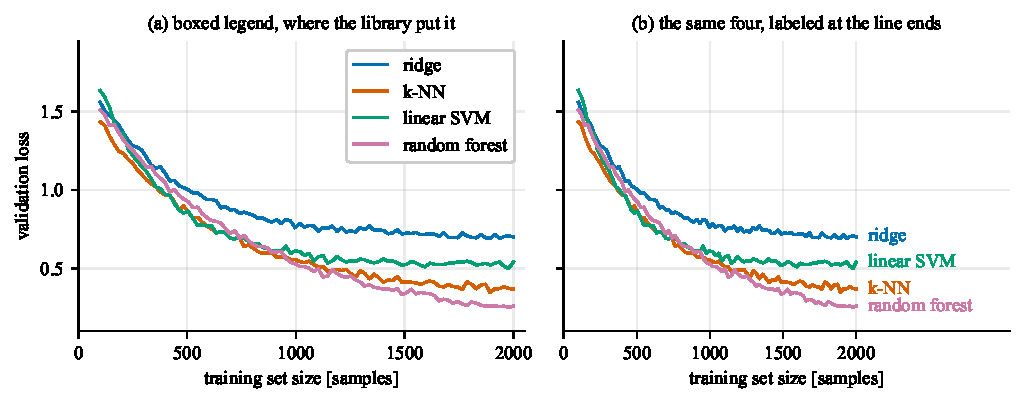
\includegraphics{plot_legend}
	\caption{Learning curves for four models on identical axes, named two ways. (a) A boxed legend at the position the library chose: it spends $15\%$ of the panel on the key, and its entries are in the order the series were plotted, which is not the order they arrive in at the right edge, so $2$ of the $4$ are out of place and the reader re-sorts on every look-up. (b) The same four named where they end. No panel area is spent, no color has to be carried anywhere, and the names survive a gray print and a color vision deficiency simulation because there the name identifies the curve and the color only decorates it.}
	\label{fig-plot-legend}
\end{figure}

Three consequences, in the order they usually matter.

\emph{Label directly whenever there is room.} It removes the look-up entirely.

\emph{Where a box is unavoidable, order it to match the page.} Sort its entries to match the vertical order of the series at the edge where the reader meets them, and place it over a region carrying no data. 

\emph{What the key is made of decides what the look-up costs.} A key is read no faster than the channel it maps. Dash patterns and marker shapes are \textit{nominal}: the entries have no order among them, so each is matched glyph by glyph, and the match is made again wherever the curves cross, which is exactly where the glyphs are hardest to tell apart. Line width and lightness are \textit{ordered}: moved together they turn the key into a sequence, read once and then predicted, and its entries come out in the order the curves appear on the page, which is the previous rule obtained for nothing. Fig.~\ref{fig-plot-patterned} is one record under both.

\begin{figure}[ht]
	\centering
	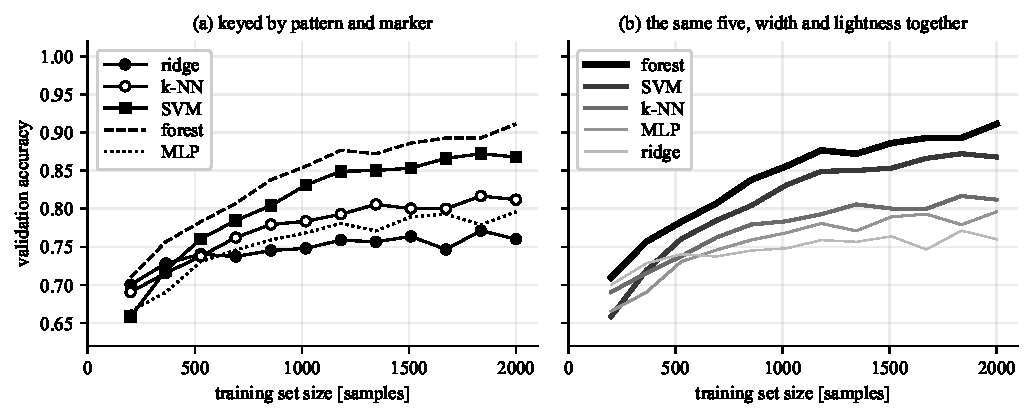
\includegraphics{plot_patterned}
	\caption{Five plot with a boxed legend in both panels. (a) Keyed by dash pattern and marker shape. The five entries have no order among them. (b) The same five keyed by one ladder, line width from $2.6$ to $0.7$~pt and gray from $0.00$ to $0.72$.}
	\label{fig-plot-patterned}
\end{figure}

\begin{box_blue}[The one place redundancy is worth its ink]
	Encoding a quantity twice is normally waste (Sec.~\ref{sec-app-plot-dataink}), and panel~(b) does it on purpose: the rank of a series is in its width and in its lightness at once. 
\end{box_blue}

\emph{With $6+$ series, neither form works.} End labels start to collide wherever the series converge, a box with a dozen keys is a second figure to read before the first one can be, and no ladder has a dozen separable steps either. That is the point at which the answer is small multiples (Sec.~\ref{sec-app-plot-many}) or highlighting one series against gray (Fig.~\ref{fig-plot-highlight}), not a smaller font.

\FloatBarrier

\subsection{Many plots at once}\label{sec-app-plot-many}
\begin{goal}
	What does a reader do with ten series that will not fit on one axis?
\end{goal}
Legend won't help.
Stop drawing one plot and draw many: one panel per series, laid out as a grid, every panel on the same range. The grid is called \emph{small multiples}. Fig.~\ref{fig-plot-small-multiples} is the overlay beside its replacement.

\begin{figure}[ht]
	\centering
	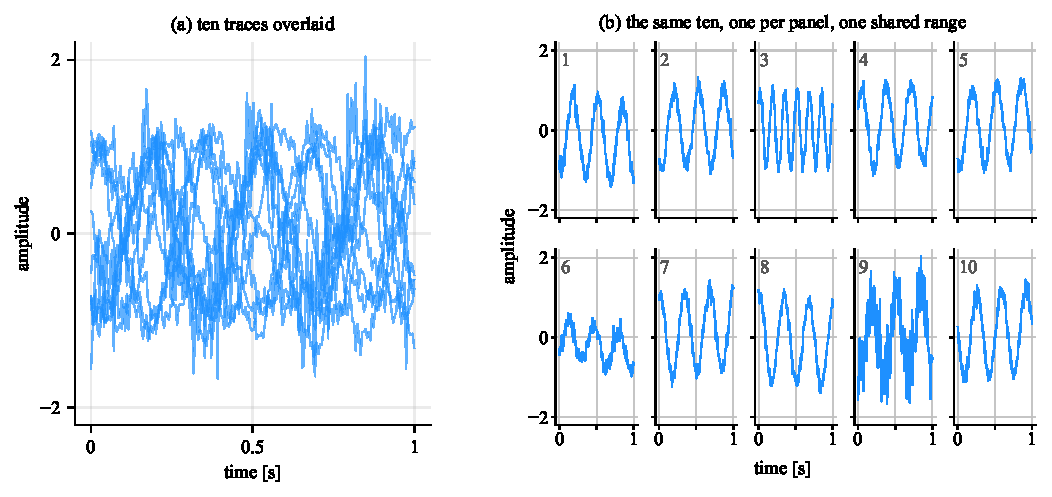
\includegraphics{plot_small_multiples}
	\caption{Ten recordings from one process. (a) Overlaid: the envelope is readable and nothing else is. (b) The same ten as \emph{small multiples}, one panel each, on one linked range. Three of the ten are not like the rest, in three different ways: trace $3$ runs at $6$~Hz against the $3$~Hz of the others, trace $6$ has $0.55$ of their amplitude, and trace $9$ carries $4.1$ times their noise. Not one of the three can be found in (a).}
	\label{fig-plot-small-multiples}
\end{figure}

\begin{itemize}
	\item \emph{One range, set once.} Give the panels a single range on both axes and link them, so that the range is a property of the block rather than ten separate decisions. Per-panel autoscaling is the default in most libraries, and it produces ten plots that look like a comparison and \textit{are not} one.
	\item \emph{Values on the outer edge only.} The left column carries the $y$ values and the bottom row the $x$ values, and one label of each names the block. Ten copies of one axis is nine copies of ink, which is Sec.~\ref{sec-app-plot-dataink} applied to a layout.
	\item \emph{Rule every panel, at the ticks it keeps.} A panel stripped of its scale reports a shape and no quantity, exactly as a close-up does (Sec.~\ref{sec-app-plot-closeup}), and the separation still has to clear the limit of Sec.~\ref{sec-app-plot-gridlines} at the panel's reduced size.
\end{itemize}

\begin{box_blue}
	Sec.~\ref{sec-app-plot-perception} to answer ``where is this one among the rest'' at a glance, and can be repeated across a row of panels to walk through several. Fig.~\ref{fig-plot-highlight} is the comparison, on twelve series that an overlay cannot separate.
\end{box_blue}

\FloatBarrier
\subsection{Close-ups}\label{sec-app-plot-closeup}

One axis range cannot always serve both the extent of a record and a feature inside it. A transient a few milliseconds wide, drawn across a panel that covers seconds, gets a fraction of a millimeter of the page whatever the aspect ratio, and no amount of care with the ticks recovers it. The answer is a second view at a second scale, and it comes in two forms.

\begin{itemize}
	\item An \emph{inset}: a small second axes drawn inside the panel, in a region that carries no data. It keeps the overview and the detail in one frame, and it costs nothing but the space it occupies.
	\item A \emph{broken-out panel}: the same window as a full panel beside the overview. It is the answer when the parent has no free corner, when the zoom needs its own axis labels, or when the required magnification is large enough that a small inset would not resolve the feature anyway.
\end{itemize}

Fig.~\ref{fig-plot-closeup} draws one record all three ways.

\begin{figure}[ht]
	\centering
	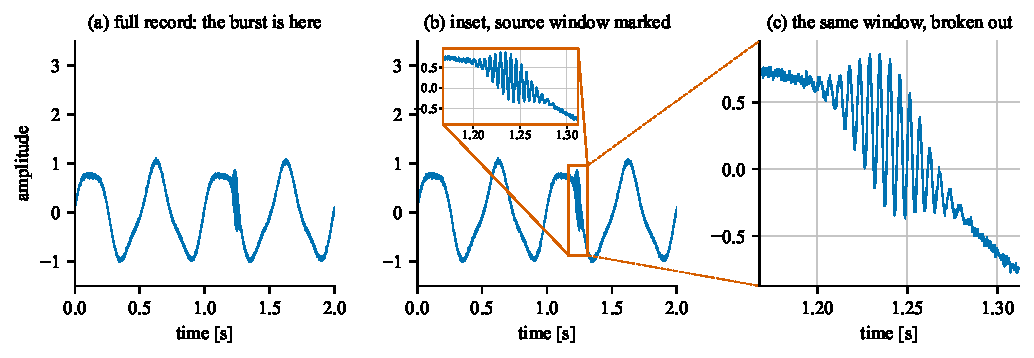
\includegraphics{plot_closeup}
	\caption{A $2$~s record sampled at $5$~kHz, carrying a $180$~Hz burst on a $2$~Hz carrier, a frequency ratio of $90$. (a) The full record: the burst is at $1.24$~s, it is the only thing the record is about. (b) An inset over the $144$~ms window that contains it, a magnification of $14$, with the source window boxed on the parent and connected to the inset so the reader can locate what was magnified. (c) The same samples as a panel of their own, which is what the window needs when the parent has no room.}
	\label{fig-plot-closeup}
\end{figure}

\begin{itemize}
	\item \emph{Mark the source window} with a rectangle on the parent panel, and connect the rectangle to the view it produced. 
	\item \emph{Keep the ticks on the close-up, and rule it at them.} A zoom without a scale shows a shape and reports no quantity, and the reader has no way to tell a $10$-fold magnification from a $100$-fold one. Ticks are the minimum; the grid at those ticks is what turns the magnified shape into values the reader can take off the page (Sec.~\ref{sec-app-plot-gridlines}), and a close-up is read for values rather than for where the feature sits.
	\item \emph{Put the inset where there is no data.} If the panel has no empty region, that is the signal to break the view out into its own panel rather than to cover the trace with it.
\end{itemize}
\FloatBarrier

\subsection{Size and gridlines}\label{sec-app-plot-gridlines}
\begin{goal}
	How tall must a panel be, and how finely may it be ruled?
\end{goal}
\begin{box_yellow}[Two rules for the grid]
\begin{itemize}
	\item Rule the panel. The grid is the route from a mark to a number, and adding one improved accuracy at every size measured.
	\item Do not shrink a panel below the height at which its scale can be read.
	\item Do not rule it more finely than the reader can resolve. 
	\item At a typical rendering of $96$ pixels per inch that is a height of about $2$~cm and a gridline separation of at least $2$~mm, both measured on the printed page rather than on the screen the figure was authored on.
\end{itemize}	
\end{box_yellow}

Both numbers are measured rather than chosen, and two results are what the measurement leaves for use.\footnote{Heer and Bostock, \href{https://doi.org/10.1145/1753326.1753357}{``Crowdsourcing Graphical Perception''} (CHI, 2010), third experiment.} 
\begin{itemize}
	\item On a $0$ to $100$ scale, gridlines every $10$ or $20$ units beat gridlines every $50$ or $100$.
	\item Not usefull once the lines fall closer together than the reader can separate them, which is about $8$ pixels, or $2$~mm at final size.
\end{itemize}

The default is often no grid at all, or a line every $50$ units, and both leave the reader interpolating a value across half the panel. Fig.~\ref{fig-plot-gridsize} is that case beside its fix, at one panel size, so the ruling is the only thing that changes between the two. 

\begin{figure}[ht]
	\centering
	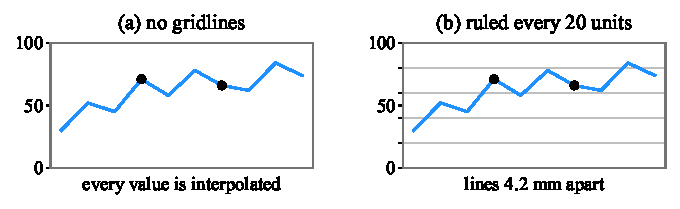
\includegraphics{plot_gridsize}
	\caption{One series on a $0$ to $100$ scale, with the two values a reader is asked to compare, $71$ and $66$, marked. Both panels are $80$ pixels tall, that is $21.2$~mm at $96$ pixels per inch, and they differ in nothing but the ruling. (a) No gridlines by default. (b) The same panel ruled every $20$ units, which is $4.2$~mm at this height and twice the $2.1$~mm the eye needs to keep two lines apart: each marked value now sits against a line instead of being estimated.}
	\label{fig-plot-gridsize}
\end{figure}


\FloatBarrier
\subsection{Logarithmic Axes}\label{sec-app-plot-logscale}

When a quantity spans several orders of magnitude, a linear axis shows the largest decade and compresses everything else onto the baseline (Fig.~\ref{fig-plot-logscale}). 

\begin{figure}[ht]
	\centering
	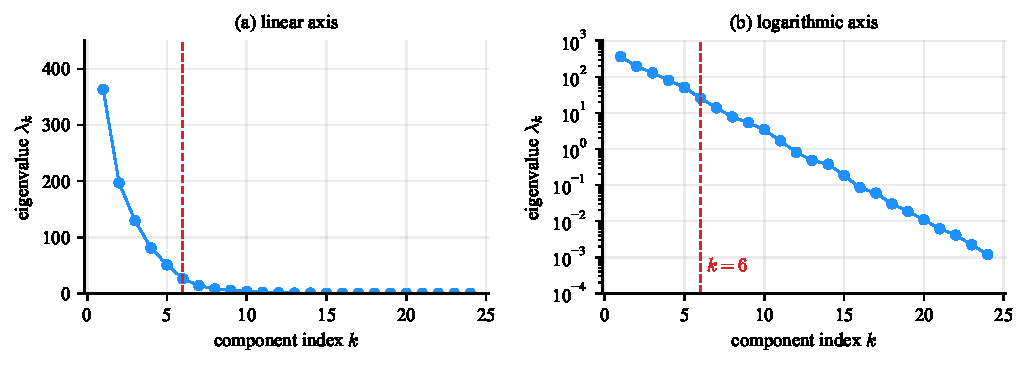
\includegraphics{plot_logscale}
	\caption{An eigenvalue spectrum spanning five and a half decades, from $363$ to $0.0012$. (a) On a linear axis, $15$ of the $24$ eigenvalues fall below $1\%$ of the largest and are pinned to the baseline, indistinguishable from one another and from zero. (b) On a logarithmic axis, the same spectrum is a straight line, which identifies the decay as exponential, and the change of regime at the dashed line becomes something the reader can locate rather than guess.}
	\label{fig-plot-logscale}
\end{figure}

\begin{box_yellow}[No zero or negative values]
	A log axis cannot show zero or negative values, so a curve that reaches zero needs a different treatment
\end{box_yellow}
\FloatBarrier

\section{Choosing a Font}\label{sec-app-plot-fonts}

\begin{box_yellow}
A figure's text is document text. It is read on the same page, at the same distance, as the body around it.
\begin{itemize}
	\item Text sized at the width the figure will actually be printed at.
	\item One font (at least family) throughout the figure, text and math.
\end{itemize}
\end{box_yellow}

\subsection{Figure size sets the text size}
Point size is fixed in the script while the figure is scaled to fit the page, so the two are tied by one relation. A figure authored at width $w_a$ and placed at width $w_p$ has every glyph scaled by $s = w_p / w_a$, and the size the reader actually gets is
\begin{equation}
	p_{\mathrm{page}} = s\,p_{\mathrm{script}}.
	\label{eq-plot-fontscale}
\end{equation}
Authored at $15$~cm and placed at $8.8$~cm gives $s = 0.59$, so a $10$~pt tick label arrives at $5.9$~pt. Nothing in the script announces this, and nothing in the figure looks wrong until it is printed.

The reliable fix is $s = 1$: set the figure width to the width it will occupy and place it without a \texttt{width=} override, so a point in the script is a point on the page. Fig.~\ref{fig-plot-fonts} is drawn that way, which is what lets each of its panels be read twice over.

\begin{figure}[ht]
	\centering
	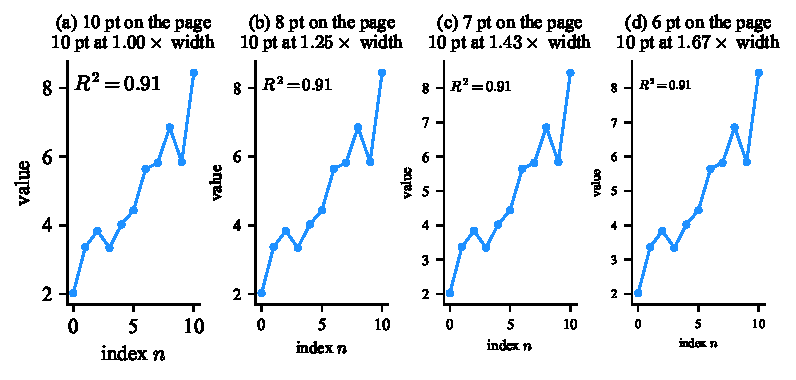
\includegraphics{plot_fonts}
	\caption{Type in a figure, at the size it is printed at. (a) to (d) One panel drawn four times, its labels at $10$, $8$, $7$ and $6$~pt. Each panel is also the second reading of its own subtitle: $6$~pt on the page is what a $10$~pt setting delivers once the figure has been authored at $1.67$ times its final width.}
	\label{fig-plot-fonts}
\end{figure}

\subsection{The three kinds of face}

Three distinctions cover what a plotting library will offer, and only the last of them is a matter of mechanism rather than appearance.

\begin{itemize}
	\item \emph{Serif}: small terminal strokes on the letters, the feet and heads magnified in Fig.~\ref{fig-plot-serif}. It matches most printed body text, which makes it the default for a figure that will sit inside a document.
	\item \emph{Sans-serif}: no terminal strokes, and a more even stroke weight. It survives small size, low resolution and a poor projector better, for the direct reason that the first detail to disappear in a serif face is the serif.
	\item \emph{Monospace}: every character claims the same width, so an \texttt{i} occupies as much room as an \texttt{m}. That is the entire difference, and Fig.~\ref{fig-plot-faces} is it: eight \texttt{i} and eight \texttt{m} end at the same place in the monospace column and nowhere else.
\end{itemize}

The first two of the three differ in one detail, and it is a small one. At the size a label is actually read, a serif is a fraction of a millimeter of ink at the end of a stroke, which is why it takes a magnification to see what is being talked about, and why it is the first thing lost when the figure is shrunk or projected.

\begin{figure}[ht]
	\centering
	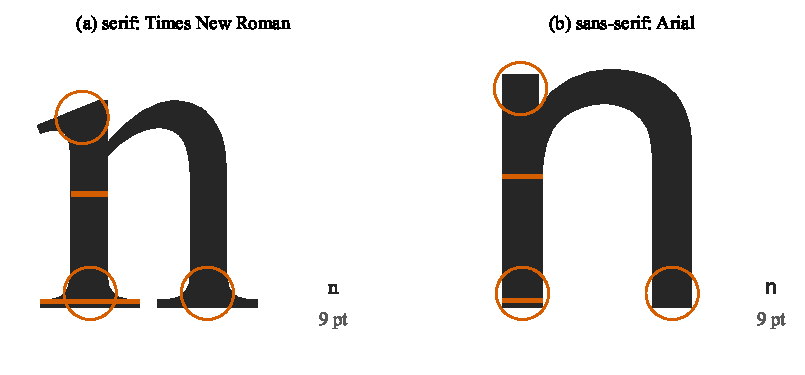
\includegraphics{plot_serif}
	\caption{The letter \texttt{n} at $200$~pt, a magnification of $22$ over the $9$~pt it is read at, drawn in the two text faces at one scale, with the same letter at reading size beside it. The bars measure the left stem where it is a stem and where it meets the baseline: in Times New Roman the foot is $2.8$ times the stem, and in Arial the foot is the stem, $1.00$. The rings mark the head of that stem and both feet of the letter, each placed where the ink was found rather than by hand; in (b) they enclose plain cut ends.}
	\label{fig-plot-serif}
\end{figure}

\begin{figure}[ht]
	\centering
	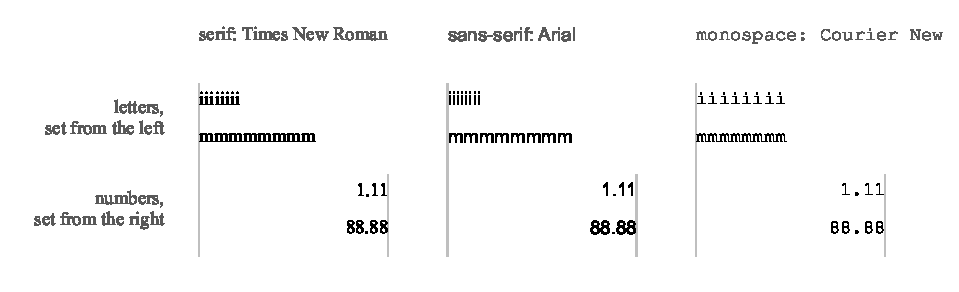
\includegraphics{plot_faces}
	\caption{The same eight letters and the same two numbers in the three kinds of face, set against a left guide and a right guide. The $\texttt{i}$ and $\texttt{m}$ rows end together only in the monospace column, where both letters claim $6.00$~pt; in the other two an $\texttt{i}$ claims $0.36$ and $0.27$ of an $\texttt{m}$. The number rows align in all three, because digits are drawn to one width in text faces as well.}
	\label{fig-plot-faces}
\end{figure}

Monospace is worth reaching for when the text is something that was literally typed, since it preserves indentation and lets a reader count characters: code, file names, hex color codes such as the \texttt{\#1F77B4} of Sec.~\ref{sec-app-plot-colorspace}.

\begin{box_blue}[Monospace is for programers]
Monospace is commonly used for programing environments. Modern font families features a "texture healing" technique that softens the wide gaps usually found in fixed-width text, improving code readability while keeping a strict vertical grid. 
\end{box_blue}

Between serif and sans there is no reliable difference in reading speed to appeal to. That choice is settled by the medium and by the document the figure will sit in, not by preference.

That is a statement about reading speed, and it is not a statement about everything else. Fig.~\ref{fig-plot-baskerville} is the case that makes the difference.

\begin{figure}[ht]
	\centering
	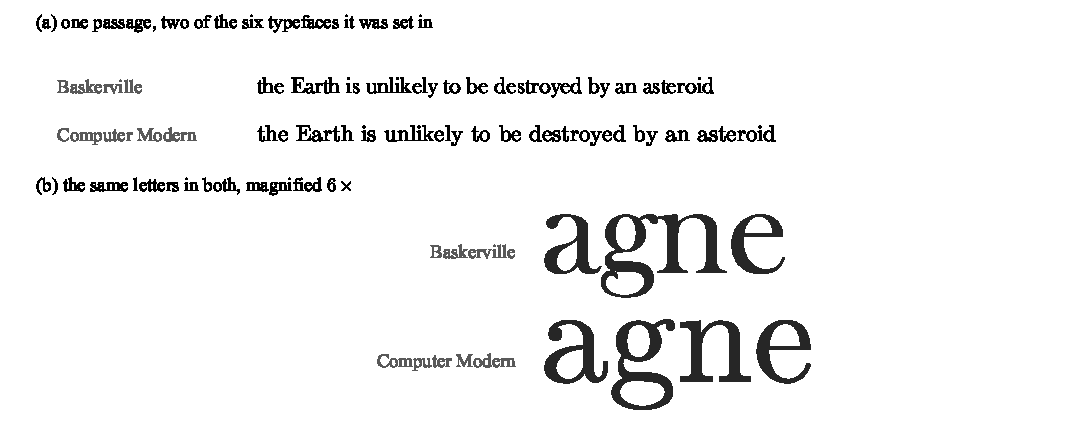
\includegraphics{plot_baskerville}
	\caption{Two of the six typefaces of the experiment described below, the one that came first and the one that came second. (a) The same passage in both, at $11$~pt, which is how the readers met it. (b) The same four letters magnified $6$ times. The two faces differ far below the $2$~mm at which detail stops being resolved.}
	\label{fig-plot-baskerville}
\end{figure}

\begin{box_blue}[Two faces that look alike, and did not perform alike]
	In 2012 a newspaper ran a quiz that was really a typography experiment.\footnote{Errol Morris, \href{https://archive.nytimes.com/opinionator.blogs.nytimes.com/2012/08/08/hear-all-ye-people-hearken-o-earth/}{``Hear, All Ye People; Hearken, O Earth''}, \emph{The New York Times}, 2012, with the analysis by David Dunning and Benjamin Berman.} Readers were shown one passage, arguing that the Earth is unlikely to be destroyed by an asteroid, and asked whether they agreed with it. What varied was the typeface: each reader was assigned one of six at random, among them Baskerville, Computer Modern, Georgia, Helvetica and Comic Sans. About $45\,000$ answers came back.

	Agreement ran about $1.5$ percentage points higher in Baskerville than in the rest, significant at $p < 0.01$ on that sample. Computer Modern was the runner-up and Comic Sans came last. The two at the top are the pair in Fig.~\ref{fig-plot-baskerville}, and that is the finding worth carrying: they are two serif book faces that an ordinary reader cannot name, cannot tell apart in running text, and was not asked about. Whatever produced the difference, it was not anybody noticing the typeface.

	What may not be concluded is that a typeface can be chosen for trust. It is one experiment, on one passage, with an effect of a percentage point and a half: large enough to measure at that sample size, and far too small to design around. What it does establish is that the face is never neutral, which is a reason to set it deliberately rather than to inherit it from the library.
\end{box_blue}

\section{How a Reader Groups Marks}\label{sec-app-plot-gestalt}
A reader does not perceive marks individually and then assemble them. Grouping happens first, automatically, and follows a set of regularities. Three of them do most of the work inside ordinary charts, and Fig.~\ref{fig-plot-gestalt} shows each doing it.

\begin{figure}[ht]
	\centering
	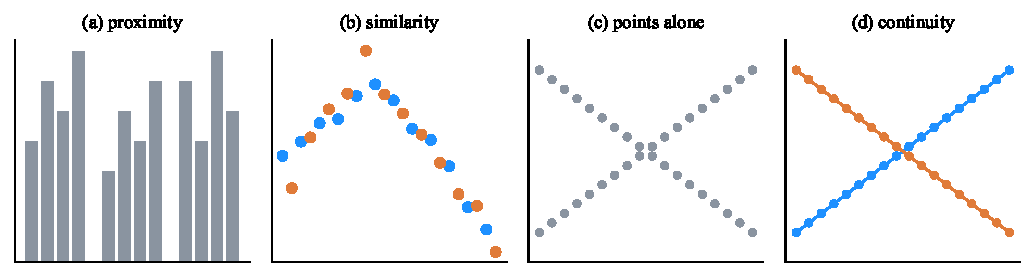
\includegraphics{plot_gestalt}
	\caption{Grouping laws inside charts. (a) Proximity: twelve bars at uniform height spacing read as three groups of four, purely from the gaps. (b) Similarity: one set of points in two colors reads as two interleaved series. (c) and (d) Continuity: identical coordinates, drawn as loose points and then connected. Only the connected version resolves into two crossing curves.}
	\label{fig-plot-gestalt}
\end{figure}

Each law is a tool and a hazard, because it applies whether or not the grouping it produces is real.

\begin{itemize}
	\item \emph{Proximity} groups by spacing. Deliberate use: widen the gap between categories that belong to different conditions, and the reader sees the conditions without a legend. Accidental use: uneven spacing produced by a default layout invents groups that are not in the data.
	\item \emph{Similarity} groups by shared appearance. This is what makes a color legend work at all. It also means that two unrelated series drawn in similar colors will be read as one, and that reusing a color across panels asserts that the two things are the same thing.
	\item \emph{Continuity} is asserted by a connecting line, and a line is a claim that the samples between the marks lie on the path drawn. That claim is true for a time series and false for measurements at unordered categories. Connecting points across a gap in the recording makes the same false claim; break the line at the gap instead.
	\item \emph{Closure} lets a reader complete a shape from part of its outline, which is why a chart needs no box around it and no axis line on the side that carries no scale.
\end{itemize}

Similarity is more than alike or not alike. Where the series being grouped have an order of their own, the appearance that groups them can carry that order as well, as illustrated in Fig.~\ref{fig-plot-gradation}.

\begin{figure}[ht]
	\centering
	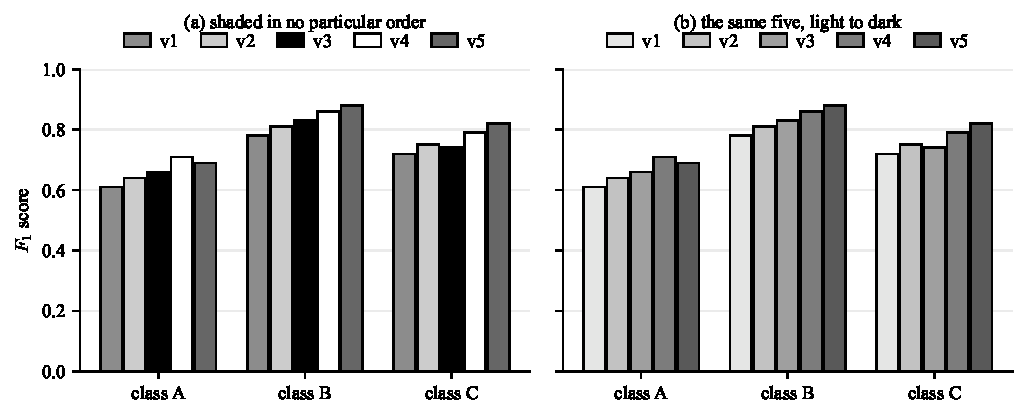
\includegraphics{plot_gradation}
	\caption{Five successive model versions scored on three classes, shaded two ways. Proximity makes the three groups in both panels, so what differs is whether a version can be traced from one group to the next. (a) Gray levels $0.55$, $0.80$, $0.00$, $1.00$ and $0.40$, taken in the order the versions come in. (b) The same numbers on a ramp from $0.90$ to $0.35$ in equal steps.}
	\label{fig-plot-gradation}
\end{figure}

\begin{box_yellow}[Shading a set of series]
	\begin{itemize}
	\item If the series have an order, encode it: one ramp, monotone in lightness, and let dark stand for one end of it throughout the figure. 
	\item If they have no order, use a qualitative scheme and do not imply one. 
	\end{itemize}
	Either way the reader is meant to get the grouping and the ranking from the same channel, without consulting the key twice.
\end{box_yellow}


\section{Transparency}\label{sec-app-plot-alpha}

Marks land on marks. In a dense scatter at full opacity the mark drawn last covers the ones drawn before it, so the panel reports the outline of the cloud and the accident of the draw order rather than what is inside it. Every library offers an opacity setting for exactly this problem: \texttt{alpha} in \texttt{matplotlib}, \texttt{FaceAlpha} and \texttt{EdgeAlpha} in MATLAB. A mark of color $c$ drawn at opacity $\alpha$ does not replace background color $c_{\mathrm{bg}}$ that lies under it, it is mixed into it,
\begin{equation}
	c_{\mathrm{out}} = \alpha\,c + (1-\alpha)\,c_{\mathrm{bg}} ,
	\label{eq-plot-alpha-over}
\end{equation}
so a second mark on the same spot mixes into the result of the first, a third into the result of the second, and after $n$ of them the ink accumulated is
\begin{equation}
	a_n = 1 - (1-\alpha)^n .
	\label{eq-plot-alpha-stack}
\end{equation}
Two consequences follow from the same two lines, and they are the two halves of this section. Darkness now reports how many marks are there, which is what makes transparency work at all, and darkness now reports how many marks are there whether or not that is what the figure meant to say.

\subsection{Misuse}\label{sec-app-plot-alpha-misuse}

Both failures in Fig.~\ref{fig-plot-alpha-misuse} come from the same place: an opacity was set for the appearance of a single mark, and Eq.~\eqref{eq-plot-alpha-over} was then applied to the places where the marks meet. Both fixes are the panel beside the failure, and they are the same fix: give the distinction to a channel that does not composite.

\begin{figure}[ht]
	\centering
	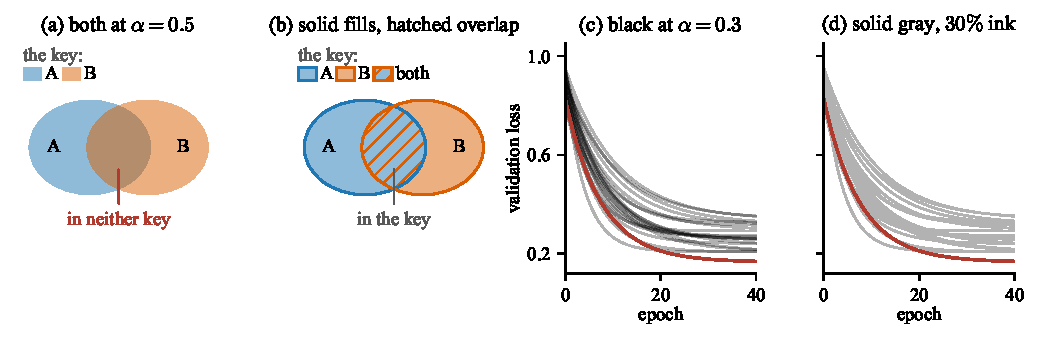
\includegraphics{plot_alpha_misuse}
	\caption{Two ways an opacity setting says something the figure did not intend. (a) Two class regions at $\alpha = 0.5$. The intersection renders as a third color that is in neither of them. (b) The same two regions with no opacity anywhere: both classes filled solid and outlined in their own key color, and the area they share carrying one fill under the other class color as a hatch, bounded by one arc of each outline. The page holds only the two colors the key names, the key names the shared area as well, and the draw order changes nothing. (c) and (d) Twenty runs behind the one under discussion: black at $\alpha = 0.3$ composites over white to exactly the $30\%$ ink gray of (d), so a lone curve is identical in the two panels and every difference between them is a crossing. Where the runs converge, up to $7$ of them fall within one line width, and that patch carries $92\%$ ink in (c) against the $30\%$ of a lone curve, a factor of $3.1$.}
	\label{fig-plot-alpha-misuse}
\end{figure}

\emph{Two categorical colors must never overlap at $\alpha$.} Fig.~\ref{fig-plot-alpha-misuse}(a) is the failure: the intersection of a blue region and an orange one is a third color, present in the figure and in neither key, and by Eq.~\eqref{eq-plot-alpha-over} which of the two possible mixtures it is depends on the order the two were drawn in. The legend is no help.
The remedy is to keep the classes in channels that cannot mix. Fig.~\ref{fig-plot-alpha-misuse}(b) fills both classes solid, outlines each in its own key color so the shared area has a boundary of its own, and hatches that area in the other class color: both class colors reach the page exactly as the key shows them, the shared area is visible without being a third color, and it is a third entry in the key rather than something the reader has to decode. Separate panels, or a single hue where the darkness means only ``more'', do the same job.

\begin{box_yellow}[Transparency changes the color]
	By Eq.~\eqref{eq-plot-alpha-over} the color on the page is not the color in the palette, and it changes again if the panel is later given a background: the same mark at $\alpha = 0.5$ is one color over white and another over a gray panel. So the gray print and the color vision deficiency checks of Sec.~\ref{sec-app-plot-checks} have to be run on the rendered figure rather than on the palette it was specified from, and a colormap loses its perceptual uniformity as soon as an opacity is applied to it.
\end{box_yellow}

\emph{For de-emphasis, use a light solid color rather than $\alpha$.} Drawing the context series in black at low opacity, is not the same as drawing them light: the crossings accumulate by Eq.~\eqref{eq-plot-alpha-stack} and darken wherever the series happen to bunch. Fig.~\ref{fig-plot-alpha-misuse}(c) and (d) are the same twenty runs de-emphasized both ways, matched so that a lone curve renders identically in the two panels. The alpha panel grows a dark bar exactly where the runs converge, which competes with the highlighted curve for the attention the highlight was supposed to own, and which reports a bunching that no key on the page quantifies.

\subsection{Accumulation}\label{sec-app-plot-alpha-accum}

Used deliberately, the same accumulation is the point: a dense scatter stops being a silhouette and becomes a density display. That makes $\alpha$ a magnitude channel, sixth in the ranking of Sec.~\ref{sec-app-plot-encoding}. It is also a channel that runs out, as Fig.~\ref{fig-plot-alpha-accum} shows.

\begin{figure}[ht]
	\centering
	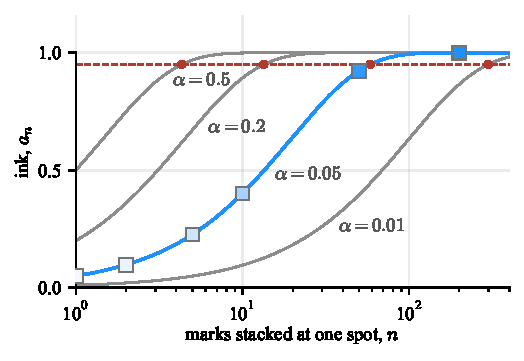
\includegraphics{plot_alpha_accum}
	\caption{The ink $a_n$ of Eq.~\eqref{eq-plot-alpha-stack} against the number of marks stacked at one spot, for four opacities. The squares on the $\alpha = 0.05$ curve are filled with the color the page actually renders at $n = 1$, $2$, $5$, $10$, $50$ and $200$, so the curve can be checked against its own ink. Past the dashed level at $0.95$, marked on each curve by a dot, a further mark changes nothing the reader can see.}
	\label{fig-plot-alpha-accum}
\end{figure}

\emph{Set $\alpha$ from the overlap, not by taste.} Eq.~\eqref{eq-plot-alpha-stack} saturates, and quickly. Ink reaches $95\%$ of full at $n^{\ast} = \ln(0.05) / \ln(1-\alpha) \approx 3/\alpha$, which is $4.3$ marks at $\alpha = 0.5$ and $58.4$ at $\alpha = 0.05$. Past that count the channel is exhausted and the picture is a silhouette again, which is why Fig.~\ref{fig-plot-alpha}(b) is barely an improvement on Fig.~\ref{fig-plot-alpha}(a). The working rule is
\begin{equation}
	\alpha \approx \frac{1}{n_{\mathrm{typ}}} ,
	\label{eq-plot-alpha-rule}
\end{equation}
where $n_{\mathrm{typ}}$ is the number of marks that typically share one marker footprint, which is a property of the data and the marker size and can be counted rather than guessed. It puts the typical spot at $1 - e^{-1} = 0.63$ of full ink, in the middle of the channel with room above it for the crowded spots and below it for the sparse ones.

\begin{figure}[ht]
	\centering
	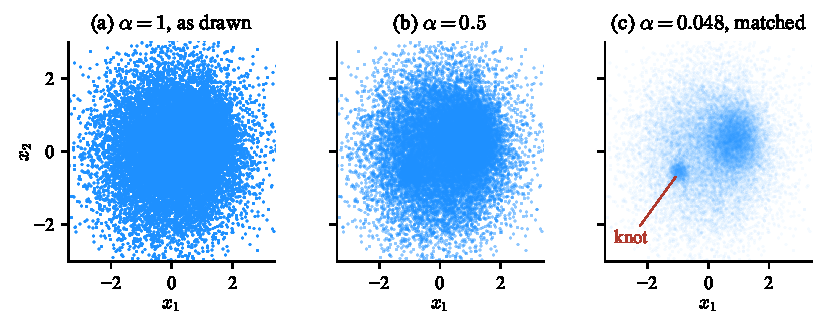
\includegraphics{plot_alpha}
	\caption{Twenty thousand points from a broad cloud holding a dense core and a small tight knot, drawn three ways on identical axes with identical $1.6$~pt markers. (a) At $\alpha = 1$, $88.0\%$ of the points land on ink that is already full, so the panel reports the outline of the cloud and the accident of draw order, and neither the core nor the knot survives. (b) At $\alpha = 0.5$, $54.0\%$ of them still do, because ink is $0.99$ of full by the seventh mark: halving the opacity does not halve the problem. (c) At $\alpha = 0.048$, which is $1/n_{\mathrm{typ}}$ for a measured typical overlap of $n_{\mathrm{typ}} = 21$ marks per marker footprint, the core and the knot both appear. The price is that a lone point now carries $4.8\%$ ink, near the edge of what can be seen at all.}
	\label{fig-plot-alpha}
\end{figure}

\emph{The same choice hides the isolated point.} An $\alpha$ small enough to resolve a crowd renders a lone mark at $\alpha$ of full ink and nothing more, $4.8\%$ in Fig.~\ref{fig-plot-alpha}(c), so the outlier that a scatter is often drawn to find is the first thing the setting removes. Where both matter, the two populations are two layers: the crowd at low $\alpha$, and the points that are alone drawn separately at full strength.

\begin{box_red}[Transparency is a magnitude channel without a key]
	A scatter at $\alpha < 1$ encodes count as darkness, so it falls under the rule of Sec.~\ref{sec-app-plot-matrix}: every magnitude channel needs a zero and a key. It has neither, and Eq.~\eqref{eq-plot-alpha-stack} is not linear in the count either, so the darkness cannot be read back even in principle. Use it to reveal that structure exists, never to report how much of it there is.
\end{box_red}

\begin{box_red}[PDF file size]
A transparent mark forces a transparency group into the PDFT. The twenty thousand markers of each panel of Fig.~\ref{fig-plot-alpha} make a $0.9$~MB file that is slow to open and slower to print. \textit{Rasterizing} the dense layer alone, keeps the axes and every label vector while the cloud becomes an image at the export resolution, and brings the same figure to $205$~kB. 
\end{box_red}


\FloatBarrier

\section{Ink That Carries No Data}\label{sec-app-plot-dataink}

Tufte's \emph{data-ink ratio} is the fraction of the ink on the page that encodes data. Everything else is either structure the reader needs, such as axis lines and tick labels, or decoration. Decoration is not neutral: it competes for the same attention the data needs, and the grouping laws of Sec.~\ref{sec-app-plot-gestalt} act on it just as readily.

\begin{figure}[ht]
	\centering
	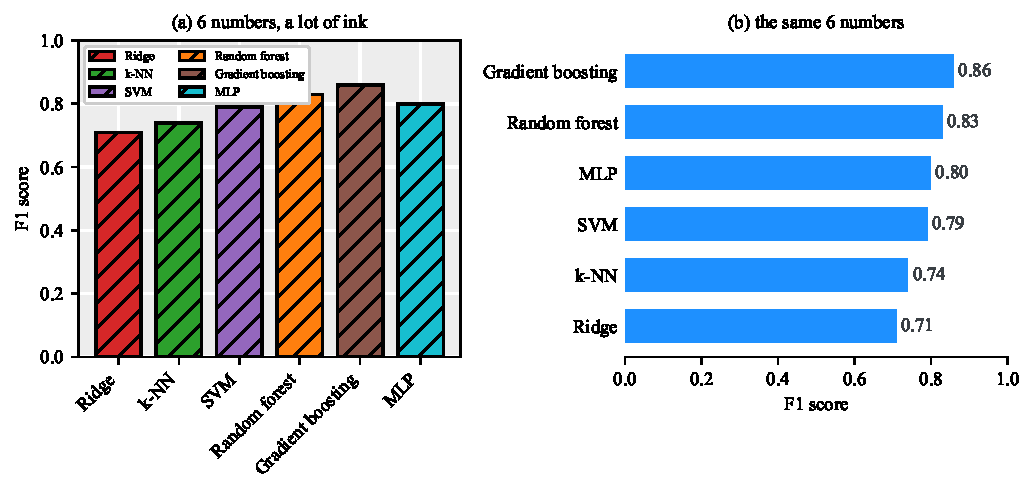
\includegraphics{plot_declutter}
	\caption{Six $F_1$ scores. (a) Defaults plus decoration: a gray panel, a full frame, a white grid over it, hatched fills, heavy outlines, tick labels rotated to fit, and a small-font legend that repeats the model names already on the axis and covers a bar while doing it. The model name is encoded three times over. (b) The same six numbers, sorted, horizontal so the names read normally, with the values printed at the bar ends so no axis lookup is needed.}
	\label{fig-plot-declutter}
\end{figure}

Panel~(b) removes nothing that a reader uses. 

\FloatBarrier


\section{Figures Inside a Document}\label{sec-app-plot-document}

A figure in a book or a paper is read on its own, out of order, before the surrounding text. Two requirements follow.

\paragraph{The figure must be self-contained}
Axes labeled with quantity and unit, series identified in the figure rather than in the body text, and any parameter the reader needs to interpret the panels stated in the caption. The test is whether a reader who has seen only this page can say what is plotted.

\paragraph{The caption states the finding, not the axes}
A caption reading ``Accuracy versus training set size'' repeats the axis labels and adds nothing. A caption reading ``Accuracy saturates beyond $2000$ samples, so the remaining error is not a data-quantity problem'' tells the reader what the figure is for. The captions throughout this document are written this way, and the numbers they quote are printed by the scripts that draw the figures, so the two cannot drift apart.

\paragraph{Export so the figure survives the page}
The conventions of this document are a worked instance of everything above: figures are drawn at the width they will occupy, so Eq.~\eqref{eq-plot-fontscale} gives $s = 1$ and the point sizes in the script are the point sizes on the page, and they are exported to PDF and SVG so they stay vector at any zoom, plus JPEG at $300$~dpi where a raster is needed. LaTeX then includes them without an extension, so the same source produces the PDF and the HTML build.


\section*{Further Reading}
%\subsubsection{Video}
\begin{itemize}
	\item \href{https://www.ted.com/talks/hans_rosling_the_best_stats_you_ve_ever_seen}{The best stats you've ever seen}, TED, Feb. 2006.
	\item \href{https://en.wikipedia.org/wiki/Anscombe%27s_quartet}{Wikipedia: Anscombe's quartet} and
	\href{https://doi.org/10.1080/00031305.1973.10478966}{Anscombe, ``Graphs in Statistical Analysis''} (\emph{The American Statistician}, 1973): four pages, and the origin of Fig.~\ref{fig-plot-anscombe}. The argument that a regression should never be reported without the scatter it was fitted to.
	\item \href{https://colorbrewer2.org}{ColorBrewer}, and \href{https://doi.org/10.1179/000870403235002042}{Harrower and Brewer, ``ColorBrewer.org''} (\emph{The Cartographic Journal}, 2003): the scheme families of Sec.~\ref{sec-app-plot-color}, with a picker that filters on colorblind-safe, print-safe and photocopy-safe.
	\item \href{https://www.nature.com/articles/nmeth.1618}{Wong, ``Points of View: Color Blindness''} (\emph{Nature Methods}, 2011): two pages, and the source of the eight-color palette used in Fig.~\ref{fig-plot-cvd}. See also \href{https://doi.org/10.1109/TVCG.2009.113}{Machado, Oliveira and Fernandes} (2009) for the simulation model behind that figure.
	\item \href{https://en.wikipedia.org/wiki/Color_blindness}{``Color blindness''} (Wikipedia): the conditions the second check of Sec.~\ref{sec-app-plot-checks} tests against --- which types exist, how common each is, and which pairs of colors they merge.
\end{itemize}


\subsubsection{Software}
\begin{itemize}
	\item \href{https://matplotlib.org/stable/plot_types/index.html}{\texttt{matplotlib}, plot types}: one thumbnail and one call per chart type, grouped by the kind of data. The fastest way to answer the ``which chart'' question of Sec.~\ref{sec-app-plot-encoding} without inventing something exotic.
	\item \href{https://matplotlib.org/stable/gallery/index.html}{\texttt{matplotlib}, the gallery}: the same catalog with complete runnable source for every figure, including the colormap comparisons of Sec.~\ref{sec-app-plot-color} and the small-multiple layouts of Sec.~\ref{sec-app-plot-many}.
	\item \href{https://www.mathworks.com/products/matlab/plot-gallery.html}{MATLAB plot gallery}: the MATLAB counterpart, organized the same way, for the figures produced by the scripts in \texttt{matlab/}.
	\item \href{https://www.mathworks.com/help/matlab/creating_plots/types-of-matlab-plots.html}{``Types of MATLAB Plots''}: the same catalog inside the documentation, indexed by data type, with the function name for each.
	\item \href{https://matplotlib.org/stable/users/explain/colors/colormaps.html}{``Choosing colormaps in Matplotlib''}: the sequential, diverging and qualitative families of Sec.~\ref{sec-app-plot-color}, with the gray level of each map plotted along it, which is the measurement behind Fig.~\ref{fig-plot-cmap-curve}.
	\item \href{https://colorbrewer2.org/}{ColorBrewer}: interactive scheme selection with color-blind-safe and print-safe filters, originally built for cartography and applicable unchanged to any categorical or sequential encoding.
	\item \href{https://colorcet.holoviz.org/}{\texttt{colorcet}}: colormaps beyond the \texttt{viridis} family that are built to the same rule --- equal steps in the data look like equal steps --- including maps designed for cyclic quantities such as phase.
	\item \href{https://matplotlib.org/stable/gallery/statistics/hexbin_demo.html}{\texttt{matplotlib}, \texttt{hexbin}}: the display to fall back on when a scatter is too dense for any opacity setting: the count per cell in one call, with the colorbar that $\alpha$ cannot carry and the log-count option that a heavy-tailed density needs.
	\item \href{https://datashader.org/}{\texttt{datashader}}: the same idea at the size where binning has to happen before the plot exists, tens of millions of points aggregated into the pixel grid of the figure rather than handed to the renderer as marks.
	\item \href{https://matplotlib.org/stable/gallery/specialty_plots/radar_chart.html}{\texttt{matplotlib}, radar chart}: the polygon of Sec.~\ref{sec-app-plot-radar} built on a polar axes, with the category-to-spoke transform written out, for the cases where the form is the right one.
	\item \href{https://matplotlib.org/stable/gallery/specialty_plots/hinton_demo.html}{\texttt{matplotlib}, Hinton diagram}: the square-area matrix of Fig.~\ref{fig-plot-matrix-forms}(a) in about twenty lines, including the sign handling that a signed weight matrix needs.
\end{itemize}

\subsubsection{Methods}
\begin{itemize}
	\item \href{https://doi.org/10.1080/01621459.1984.10478080}{Cleveland and McGill, ``Graphical Perception: Theory, Experimentation, and Application to the Development of Graphical Methods''} (\emph{J.\ American Statistical Association}, 1984): the experiments that produced the encoding ranking of Sec.~\ref{sec-app-plot-encoding}, and the source of the banking-to-$45^{\circ}$ rule.
	\item \href{https://doi.org/10.1145/1753326.1753357}{Heer and Bostock, ``Crowdsourcing Graphical Perception''} (CHI, 2010): the ranking replicated on a large sample, extended to rectangular area encodings and to chart sizes below the range Cleveland and McGill tested. Its third experiment is the chart-size and gridline-spacing study of Sec.~\ref{sec-app-plot-gridlines}, whose recommendation is that gridlines be separated by at least $8$ pixels and that chart height beyond $80$ pixels buys little on a $0$ to $100$ scale.
\item \href{https://doi.org/10.1111/cgf.12935}{Behrisch, Bach, Henry Riche, Schreck and Fekete, ``Matrix Reordering Methods for Table and Network Visualization} (\emph{Computer Graphics Forum}, vol.~35, no.~3, 2016): the sorting rule of Sec.~\ref{sec-app-plot-lookup} applied to the rows and columns of the matrix of Sec.~\ref{sec-app-plot-matrix}, with a survey of the algorithms and guidance on which to use for a given size and structure.
\item \href{https://doi.org/10.1101/gr.092759.109}{Krzywinski \emph{et al.}, ``Circos: An Information Aesthetic for Comparative Genomics} (\emph{Genome Research}, vol.~19, no.~9, 2009, pp.~1639--1645): the chord diagram on the data it is the right answer for, a genuine flow between many entities rather than the four near-equal levels of the matrix of Sec.~\ref{sec-app-plot-matrix}.
\item \href{https://doi.org/10.1145/964965.808606}{Porter and Duff, ``Compositing Digital Images} (\emph{SIGGRAPH}, vol.~18, no.~3, 1984, pp.~253--259): the paper that introduced the alpha channel and the \emph{over} operator of Eq.~\eqref{eq-plot-alpha-over}, whose repeated application is Eq.~\eqref{eq-plot-alpha-stack} and whose order dependence is Fig.~\ref{fig-plot-alpha-misuse}(a).
\item \href{https://doi.org/10.3138/J647-1776-745H-3667}{Flannery, ``The Relative Effectiveness of Some Common Graduated Point Symbols in the Presentation of Quantitative Data} (\emph{The Canadian Cartographer}, vol.~8, no.~2, 1971, pp.~96--109): why a circle whose area encodes a value is read slightly small, and the correction cartographers apply for it. The measurement behind the caution on Fig.~\ref{fig-plot-matrix-forms}(b).
\item \href{https://doi.org/10.1016/0004-3702(89)90049-0}{Hinton, ``Connectionist Learning Procedures} (\emph{Artificial Intelligence}, vol.~40, 1989, pp.~185--234): a survey from the period in which a weight matrix was routinely shown as a grid of scaled squares, the display that Fig.~\ref{fig-plot-matrix-forms}(a) is named after.
\item Tufte, \emph{The Visual Display of Quantitative Information} (2nd ed., 2001): data-ink ratio, chart junk and the lie factor, which are Sec.~\ref{sec-app-plot-dataink} and Sec.~\ref{sec-app-plot-axes} in their original form.
	\item Tufte, \emph{Visual Explanations} (1997), Ch.~2: the \emph{Challenger} analysis of Sec.~\ref{sec-app-plot-challenger}, reproducing the charts presented on the night and reconstructing what a temperature axis would have shown.
	\item \href{https://www.nasa.gov/history/rogersrep/genindex.htm}{\emph{Report of the Presidential Commission on the Space Shuttle Challenger Accident}} (1986): the primary source, including the O-ring damage record and the full set of charts of Fig.~\ref{fig-plot-thiokol}.
	\item \href{https://doi.org/10.1080/01621459.1989.10478858}{Dalal, Fowlkes and Hoadley, ``Risk Analysis of the Space Shuttle: Pre-Challenger Prediction of Failure''} (\emph{J.\ American Statistical Association}, 1989): the same data treated as a logistic regression, with the failure probability at $31\,^{\circ}$F and an honest account of how much the extrapolation can support.
	\item Few, \emph{Show Me the Numbers} (2nd ed., 2012): the pre-attentive feature list of Sec.~\ref{sec-app-plot-perception} and a practical treatment of tables, which most visualization books skip.
	\item \href{https://www.britannica.com/science/information-theory/Physiology}{\emph{Encyclop\ae dia Britannica}, ``Information theory: Physiology''}: the per-sense transmission rates of Table~\ref{tab-plot-senses} and the estimate of conscious throughput behind the compression argument of Sec.~\ref{sec-app-plot-perception}.
	\item Wong, \emph{The Wall Street Journal Guide to Information Graphics} (2010): one page per problem, in the before-and-after form of Fig.~\ref{fig-plot-declutter}.
	\item \href{https://doi.org/10.1109/VIS.2007.4629435}{Borland and Taylor, ``Rainbow Color Map (Still) Considered Harmful''} (\emph{IEEE Computer Graphics and Applications}, 2007): why \texttt{jet} produces the false boundaries of Fig.~\ref{fig-plot-colormap}, with examples from medical imaging where the artifacts were mistaken for findings.
	\item \href{https://doi.org/10.1038/s41467-020-19160-7}{Crameri, Shephard and Heron, ``The misuse of colour in science communication''} (\emph{Nature Communications}, 2020): a survey of colormap use across published work, with the perceptual-uniformity and color-blind-safety tests of Sec.~\ref{sec-app-plot-color} applied at scale.
	\item Munzner, \emph{Visualization Analysis and Design} (2014): the systematic treatment, organizing the whole field by what task the reader is performing and which channel serves it.
	\item \href{https://www.nvidia.com/en-us/training/teaching-kits/}{NVIDIA, Georgia Institute of Technology and Prairie View A\&M University, \emph{Accelerated Data Science Teaching Kit}}, Modules 7 and 8 (CC BY-NC 4.0): the course material this document was drafted from, covering the same ground as lecture slides with additional worked examples.
\end{itemize}


\appendix
\section{Tables}\label{sec-app-table}

A table is the right display when the reader looks values up by name (Sec.~\ref{sec-app-plot-lookup}), and it is subject to the same economy as a figure: every rule, color and digit either helps a reader find and compare numbers or competes with the numbers for attention. Unlike a figure, a table gets no help from the parallel stage of vision (Sec.~\ref{sec-app-plot-perception}). It is read serially, cell by cell, so its layout decides how long each look-up takes and whether a comparison can be made at all.

Each rule below is shown twice on the same numbers: (a) a counterexample that breaks it and (b) an example that follows it. Most of the tables use one running case, the six classifiers of Fig.~\ref{fig-plot-declutter}, with illustrative scores, fold-to-fold spreads and training times. Every one of those tables is sorted by its quantity of interest, best first, in both of its panels, so that the two panels differ only in the rule they illustrate: by F1 wherever F1 is shown, and by training time, fastest first, in the one table that shows only time. The exception is Sec.~\ref{sec-app-table-order}, where the row order is itself the rule under test.

\subsection{Table or figure}\label{sec-app-table-choice}

Use a table when the reader needs a few exact values, looked up by name, especially values with different units or values that will be copied elsewhere. Use a figure when the question is about shape: a trend, a minimum, a crossing, a group. The two directions fail differently, so both are shown.

\begin{figure}[ht]
	\centering
	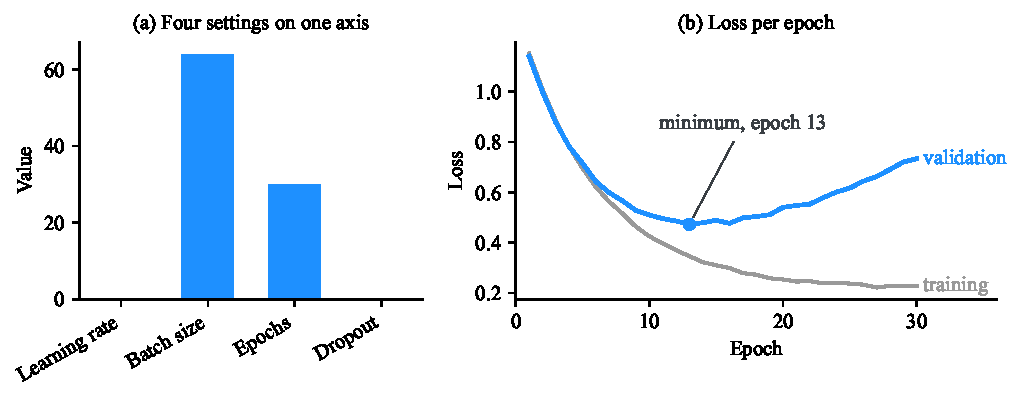
\includegraphics{plot_table_or_figure}
	\caption{(a) \textbf{Counterexample.} Four hyperparameters drawn as bars on one axis. They share no unit and span five orders of magnitude, so the learning rate and the dropout rate vanish, and the two visible bars cannot be read to the exact value that a reader copying the setup needs. (b) \textbf{Example.} Training and validation loss per epoch. The question is where validation stops improving, and the curve answers it at a glance: epoch 13, after which the gap to the training loss only grows.}
	\label{fig-table-choice}
\end{figure}

\begin{table}[ht]
	\centering
	\caption{The same two data sets in the other form. A handful of exact, mixed-unit settings reads best as a table; thirty losses do not.}
	\label{tab-table-choice}
	\begin{subtable}[t]{0.48\textwidth}
		\centering
		\caption{\textbf{Counterexample.} The losses of Fig.~\ref{fig-table-choice}(b), every second epoch. The minimum hides among fifteen similar rows, and the sampling a table forces has moved it: the smallest validation loss here is at epoch 16, not 13.}
		\small
		\begin{tabular}{rrr}
			\toprule
			Epoch & Training & Validation \\
			\midrule
			2 & 1.009 & 0.999 \\
			4 & 0.781 & 0.782 \\
			6 & 0.621 & 0.643 \\
			8 & 0.515 & 0.566 \\
			10 & 0.425 & 0.510 \\
			12 & 0.370 & 0.486 \\
			14 & 0.323 & 0.479 \\
			16 & 0.299 & 0.477 \\
			18 & 0.273 & 0.504 \\
			20 & 0.254 & 0.540 \\
			22 & 0.247 & 0.553 \\
			24 & 0.241 & 0.601 \\
			26 & 0.234 & 0.644 \\
			28 & 0.228 & 0.691 \\
			30 & 0.228 & 0.733 \\
			\bottomrule
		\end{tabular}
	\end{subtable}\hfill
	\begin{subtable}[t]{0.48\textwidth}
		\centering
		\caption{\textbf{Example.} The hyperparameters of Fig.~\ref{fig-table-choice}(a). Each value is exact, each carries its own unit, and each is found by name in one step.}
		\small
		\begin{tabular}{lr}
			\toprule
			Hyperparameter & Value \\
			\midrule
			Learning rate & $3\times10^{-4}$ \\
			Batch size & 64 \\
			Epochs & 30 \\
			Dropout rate & 0.1 \\
			\bottomrule
		\end{tabular}
	\end{subtable}
\end{table}

\begin{box_yellow}[One number is not a table]
	A single value, or two, belongs in the sentence. A table of one row makes the reader leave the text, find the float, and come back for nothing.
\end{box_yellow}

\FloatBarrier
\subsection{Round to what the data support}\label{sec-app-table-precision}

A digit is worth printing only if it could change a conclusion. When a score varies by $0.01$ from one cross-validation fold to the next, its third decimal is noise, and printing six decimals makes the reader parse four digits of noise per cell before reaching the two that matter. Ehrenberg's working rule is two \emph{effective} digits, the digits that vary across the column: they are what the eye can hold and compare. Round the spread to one or two significant digits and the value to the same decimal place.

\begin{table}[ht]
	\centering
	\caption{F1 score, mean $\pm$ standard deviation over five folds. Rounded to the spread, the ranking and its uncertainty read in one pass.}
	\label{tab-table-precision}
	\begin{subtable}[t]{0.48\textwidth}
		\centering
		\caption{\textbf{Counterexample.} Every digit the software printed.}
		\small
		\begin{tabular}{lr}
			\toprule
			Model & F1 \\
			\midrule
			Gradient boosting & $0.863127 \pm 0.012185$ \\
			Random forest & $0.829915 \pm 0.012074$ \\
			MLP & $0.801356 \pm 0.023712$ \\
			SVM & $0.790427 \pm 0.019866$ \\
			k-NN & $0.738562 \pm 0.028341$ \\
			Ridge & $0.713184 \pm 0.021507$ \\
			\bottomrule
		\end{tabular}
	\end{subtable}\hfill
	\begin{subtable}[t]{0.48\textwidth}
		\centering
		\caption{\textbf{Example.} The spread to one significant digit, the mean to the same decimal place.}
		\small
		\begin{tabular}{lr}
			\toprule
			Model & F1 \\
			\midrule
			Gradient boosting & $0.86 \pm 0.01$ \\
			Random forest & $0.83 \pm 0.01$ \\
			MLP & $0.80 \pm 0.02$ \\
			SVM & $0.79 \pm 0.02$ \\
			k-NN & $0.74 \pm 0.03$ \\
			Ridge & $0.71 \pm 0.02$ \\
			\bottomrule
		\end{tabular}
	\end{subtable}
\end{table}

\FloatBarrier
\subsection{Three horizontal rules, no vertical ones}\label{sec-app-table-rules}

A table needs three rules: one above the header, one below it, and one at the bottom. Columns are already separated by the white space between them, which the eye groups by proximity (Sec.~\ref{sec-app-plot-gestalt}); a vertical rule adds a line the reader has to cross on every comparison along a row. A full grid turns every cell into a box, and the boxes, not the numbers, become the dominant pattern on the page.

\begin{table}[ht]
	\centering
	\caption{The same twelve numbers in a grid and in the three-rule layout. The grid adds nine lines and no information.}
	\label{tab-table-rules}
	\begin{subtable}[t]{0.48\textwidth}
		\centering
		\caption{\textbf{Counterexample.} Vertical rules, a rule under every row, and a double rule under the header.}
		\small
		\begin{tabular}{|l|c|c|c|}
			\hline
			Model & F1 & Accuracy & Time (s) \\
			\hline\hline
			Gradient boosting & 0.86 & 0.89 & 41.2 \\
			\hline
			Random forest & 0.83 & 0.87 & 8.3 \\
			\hline
			SVM & 0.79 & 0.84 & 12.6 \\
			\hline
			Ridge & 0.71 & 0.78 & 0.4 \\
			\hline
		\end{tabular}
	\end{subtable}\hfill
	\begin{subtable}[t]{0.48\textwidth}
		\centering
		\caption{\textbf{Example.} Top, middle and bottom rules only; the columns are separated by space.}
		\small
		\begin{tabular}{lrrr}
			\toprule
			Model & F1 & Accuracy & Time (s) \\
			\midrule
			Gradient boosting & 0.86 & 0.89 & 41.2 \\
			Random forest & 0.83 & 0.87 & 8.3 \\
			SVM & 0.79 & 0.84 & 12.6 \\
			Ridge & 0.71 & 0.78 & 0.4 \\
			\bottomrule
		\end{tabular}
	\end{subtable}
\end{table}

\FloatBarrier
\subsection{Group with space and short rules}\label{sec-app-table-group}

When columns or rows fall into groups, show the grouping with the lightest device that works. A spanning header with a short rule under it (\verb|\cmidrule| in LaTeX) groups the columns beneath it, and a group label on its own row, set off by a little space, groups the rows. Full-width rules between groups and vertical rules between column blocks do the same job at a much higher ink cost, and they cut the table into boxes that the reader then has to reassemble.

\begin{table}[ht]
	\centering
	\caption{Validation and test scores for three families of models. The grouping is identical in the two versions; only the device that shows it differs.}
	\label{tab-table-group}
	\begin{subtable}[t]{\textwidth}
		\centering
		\caption{\textbf{Counterexample.} The column blocks are fenced by vertical rules, the families by full rules, and the family is repeated in a column of its own.}
		\small
		\begin{tabular}{|l|l||c|c||c|c|}
			\hline
			& & \multicolumn{2}{c||}{Validation} & \multicolumn{2}{c|}{Test} \\
			\hline
			Family & Model & F1 & Accuracy & F1 & Accuracy \\
			\hline
			Tree ensemble & Gradient boosting & 0.86 & 0.89 & 0.84 & 0.88 \\
			Tree ensemble & Random forest & 0.83 & 0.87 & 0.81 & 0.86 \\
			\hline
			Neural & MLP & 0.80 & 0.85 & 0.79 & 0.84 \\
			\hline
			Classical & SVM & 0.79 & 0.84 & 0.78 & 0.83 \\
			Classical & k-NN & 0.74 & 0.80 & 0.72 & 0.79 \\
			Classical & Ridge & 0.71 & 0.78 & 0.70 & 0.77 \\
			\hline
		\end{tabular}
	\end{subtable}

	\vspace{1em}
	\begin{subtable}[t]{\textwidth}
		\centering
		\caption{\textbf{Example.} Short rules under the spanning headers, and each family named once, on its own row.}
		\small
		\begin{tabular}{lrrrr}
			\toprule
			& \multicolumn{2}{c}{Validation} & \multicolumn{2}{c}{Test} \\
			\cmidrule(lr){2-3}\cmidrule(lr){4-5}
			Model & F1 & Accuracy & F1 & Accuracy \\
			\midrule
			\multicolumn{5}{l}{\textit{Tree ensembles}} \\
			\quad Gradient boosting & 0.86 & 0.89 & 0.84 & 0.88 \\
			\quad Random forest & 0.83 & 0.87 & 0.81 & 0.86 \\
			\addlinespace
			\multicolumn{5}{l}{\textit{Neural}} \\
			\quad MLP & 0.80 & 0.85 & 0.79 & 0.84 \\
			\addlinespace
			\multicolumn{5}{l}{\textit{Classical}} \\
			\quad SVM & 0.79 & 0.84 & 0.78 & 0.83 \\
			\quad k-NN & 0.74 & 0.80 & 0.72 & 0.79 \\
			\quad Ridge & 0.71 & 0.78 & 0.70 & 0.77 \\
			\bottomrule
		\end{tabular}
	\end{subtable}
\end{table}

\FloatBarrier
\subsection{Text left, numbers on the decimal point}\label{sec-app-table-align}

Text is read from its first letter, so text columns are left-aligned. Numbers are compared by magnitude, and magnitude is carried by the digits to the left of the decimal point, so numbers are aligned on it: with the same number of decimals in a column, the longer number is visibly the larger one, and the column works as a crude bar chart. Centered numbers lose that, because the position of the decimal point wanders from row to row. In LaTeX, the \texttt{S} column of the \texttt{siunitx} package aligns on the decimal point.

\begin{table}[ht]
	\centering
	\caption{Training time of the six models, fastest first. Aligned on the decimal point, each order of magnitude adds one digit of width, and the two slow models stand out by length alone.}
	\label{tab-table-align}
	\begin{subtable}[t]{0.48\textwidth}
		\centering
		\caption{\textbf{Counterexample.} Every column centered, with a varying number of decimals.}
		\small
		\begin{tabular}{cc}
			\toprule
			Model & Time (s) \\
			\midrule
			k-NN & 0.12 \\
			Ridge & 0.4 \\
			Random forest & 8.31 \\
			SVM & 12.6 \\
			Gradient boosting & 41.2 \\
			MLP & 95.7 \\
			\bottomrule
		\end{tabular}
	\end{subtable}\hfill
	\begin{subtable}[t]{0.48\textwidth}
		\centering
		\caption{\textbf{Example.} Names left-aligned, times aligned on the decimal point with one decimal throughout.}
		\small
		\begin{tabular}{lN{2.1}}
			\toprule
			Model & {Time (s)} \\
			\midrule
			k-NN & 0.1 \\
			Ridge & 0.4 \\
			Random forest & 8.3 \\
			SVM & 12.6 \\
			Gradient boosting & 41.2 \\
			MLP & 95.7 \\
			\bottomrule
		\end{tabular}
	\end{subtable}
\end{table}

\FloatBarrier
\subsection{Units in the header, one format per column}\label{sec-app-table-units}

A unit or a scale factor that applies to a whole column is stated once, in its header, and every cell of the column then uses the same unit, the same number format and the same number of decimals. Anything else makes the reader convert before comparing: $86\%$ against $0.85$, or \emph{1 min 36 s} against \emph{41 s}. A negative number takes a true minus sign ($-0.15$), not a hyphen (-0.15), which is shorter and sits at a different height.

\begin{table}[ht]
	\centering
	\caption{Accuracy, training time, and the F1 gap to the best model. Only the format differs between the two versions.}
	\label{tab-table-units}
	\begin{subtable}[t]{\textwidth}
		\centering
		\caption{\textbf{Counterexample.} Units in the cells, three formats for accuracy, four spellings of seconds, and hyphens for minus signs.}
		\small
		\begin{tabular}{lrrr}
			\toprule
			Model & Accuracy & Time & F1 gap \\
			\midrule
			Gradient boosting & 0.89 & 41 s & 0 \\
			Random forest & 87 \% & 8.3s & -0.03 \\
			MLP & 85\% & 1 min 36 s & -0.06 \\
			SVM & .84 & 12.6 sec & -0.07 \\
			k-NN & 80\% & 120 ms & -0.12 \\
			Ridge & 0.78 & 0.4 s & -0.15 \\
			\bottomrule
		\end{tabular}
	\end{subtable}

	\vspace{1em}
	\begin{subtable}[t]{\textwidth}
		\centering
		\caption{\textbf{Example.} Units in the headers, one format per column, true minus signs.}
		\small
		\begin{tabular}{lrrr}
			\toprule
			Model & Accuracy & Time (s) & F1 gap \\
			\midrule
			Gradient boosting & 0.89 & 41.2 & $0.00$ \\
			Random forest & 0.87 & 8.3 & $-0.03$ \\
			MLP & 0.85 & 95.7 & $-0.06$ \\
			SVM & 0.84 & 12.6 & $-0.07$ \\
			k-NN & 0.80 & 0.1 & $-0.12$ \\
			Ridge & 0.78 & 0.4 & $-0.15$ \\
			\bottomrule
		\end{tabular}
	\end{subtable}
\end{table}

\FloatBarrier
\subsection{Order the rows by what the reader wants}\label{sec-app-table-order}

Row order decides which question a table answers, exactly as it did for the chart of Fig.~\ref{fig-plot-lookup}. A results table is read for ranking, so its rows are sorted by the quantity of interest, and the best and worst models are then the first and last rows. Alphabetical order is the default of most software and serves only a reader who arrives with a name. When the rows have a natural order of their own (time, dose, model size), that order wins over both.

\begin{table}[ht]
	\centering
	\caption{Validation F1 of the six models. Sorted, the ranking is the table; alphabetical, it has to be reconstructed.}
	\label{tab-table-order}
	\begin{subtable}[t]{0.48\textwidth}
		\centering
		\caption{\textbf{Counterexample.} Alphabetical order: to find the runner-up the reader compares all six values.}
		\small
		\begin{tabular}{lr}
			\toprule
			Model & F1 \\
			\midrule
			Gradient boosting & 0.86 \\
			k-NN & 0.74 \\
			MLP & 0.80 \\
			Random forest & 0.83 \\
			Ridge & 0.71 \\
			SVM & 0.79 \\
			\bottomrule
		\end{tabular}
	\end{subtable}\hfill
	\begin{subtable}[t]{0.48\textwidth}
		\centering
		\caption{\textbf{Example.} Sorted by F1, best first: the ranking is read from top to bottom.}
		\small
		\begin{tabular}{lr}
			\toprule
			Model & F1 \\
			\midrule
			Gradient boosting & 0.86 \\
			Random forest & 0.83 \\
			MLP & 0.80 \\
			SVM & 0.79 \\
			k-NN & 0.74 \\
			Ridge & 0.71 \\
			\bottomrule
		\end{tabular}
	\end{subtable}
\end{table}

\FloatBarrier
\subsection{Compare down a column}\label{sec-app-table-transpose}

Numbers that are to be compared go in a column, one above the other. Down a column the digits of equal weight sit under each other, the decimal points line up, and the eye runs a short vertical path; along a row, each value is separated from the next by a whole cell and the digits no longer line up. The items being compared, here the models, are therefore the rows, and the measures are the columns. A table with more items than measures is also taller than it is wide, which is the shape a page holds.

\begin{table}[ht]
	\centering
	\caption{The six models on three measures. Transposed, each measure is one column of like numbers.}
	\label{tab-table-transpose}
	\begin{subtable}[t]{\textwidth}
		\centering
		\caption{\textbf{Counterexample.} Models as columns: every comparison between models runs along a row.}
		\small
		\begin{tabular}{lrrrrrr}
			\toprule
			& Gradient boosting & Random forest & MLP & SVM & k-NN & Ridge \\
			\midrule
			F1 & 0.86 & 0.83 & 0.80 & 0.79 & 0.74 & 0.71 \\
			Accuracy & 0.89 & 0.87 & 0.85 & 0.84 & 0.80 & 0.78 \\
			Time (s) & 41.2 & 8.3 & 95.7 & 12.6 & 0.1 & 0.4 \\
			\bottomrule
		\end{tabular}
	\end{subtable}

	\vspace{1em}
	\begin{subtable}[t]{\textwidth}
		\centering
		\caption{\textbf{Example.} Models as rows: each comparison runs down a column.}
		\small
		\begin{tabular}{lrrr}
			\toprule
			Model & F1 & Accuracy & Time (s) \\
			\midrule
			Gradient boosting & 0.86 & 0.89 & 41.2 \\
			Random forest & 0.83 & 0.87 & 8.3 \\
			MLP & 0.80 & 0.85 & 95.7 \\
			SVM & 0.79 & 0.84 & 12.6 \\
			k-NN & 0.74 & 0.80 & 0.1 \\
			Ridge & 0.71 & 0.78 & 0.4 \\
			\bottomrule
		\end{tabular}
	\end{subtable}
\end{table}

\FloatBarrier
\subsection{Emphasize sparingly}\label{sec-app-table-emphasis}

Emphasis in a table is the pre-attentive pop-out of Sec.~\ref{sec-app-plot-perception} put to work: one bold value in a column is found without a search. That works only while it is rare. Bold on every good value, a second color for another criterion and shading on alternate rows leave nothing standing out, and they add a conjunction search (which values are bold \emph{and} red?) that the reader cannot do at a glance. Mark the one thing per column the reader is looking for, usually the best value, and push the reference row back in gray rather than forward in color.

\begin{table}[ht]
	\centering
	\caption{The same results, emphasized two ways. With one mark per column, the winner of each measure is found without reading.}
	\label{tab-table-emphasis}
	\begin{subtable}[t]{0.48\textwidth}
		\centering
		\caption{\textbf{Counterexample.} Striped rows, every F1 and accuracy at or above $0.80$ in bold red, every time below $10$~s in blue.}
		\small
		\begin{tabular}{lrrr}
			\toprule
			Model & F1 & Accuracy & Time (s) \\
			\midrule
			\rowcolor{black!10} Gradient boosting & \textcolor{red}{\textbf{0.86}} & \textcolor{red}{\textbf{0.89}} & 41.2 \\
			Random forest & \textcolor{red}{\textbf{0.83}} & \textcolor{red}{\textbf{0.87}} & \textcolor{blue}{8.3} \\
			\rowcolor{black!10} MLP & \textcolor{red}{\textbf{0.80}} & \textcolor{red}{\textbf{0.85}} & 95.7 \\
			SVM & 0.79 & \textcolor{red}{\textbf{0.84}} & 12.6 \\
			\rowcolor{black!10} k-NN & 0.74 & \textcolor{red}{\textbf{0.80}} & \textcolor{blue}{0.1} \\
			Ridge & 0.71 & 0.78 & \textcolor{blue}{0.4} \\
			\bottomrule
		\end{tabular}
	\end{subtable}\hfill
	\begin{subtable}[t]{0.48\textwidth}
		\centering
		\caption{\textbf{Example.} The best value of each column in bold, the Ridge baseline in gray.}
		\small
		\begin{tabular}{lrrr}
			\toprule
			Model & F1 & Accuracy & Time (s) \\
			\midrule
			Gradient boosting & \textbf{0.86} & \textbf{0.89} & 41.2 \\
			Random forest & 0.83 & 0.87 & 8.3 \\
			MLP & 0.80 & 0.85 & 95.7 \\
			SVM & 0.79 & 0.84 & 12.6 \\
			k-NN & 0.74 & 0.80 & \textbf{0.1} \\
			\textcolor{gray}{Ridge (baseline)} & \textcolor{gray}{0.71} & \textcolor{gray}{0.78} & \textcolor{gray}{0.4} \\
			\bottomrule
		\end{tabular}
	\end{subtable}
\end{table}

\FloatBarrier
\subsection{Shade cells only for one homogeneous quantity}\label{sec-app-table-shade}

Shading each cell by its value turns a table into a heatmap: the pattern is seen at once, and the exact values stay readable. It is honest only when every shaded cell holds the same quantity on the same scale, as in the relations of Sec.~\ref{sec-app-plot-matrix}: a confusion matrix, a correlation matrix, a distance matrix. Shade a results table instead, and the reader applies one reading, darker is more, to columns with different units and different directions. Darker is better for F1 and worse for training time, and nothing in the color says so. The colormap choices of Sec.~\ref{sec-app-plot-colormap-scheme} apply unchanged: a sequential map for a quantity with a low and a high end, light enough at the top of the scale that the numbers stay legible.

\begin{table}[ht]
	\centering
	\caption{Shading is read as ``darker is more''. On a results table that reading makes the best model and the slowest one look alike; on a confusion matrix it shows the diagonal at once.}
	\label{tab-table-shade}
	\begin{subtable}[t]{0.48\textwidth}
		\centering
		\caption{\textbf{Counterexample.} One colormap over F1 and training time. The darkest cells are the best F1 and the slowest training, and they look alike.}
		\small
		\begin{tabular}{lrr}
			\toprule
			Model & F1 & Time (s) \\
			\midrule
			Gradient boosting & \cellcolor{blue!55}0.86 & \cellcolor{blue!26}41.2 \\
			Random forest & \cellcolor{blue!44}0.83 & \cellcolor{blue!9}8.3 \\
			MLP & \cellcolor{blue!35}0.80 & \cellcolor{blue!55}95.7 \\
			SVM & \cellcolor{blue!32}0.79 & \cellcolor{blue!11}12.6 \\
			k-NN & \cellcolor{blue!17}0.74 & \cellcolor{blue!5}0.1 \\
			Ridge & \cellcolor{blue!8}0.71 & \cellcolor{blue!5}0.4 \\
			\bottomrule
		\end{tabular}
	\end{subtable}\hfill
	\begin{subtable}[t]{0.48\textwidth}
		\centering
		\caption{\textbf{Example.} The confusion matrix of gradient boosting on three classes, as a percentage of each true class. One quantity, one scale, and the dark diagonal is the pattern.}
		\small
		\begin{tabular}{lrrr}
			\toprule
			& \multicolumn{3}{c}{Predicted (\%)} \\
			\cmidrule(lr){2-4}
			True class & Normal & Fault A & Fault B \\
			\midrule
			Normal & \cellcolor{blue!54}90 & \cellcolor{blue!4}6 & \cellcolor{blue!2}4 \\
			Fault A & \cellcolor{blue!9}15 & \cellcolor{blue!42}70 & \cellcolor{blue!9}15 \\
			Fault B & \cellcolor{blue!3}5 & \cellcolor{blue!6}10 & \cellcolor{blue!51}85 \\
			\bottomrule
		\end{tabular}
	\end{subtable}
\end{table}

\FloatBarrier
\subsection{A caption above the table that states the finding}\label{sec-app-table-caption}

A table caption goes above the table, because a table is read from the top and the reader should know what to look for before the first row. As with figures (Sec.~\ref{sec-app-plot-document}), the caption states what the table shows, not what it contains: the header row already says that the columns are F1 and accuracy.

\begin{table}[ht]
	\centering
	\caption{Placed above and stating the result, a caption tells the reader what to check before the first row is read. The pseudo-captions are set inside the panels, where each version puts them.}
	\label{tab-table-caption}
	\begin{subtable}[t]{0.48\textwidth}
		\centering
		\caption{\textbf{Counterexample.} A caption below the table that names its contents.}
		\small
		\begin{tabular}{lrr}
			\toprule
			Model & F1 & Accuracy \\
			\midrule
			Gradient boosting & 0.86 & 0.89 \\
			Random forest & 0.83 & 0.87 \\
			MLP & 0.80 & 0.85 \\
			\bottomrule
		\end{tabular}

		\medskip
		\textit{Table 3: Results.}
	\end{subtable}\hfill
	\begin{subtable}[t]{0.48\textwidth}
		\centering
		\caption{\textbf{Example.} A caption above the table that states the result.}
		\parbox{0.9\linewidth}{\raggedright\textit{Table 3: Gradient boosting leads on both measures, and its F1 margin over the random forest, $0.03$, is three times the fold-to-fold spread.}}

		\medskip
		\small
		\begin{tabular}{lrr}
			\toprule
			Model & F1 & Accuracy \\
			\midrule
			Gradient boosting & 0.86 & 0.89 \\
			Random forest & 0.83 & 0.87 \\
			MLP & 0.80 & 0.85 \\
			\bottomrule
		\end{tabular}
	\end{subtable}
\end{table}

\FloatBarrier
\subsection{Checklist}\label{sec-app-table-checklist}

Table~\ref{tab-table-checklist} collects the rules, in the order of this appendix, as the questions to ask of a table before it is published. It is built by them: three rules, text left-aligned, and the rows in their natural order, the order of the sections.

\begin{table}[ht]
	\centering
	\caption{Checklist for a table, one question per rule of this appendix.}
	\label{tab-table-checklist}
	\small
	\begin{tabular}{lll}
		\toprule
		Rule & Check & Sec. \\
		\midrule
		Table or figure & Read for exact values by name, not for a shape? & \ref{sec-app-table-choice} \\
		Precision & No digit finer than the uncertainty? & \ref{sec-app-table-precision} \\
		Rules & Three horizontal rules, no vertical ones? & \ref{sec-app-table-rules} \\
		Grouping & Groups shown by space, short rules, group rows? & \ref{sec-app-table-group} \\
		Alignment & Text left, numbers on the decimal point? & \ref{sec-app-table-align} \\
		Units & Units in the header, one format, true minus? & \ref{sec-app-table-units} \\
		Order & Rows sorted by what the reader wants? & \ref{sec-app-table-order} \\
		Direction & Compared values down a column? & \ref{sec-app-table-transpose} \\
		Emphasis & At most one mark per column? & \ref{sec-app-table-emphasis} \\
		Shading & Shaded cells all one quantity on one scale? & \ref{sec-app-table-shade} \\
		Caption & Above the table, stating the finding? & \ref{sec-app-table-caption} \\
		\bottomrule
	\end{tabular}
\end{table}

\FloatBarrier
\subsection*{Further reading}
\begin{itemize}
	\item \href{https://doi.org/10.2307/2344922}{Ehrenberg, ``Rudiments of Numeracy''} (\emph{J.\ Royal Statistical Society, Series A}, vol.~140, no.~3, 1977, pp.~277--297): the source of rounding to two effective digits, comparing down columns, ordering rows by size, and adding row and column averages as a focus.
	\item \href{https://doi.org/10.1017/bca.2020.11}{Schwabish, ``Ten Guidelines for Better Tables''} (\emph{J.\ Benefit-Cost Analysis}, vol.~11, no.~2, 2020, pp.~151--178): the rules of this appendix, and a few more, applied to six published tables redrawn before and after.
	\item \href{https://doi.org/10.1198/000313002317572790}{Gelman, Pasarica and Dodhia, ``Let's Practice What We Preach: Turning Tables into Graphs''} (\emph{The American Statistician}, vol.~56, no.~2, 2002, pp.~121--130): the other direction of Sec.~\ref{sec-app-table-choice}, tables from statistics journals that read better as figures.
	\item Few, \emph{Show Me the Numbers} (2nd ed., 2012): the chapters on table design, including when a table beats a graph.
	\item \href{https://ctan.org/pkg/booktabs}{Fear, the \texttt{booktabs} package manual}: the three-rule layout of Sec.~\ref{sec-app-table-rules} and the reasons for it, from the author of the package; and \href{https://ctan.org/pkg/siunitx}{the \texttt{siunitx} manual} for the \texttt{S} column of Sec.~\ref{sec-app-table-align}.
\end{itemize}


\end{document}
